% Memory complexity

% when memory is measured in machine words rather than bits
%https://stackoverflow.com/questions/34487306/is-this-function-for-loop-space-complexity-o1-or-on

%In computing, a word is the natural unit of data used by a particular processor design. A word is a fixed-sized piece of data handled as a unit by the instruction set or the hardware of the processor. %Modern processors, including embedded systems, usually have a word size of 8, 16, 24, 32, or 64 bits, while modern general purpose computers usually use 32 or 64 bits. Special
%https://en.wikipedia.org/wiki/Word_(computer_architecture)

%Auxiliary Space is the extra space or temporary space used by an algorithm.
%http://www.geeksforgeeks.org/g-fact-86/

%Analysis of algorithms typically focuses on the asymptotic performance, particularly at the elementary level, but in practical applications constant factors are important, and real-world data is in practice always limited in size. The limit is typically the size of addressable memory, so on 32-bit machines 232 = 4 GiB (greater if segmented memory is used) and on 64-bit machines 264 = 16 EiB. Thus given a limited size, an order of growth (time or space) can be replaced by a constant factor, and in this sense all practical algorithms are O(1) for a large enough constant, or for small enough data.
% https://en.wikipedia.org/wiki/Analysis_of_algorithms

% Array has a memory complexity of O(n) [ elements ]
% http://bigocheatsheet.com/

\section{Introduction}

In this chapter, we present our work on network centrality. Distributed systems are composed of independent connected nodes that coordinate their activities through communications in order to achieve common goals. Coordination in distributed systems often requires a single node to act as a leader and to perform some specific roles in the system. We address the issues of effectively and efficiently electing an approximate-centroid node or an approximate-center node in distributed embedded systems. 

The centroid is the set of nodes of minimum average distance to the others while the center is the set of nodes of minimum maximum distance to the others. These sets of nodes exhibit interesting properties for distributed system applications. For instance, centroid nodes are ideal nodes for hosting query-oriented service providers. Indeed, assuming that queries are likely to originate from any node in the network, placing service providers at the centroid minimizes the expected traveling distance for queries and answers, which implies low average time delays and message costs. To elect such nodes in an arbitrary asynchronous network, classical distributed algorithms require complete information about the network topology. Therefore, these algorithms are not scalable and not suitable for distributed embedded systems with limited computational, memory and energy resources.

Since modular robots form shapes, a first intuition is to use a geometric approach by computing the centroid of the configuration. In Figure~\ref{fig:centrality:shape-centers}, the {\em geometric centroid} is the point $C$ that stands in the middle of the object. Blocks in red represent the set of blocks that minimizes the worst-case network distance to all the other blocks. As we can see, the geometric centroid corresponds to a block in red for the grid shape and the S-line shape. However, for the torus, there is no block present at the location of the geometric centroid and all the blocks have the same worst-case distance. The case of the G-shape is even worse, as the geometric centroid of the shape leads to the worst case in terms of network distance. The S-line and G-line shapes are similar in the sense that they form a topological line and the block that minimizes the worst-case network distance stands in the middle of this line. There is an obvious mismatch between geometrical distances and network ones. Therefore, we need to consider network topologies instead of geometrical shapes and to use computations based on network distances instead of geometric ones.

Note that geometrical information could potentially still be used as a hint to start central node computation. Nevertheless, we decided to not use such information, in order to design generic distributed algorithms that do not rely on geometry.

\begin{figure}[!h]
	\centering
	\includegraphics[width=0.5\textwidth]{images/centrality/shapes.jpg}
	\caption{Difference between the geometric centroid (represented by C) and the Jordan center (in red). The Jordan center is defined as the set of nodes of minimum maximum distance to the others (see Section~\ref{section:centrality:centers}).\label{fig:centrality:shape-centers}}
\end{figure}

In this chapter, we consider a rather general system model. We assume a distributed system formed from an asynchronous non-anonymous point-to-point unweighted and undirected network in which nodes can only communicate with their immediate neighbors (neighbor-to-neighbor communication model). The complete system model is defined in Section~\ref{section:centrality:model}.

The contribution of this chapter is to propose a collection of both efficient and effective distributed algorithms to elect approximate-centroid and approximate-center nodes in asynchronous distributed systems. We propose the ABC-Center algorithm, the $k$-BFS SumSweep framework and the Probabilistic-Counter-based Central-Leader Election (PC2LE) framework. Frameworks are declined in two versions, one for approximate-center node election, another for approximate-centroid node election. Our algorithms and frameworks do not require any prior knowledge of the network, have a well-defined termination criterion, converge in a reasonable amount of time and are memory-efficient. The source code of our algorithms is available online\footnote{GitHub repository that hosts our algorithm codes for simulations: \VisibleSimUrl{}}\footnote{Official Blinky Blocks firmware repository in which some of our algorithm codes are hosted: \url{https://github.com/claytronics/oldbb}. At the time of submitting the final version of this manuscript, the $k$-BFS SumSweep and ABC-CenterV2 algorithms have been implemented for hardware Blinky Blocks.}.

In the $k$-BFS SumSweep, nodes compute their partial centrality value to a subset of root nodes composed of a random initial node and $k-1$ most external nodes. Root nodes are consecutively selected using the SumSweep approach that was originally proposed in the sequential algorithm for the exact radius and diameter computation of external graphs~\cite{borassi2014solvability}. Distributed \gls{bfses} are used for distributed \gls{sssp} computations. The main idea behind our framework is that central nodes are first and foremost central to the most external nodes. 

ABC-Center extends the sequential Minimax~\cite{handler1973minimax} and 4-Sweep~\cite{crescenzi2013computing} algorithms\footnote{Some examples of ABC-Center executions on Blinky Blocks systems are available online in video at \url{https://youtu.be/QxK12UAq42o} and \url{https://youtu.be/PYnJn6tXKa8}}. ABC-Center identifies an extreme path and recursively isolates midpoints on it until electing a single module. The main idea of ABC-Center is that central nodes lie in the middle of a diameter path. ABC-Center may be more convenient to use than the $k$-BFS framework as ABC-Center converges by itself, i.e., its termination does not rely on any input parameter.

\glsunset{bfs} % remove expansion
PC2LE is based on the input-graph analysis algorithms~\cite{kang2011centralities,kang2011hadi} and the distributed synchronous algorithm~\cite{garin2012distributed} which use low-memory-footprint probabilistic counters (e.g., Flajolet-Martin~\cite{flajolet1985probabilistic}, HyperLogLog~\cite{flajolet2007hyperloglog}) to estimate node centrality measures. In PC2LE, an estimated centrality value is computed for all nodes. PC2LE is approximately equivalent to running a \gls{bfs} from every node, but at less expense in terms of computations and communications. 

To test our algorithms and frameworks, we apply them to the Blinky Blocks (see Section~\ref{section:context:blinkyblocks}). Although we use modular robots to present and evaluate our algorithms, they work on all distributed systems that satisfy the assumptions detailed in Section~\ref{section:centrality:model}. We evaluate our algorithms both on hardware prototypes and through simulations. Experimental results show that our algorithms scale well accuracy, execution time, number of messages and memory usage. To the best of our knowledge, our algorithms are the most precise distributed algorithms to elect an approximate centroid or an approximate center in our target systems, with both a reasonable convergence time and a limited storage cost.

This chapter is organized as follows. In Section~\ref{section:centrality:model}, we define the system model. Afterwards, we provide a comprehensive overview of the existing centrality measures and definitions. Then, we discuss the related work in Section~\ref{section:centrality:related-work}. In Sections~\ref{section:centrality:k-bfs},~\ref{section:centrality:abc-center} and~\ref{section:centrality:pc2le} we respectively detail the $k$-BFS SumSweep framework, the ABC-Center algorithm, and the PC2LE framework. In Section~\ref{section:centrality:evaluation}, we provide experimental results. In Section~\ref{section:centrality:conclusion}, we conclude this chapter.

\section{System Model and Assumptions}
\label{section:centrality:model}

%Distributed system models
%https://www.labri.fr/perso/zemmari/dist/c1_models.pdf

\paragraph{System Model}
In this chapter, we consider distributed systems forming asynchronous non-anonymous point-to-point unweighted and undirected networks in which nodes can only communicate with their immediate neighbors (neighbor-to-neighbor communication model). Every node $v_i$ has a unique identifier, $id_{v_i}$. We assume that communication channels are FIFO (first in first out) and bidirectional , i.e., messages are received in the order in which they have been sent and the channels can carry messages in both directions (as in Section 1.1.1 of~\cite{raynal2013distributed}). Similarly to~\cite{awerbuch1985complexity}, we further consider that messages have a bounded length and may carry only a limited amount of information. Each message sent by a node to its neighbor arrives within some finite but unpredictable time.

Distributed algorithms often involve a resource-performance trade-off (e.g., memory usage, execution time, communication). We make design choices considering that our algorithms target large-scale \gls{lmr} ensembles.

\paragraph{Notation}
These systems can be modeled by an undirected and unweighted graph of inter-connected entities $G = (V, E)$, where $V$ is the set of vertices (representing the nodes), $E$ the set of edges (representing the connections), $|V|=n$, the number of vertices, $|E|= m$, the number of edges. $d(v_i,v_j)$ refers to the distance between vertices $v_i$ and $v_j$, i.e., the number of edges on a shortest path between $v_i$ and $v_j$. The diameter, $d$, of the network is defined as $d = \max\limits_{v_i \in V}\ \max\limits_{v_j \in V}\  d(v_i,v_j)$. $\Delta$ is the maximum network degree, i.e., the maximum number of neighbors that a node has in the network.

$N_{v_i}(h)$ represents the set of nodes within distance $h$ hops from node $v_i$ and $N_{v_i}^h$ represents the set of nodes exactly at distance $h$ hops from $v_i$. We assume that every node $v_i$ has a unique identifier $id_{v_i}$ and maintains a consistent list of its immediate neighbors $N_{v_i}^1$ using an external link-layer protocol. A message loss is considered to be a link failure and thus a neighbor departure.

\paragraph{Note on Complexity Calculation}

Unless otherwise mentioned, memory complexities are expressed in terms of machine words rather than in bits. Hence, we consider that a variable of a primitive data type (integer, boolean, etc.) uses $O(1)$ memory space. The number of values that can be encoded using variables may, however, induce limitations on the system size. For example, if node identifiers are encoded on $w$ bits, the system may contain at most $2^w$ nodes. 

The memory usage of a distributed algorithm is composed of both its application layer memory requirements and the space it needs to store messages. For instance, if during the execution of an algorithm that uses $O(1)$ space at the application layer, a module may simultaneously receive or send up to one message from/to all neighbors, this algorithm has a memory complexity of $O(\Delta)$.

Unless explicitly mentioned, we take into account message pileups in time and memory calculations.

%\subsection{The centrality does not hold}
\section{Network Centrality Metrics and Definitions}
\label{section:centrality:centers}

Graph and network centrality have been extensively studied in various domains such as in biology to identify the oldest metabolites~\cite{wuchty2003centers}, in social networks to find the most influential persons~\cite{hanneman2005introduction}, in computer networks to elect the most suitable root node to start message broadcasting~\cite{Korach:1984:DAF:579.585}, etc. Many metrics and definitions of centrality have been proposed. This section offers an overview of the most commonly used and their possible applications.

\subsection{Definitions}

The {\em Jordan center}~\cite{wasserman1994social} is the set of all nodes of minimum eccentricity, where the eccentricity $ecc(v_i)$ of a node $v_i$ is the maximum distance from $v_i$ to any other node (see Equations~\eqref{eq:eccentricity-1},\eqref{eq:eccentricity-2} and~\eqref{eq:center}). The inverse of the eccentricity is sometimes called the graph centrality~\cite{lehmann2003decentralized}. In this work, we use the term {\em center} to refer to the {\em Jordan center}. 

\begin{align}
\equationTextSize
\label{eq:eccentricity-1}
ecc(v_i) & = \max\limits_{v_j \in V} d(v_i,v_j)\\
\label{eq:eccentricity-2}
& = \min\argmax\limits_{r \in \mathbb{N}} |N_{v_i}(r)|
\end{align}

\begin{equation}
\equationTextSize
\label{eq:center}
Jordan\ Center = \{v_c \in V\ |\ ecc(v_c) = \min\limits_{v_i \in V} ecc(v_i) \}
\end{equation}

The {\em centroid}~\cite{dutot:hal-00742845} is the set of all nodes of minimum farness, where the farness $far(v_i)$ of a node $v_i$ is the sum of the distances to all the other nodes (see Equations~\eqref{eq:farness} and~\eqref{eq:centroid-sum}). The farness can be equivalently computed using the size of the sets of nodes at increasing hop distances~\cite{kang2011centralities} (see Equation~\eqref{eq:farness-2} and~\eqref{eq:farness-3}).

The centroid can be equivalently defined as the set of all nodes of maximum closeness, where the closeness $clo(v_i)$~\cite{freeman1979centrality} of a node $v_i$ is the inverse of its farness (see Equations~\eqref{eq:closeness} and~\eqref{eq:centroid-closeness}). The centroid can also be seen as the set of all nodes of minimum average distance to the others. The centroid is also called the {\em barycenter}~\cite{mamei2005self} or the {\em median}~\cite{Korach:1984:DAF:579.585} of the graph.

{
\equationTextSize
\begin{align}
\label{eq:farness}
far(v_i) & = \sum_{v_j \in V} d(v_i,v_j)\\
\label{eq:farness-2}
& = \sum_{r=1}^{d} r \times |N_{v_i}^r|\\
\label{eq:farness-3}
& = \sum_{r=1}^{d} r \times (|N_{v_i}(r)|\ - \ |N_{v_i}(r-1)|)
\end{align}
}

\begin{equation}
\equationTextSize
\label{eq:closeness}
clo(v_i) = \frac{1}{far(v_i)}
\end{equation}

{
\equationTextSize
\begin{align}
\label{eq:centroid-sum}
Centroid = & \{v_c \in V\ |\ far(v_c) = \min\limits_{v_i \in V}\ far(v_i)\}\\
\label{eq:centroid-closeness}
= &\{v_c \in V\ |\ clo(v_c) = \max\limits_{v_i \in V}\ clo(v_i)\}\\
\end{align}
}

The {\em center of gravity} or the {\em center of mass}~\cite{dutot:hal-00742845} is the set of all nodes of minimum weight, where the weight $we(v_i)$ of a node $v_i$ is the average of the squared distances to all the other nodes (see Equations~\eqref{eq:weight} and~\eqref{eq:center-of-mass}). In a graph with positive distances, the center of mass is equivalent to the centroid.

\begin{equation}
\equationTextSize
\label{eq:weight}
we(v_i) = \frac{1}{n} \sum_{v_j \in V} d(v_i,v_j)^2
\end{equation}

\begin{equation}
\equationTextSize
\label{eq:center-of-mass}
Center\ of\ mass = \{v_c \in V\ |\ we(v_c) = \min\limits_{v_i \in V}\ we(v_i)\}
\end{equation}

The degree centrality metric~\cite{freeman1979centrality} is based on the number of links a node possesses (see Equation~\eqref{eq:degree}). It is straightforward to compute it, but it only captures local information. This metric is not relevant in modular robots where modules have a bounded number of neighbors. Indeed, many of the modules will usually have the maximum number of neighbors a module can have. 

\begin{equation}
\equationTextSize
\label{eq:degree}
deg(v_i) = |\ \{ e\ |\ e = (v_i,v_j) \in E, v_j \in V \}\ |
\end{equation}

The betweenness centrality metric~\cite{freeman1979centrality} is based on how much a given node belongs to the shortest path of other nodes (see Equation~\eqref{eq:betweenness}). $\sigma_{v_jv_k}$ is the total number of shortest paths from node $v_j$ to node $v_k$ and $\sigma_{v_jv_k}(v_i)$ represents the number of those paths that pass through $v_i$. We choose to name the set of nodes of minimum betweenness the {\em betweenness center} (see Equation~\eqref{eq:betweenness-center}).

\begin{equation}
\equationTextSize
\label{eq:betweenness}
bet(v_i) = \sum_{\substack{v_j,v_k \in V\\v_i \neq v_j \neq v_k}} \frac{\sigma_{v_jv_k}(v_i)}{\sigma_{v_jv_k}}
\end{equation}

\begin{equation}
\equationTextSize
\label{eq:betweenness-center}
Betweenness\ center = \{v_c \in V\ |\ bet(v_c) = \max\limits_{v_i \in V}\ bet(v_i)\}
\end{equation}

For the sake of brevity, other centrality measures proposed in the literature (e.g., the stress centrality~\cite{shimbel1953structural} that reflects the volume of traffic that passes through a given node, the eigenvector centrality~\cite{bonacich1972factoring} which measures the influence of a node in a network, etc.) fall beyond the scope of this chapter. Recently, some low-complexity centrality measures that aim at approximate common centrality measures have been proposed (e.g., the tree-based centrality~\cite{kim2013leader}, the localized bridging centrality~\cite{nanda2008localized}, etc.). We choose to consider them as approximation algorithms and present those related to our work in the next section.

\subsection{Properties and Applications}
\label{section:centrality:centers:applications}

Figure~\ref{fig:centrality:centers} illustrates the differences between the different notions of center. The Jordan center is strongly influenced by the diameter of the system. The betweenness center is sensitive to critical paths between large sets of modules. Indeed, the modules that connect the two large squares are on all the paths between any module of the two squares.

\begin{figure}[!h]
	\centering
	\includegraphics[width=0.7\textwidth]{images/centrality/central-node-types.png}
	\caption{Differences between the different types of central module in a Blinky Blocks system.\label{fig:centrality:centers}}
\end{figure}


% Centrality and applications http://med.bioinf.mpi-inf.mpg.de/netanalyzer/help/2.7/index.html

In the context of distributed system applications, each type of central node has its own interesting properties. We assume that messages travel along the shortest paths. The Jordan center is suitable as initiator of parallel communications to all the other nodes, e.g., network flooding of broadcast messages. Flooding from the Jordan center minimizes the maximum traveling distance of the messages, which implies low maximum time costs. Centroid is ideal for unicast communications with all the other nodes, e.g., query-oriented services. Assuming that queries are likely to originate from any node, placing service providers at the centroid of the network minimizes the expected traveling distance for queries and answers, which implies low average time and message costs. The betweenness center is most useful for controlling and analyzing the network traffic. Indeed, the betweenness centrality of a node reflects the proportion of traffic that passes through this node. As a consequence, this measure favors nodes that join communities (i.e., dense subnetworks), rather than nodes that lie inside a community. The betweenness centrality can also be interpreted as a congestion sensitivity measure~\cite{lehmann2003decentralized}.

{
	\newcommand{\lenOneTwo}{0.225\linewidth}
	\newcommand{\lenTwoTwo}{0.32\linewidth}
	\newcommand{\lenTwoThree}{0.37\linewidth}
	\begin{center}
		\begin{table}[h!]
			\centering
			\small
			\begin{tabular}{|C{\lenOneTwo}|C{\lenTwoThree}|C{\lenTwoTwo}|}
				\hline				
				Time master position& Maximum pairwise difference (ms) & Mean absolute difference (ms)\\
				\hline
				% 3.5 hours; dense comm model, seed: 29535				
				extremity (front of the left arm) & 49.00 & 2.78 \\
				\hline
				center & 28.00 & 2.39 \\
				\hline
				centroid & 33.00 & 2.37 \\
				\hline
				betweenness center & 35.00 & 2.42 \\
				\hline
			\end{tabular}
			\caption{Impact of the position of the time master on the synchronization error in an enlarged version of the system depicted in Figure~\ref{fig:centrality:centers}. The system is synchronized using the Modular Robot Time Protocol (see Section~\ref{section:time-sync:protocol}). This system is composed of 1,456 nodes and has an 83-hop diameter. Every module in the system of Figure~\ref{fig:centrality:centers} is actually enlarged in a cube of 2x2x2 modules in this experiment. Results were computed on 3.5-hour-long simulations during which the synchronization error was measured every 3 seconds.}\label{table:centrality:time-master-position}
		\end{table}
	\end{center}
}

Table~\ref{table:centrality:time-master-position} shows the impact of the position of the time master on the synchronization error in an enlarged version of the Blinky Blocks system depicted in Figure~\ref{fig:centrality:centers}. The system is synchronized using the Modular Robot Time Protocol (see Section~\ref{section:time-sync:protocol}). As shown, placing the time master at a central node definitely leads to more synchronization precision. Moreover, placing the time master at the center (resp. centroid) tends to minimize the maximum (resp. average) synchronization error.

As shown in this section, existing types of central nodes have different features and applications. In this chapter, we propose efficient and effective algorithms to elect an approximate-center node or an approximate-centroid node.

\section{State of the Art}
\label{section:centrality:related-work}

As explained in the previous section, several types of centrality definitions exist. For conciseness reasons, we 
restrict our study to the work related to the center and to the centroid. For criticality centrality measures, the reader can refer to~\cite{nanda2008localized,tizghadam2010betweenness,kermarrec2011second,kang2011centralities}.

Existing algorithms for centrality computation can be categorized into four major families, namely exhaustive, graph-specific, sampling-based and probabilistic-counter-based. Other proposed approaches include tree-based computations, random-walk-based methods and linear programming approaches.

%https://cs.stackexchange.com/questions/51099/parallel-vs-distributed-algorithms/51160#51160
%https://en.wikipedia.org/wiki/Distributed_computing
Centrality computation is an active research topic in both the graph analysis and the distributed system communities. They address computation on graphs with two different perspectives, namely input-graph analysis and distributed computation on the network graph. In input-graph analysis algorithms, one or several computers perform calculations on (external) graphs provided as input. These algorithms can be sequential or, for higher performance, parallel and/or distributed. In distributed graph algorithms, the graph is the network itself and the nodes cooperatively self-perform computation on it, in a distributed fashion. These algorithms generally do not require nodes to hold a global view of the networks. This work is about distributed graph algorithms.

Only the algorithms for asynchronous distributed systems match our system model, but we still present the different approaches as they are closely related to our problem. We consider that 
recent advances in graph analysis should be taken into consideration to design efficient and scalable distributed algorithms.

%http://www.eecs.berkeley.edu/~jshun/kdd-final.pdf
%diffusion computation concept\cite{}

\subsection{Exhaustive Methods}

Exhaustive methods are exact and involve a distributed \gls{apsp} computation. We first discuss the \gls{apsp} problem and then present exhaustive approaches to compute node centrality.

Different methods exist to solve the \gls{apsp} problem in asynchronous networks. \gls{apsp} can be computed using the distributed Floyd–Warshall’s shortest path algorithm~\cite{toueg1980apsp} which runs in $O(n^2)$ time using $O(n^3)$ messages  with $O(n)$ messages that carry $O(n)$ distances~\cite{raynal2013distributed}. \gls{apsp} can also be computed using \gls{bfses}. Performing a single \gls{bfs} using Cheung's algorithm~\cite{cheung1983graph} takes $O(d)$ time, if we ignore message pileups, and uses $O(nm)$ messages~\cite{raynal2013distributed}. All nodes can initiate a \gls{bfs} traversal in parallel. However, the network may get congested, since messages will pileup, thus incurring a large time and memory overhead. On the other hand, \gls{bfses} can be performed one by one but it is expensive in terms of time. It uses in total $O(nd)$ time and $O(\Delta)$ space per node if message pileups are ignored. Also note that computing all the distances in parallel require the storage of $O(n)$ distances per node while, in sequential approaches, only the distance to the current-\gls{bfs} root along with the partial farness/eccentricity are stored per node and progressively updated.

An almost asymptotically optimal distributed synchronous \gls{apsp} algorithm has been proposed in~\cite{holzer2012optimal}. In this algorithm, a node triggers a \gls{bfs} traversal one time unit after having been visited by a depth-first search traversal. This ensures that \gls{bfses} do not collide. Thus, to compute its eccentricity/farness, a node only needs to store information about a single \gls{bfs} at a time. This algorithm runs in $O(n)$ synchronous rounds.

In~\cite{Korach:1984:DAF:579.585}, the authors propose algorithms to distributively elect the center and the centroid of graphs in different settings (asynchronous and synchronous networks, tree and arbitrary networks). The algorithms for asynchronous arbitrary networks use an exhaustive approach in which an initiator orders all nodes, through a depth-first search traversal of a spanning-tree, to compute their centrality value (eccentricity or farness), and then elects a node of minimum centrality value over the spanning tree. Any shortest path algorithm can be used to compute the distances from one node to all the others.

A distributed algorithm designed to elect the network centroid using $n$ parallel breadth-first network traversals without acknowledgment was proposed in~\cite{mamei2005self}. Each node initiates a \gls{bfs} by broadcasting a message that contains a hop counter increased at each hop. The authors claim that since the farness decreases monotonically to the centroid, nodes determine locally whether they are in the centroid or not by comparing their farness value to those of their neighbors. This algorithm converges but the termination is implicit, nodes do not have a defined global termination criterion. Some nodes may temporarily consider themselves as belonging to the centroid. Although this works in most situations, this local election mechanism is, for instance, not sufficient to elect a single centroid node in torus-like networks (see Figure~\ref{fig:centrality:shape-centers}-d)) where all nodes are centroid and they are not all neighbors to each other. This algorithm uses $O(n)$ memory space per node (we ignore message storage cost), as each node has to store a list of already known minimal distances to the other nodes to handle cycles.

In~\cite{lehmann2003decentralized}, Lehmann et al. propose a distributed synchronous framework to compute the eccentricity, closeness and betweenness of all nodes. Initially, all nodes broadcast a message that contains its unique node identifier and the currently traveled number of hops. Every node receives back a report message that contains an id-pair (source and destination) along with the distance between them. To avoid circles, every node constructs a data structure of $O(n^2)$ $id$-pairs.

A distributed synchronous algorithm dedicated to the computation of the eccentricity of all nodes along with the network radius and diameter was proposed~\cite{almeida2012fast}. It uses breadth-first search network traversals. Initially, all nodes initiate a \gls{bfs} traversal that contains its unique node identifier and a hop counter. Nodes progressively learned the distance to all the others. Local criteria to detect convergence in each node, using the computed values and the number of consecutive rounds with no new \gls{bfs} messages, are introduced. This algorithm requires the storage of $O(n)$ distances per node.

In~\cite{you2017distributed}, K. You et al. propose a distributed algorithm to compute the exact closeness centrality measures using only local interactions. At each round $r$, every node $v_i$ sends its set of $(r-1)$-hop neighbors to all its (1-hop) neighbors. Upon reception of these messages by all neighbors, a node $v_j$ can determine its set of $r$-hop neighbors using these messages and its own set of nodes within $r-1$ hops. This algorithm converges in $O(d)$ rounds but has a high storage cost per node as it ultimately requires the storage of $O(n)$ information. Moreover, the termination criterion relies on the knowledge of the diameter of the network, that can be distributively computed using the algorithm in~\cite{garin2012distributed}.

%implicit termination:  the algorithm has a finite execution and
%reaches a last configuration where each node of the system
%has the correct output.  However, the nodes do not know that
%they reached the last states of the execution of this algorithm.

As a consequence, existing asynchronous distributed algorithms designed to elect a node belonging to the exact center or centroid of arbitrary networks are not scalable. They involve a distributed \gls{apsp} computation which has either a large time complexity or/and a large storage cost in systems composed of thousands of nodes with constrained computational power and restricted memory resources.

\subsection{Methods for Specific Classes of Graphs}

Efficient heuristics have been proposed to compute the center and the centroid of tree graphs. 

For instance,~\cite{bruell1999self, patterson2014network} propose distributed methods to compute the center of a tree graph in $r$ rounds during which each node determines a sort of distance to the border of the network. The center is the set of nodes which have a greater value than all their neighbors. In~\cite{bruell1999self}, the authors also propose an algorithm to compute the centroid of a tree graph in $d$ rounds using a similar approach.

In~\cite{handler1973minimax}, the authors propose Minimax, an efficient sequential algorithm to compute the center of undirected tree graphs using only two \gls{bfses}. It picks A, a random node of the tree, B the farthest node from A and C the farthest node from B. The center is at midpoint of path between B and C. However, in arbitrary graphs, Minimax does not always return the exact center. For example, in Figure~\ref{fig:centrality:2sweep-4sweep}, Minimax returns one of the module in the diagonal in blue.

Other sequential algorithms for specific classes of graphs include~\cite{chepoi1994linear} for chordal graphs and~\cite{lan1999linear} for weighted cactus graphs. 

Although these approaches are efficient for the graphs they target, they are unfortunately not directly generalizable to arbitrary graphs.

\subsection{Sampling-based Methods}

Sampling-based methods consist in computing a sampling of values (shortest paths, node degree, etc.). These algorithms fall into two main categories, namely the approaches that compute shortest paths from a sampling of nodes and the methods that use limited-scope value computations.

\subsubsection{Shortest Paths from a Sampling of Nodes}

Some input-graph analysis approaches have recently been proposed in order to compute a central vertex of arbitrary graphs using a limited number of \gls{sssp} computations. Most of them use \gls{bfs} computations.

In~\cite{crescenzi2013computing}, Crescenzi et al. propose the 4-Sweep sequential algorithm which finds a node with low eccentricity in arbitrary graphs using 4 \gls{bfses}. It essentially performs two consecutive Minimax. $A^1$, $B^1$ and $C^1$ are selected exactly as in Minimax. Then, $A^2$ is selected as a node at midpoint between $B^1$ and $C^1$. Repeating Minimax a second time, $B^2$ is one of the farthest nodes from $A^2$ and $C^2$ is one of the farthest nodes from $B^2$. 4-Sweep returns a node at mid-distance between $B^2$ and $C^2$. In the general case, the 4-Sweep algorithm does not return the exact center. For instance, in Figure~\ref{fig:centrality:2sweep-4sweep}, 4-Sweep returns one of the nodes on the two diagonals, depending on the position of $A^1$ and $A^2$ just as Minimax would have done.

\begin{figure}[t!]
	\centering
	\includegraphics[width=0.75\textwidth]{images/centrality/twoSweepFourSweepFailure.png}
	\caption{Minimax and 4-Sweep failure case.\label{fig:centrality:2sweep-4sweep}}
\end{figure}

%\cite{shun2015evaluation} an evaluation of Parallel Eccentricity Estimation Algorithms on Undirected Real-World Graphs.

In~\cite{takes2013computing}, the authors propose a sequential algorithm to compute the exact eccentricity of all nodes using a limited number of consecutive \gls{bfses}. This algorithm refines lower and upper bounds on the vertex eccentricities until convergence is reached. 

In~\cite{borassi2014solvability}, Borassi et al. propose a similar sequential algorithm to find the exact radius (i.e., the eccentricity of the center) and diameter. The algorithm stops earlier as all the eccentricities are not computed. The authors suggest that the algorithm should start by performing some \gls{bfses} from the least central vertices and propose the SumSweep approach. In this approach, the root of the next \gls{bfs} is the node of minimum partial farness to the root of the previous \gls{bfses}, i.e., the nodes that maximize the sum to the roots of the previously performed \gls{bfses}. The complete algorithm may still require that a considerable number of \gls{bfses} should be performed, sometimes more than a hundred in Blinky Blocks systems composed of 500 modules\footnote{Based on practical experiments realized using our implementation of this algorithm, which is available online at: \GAURL{}}. A distributed implementation of the complete algorithm to find an exact center is, thus, not an option as performing a hundred distributed \gls{bfses} in a consecutive way will take too much time.

In~\cite{eppstein2001fast}, the authors propose a sequential algorithm to estimate node closeness using partial closeness computation from a random sample of nodes. In~\cite{dissler2016distributed}, the authors propose a distributed synchronous implementation of this algorithm. In this evaluation section, we show that performing \gls{bfses} from external nodes rather than from random ones leads to a better estimation of node centrality.

In~\cite{roditty2013fast,chechik2014better}, the authors propose input-graph analysis algorithms to estimate node eccentricity. These algorithms start to run some \gls{bfses} from a random sample of S nodes. Then they compute a \gls{bfs} from node $v$, one of the farthest node to any another node in S, and from a certain number of the closest nodes from $v$. Finally, they derive some estimation of the node eccentricities.

A sequential framework to approximate node closeness and node betweenness was introduced in~\cite{chan2009fast}. Closeness computations are performed on an abstract graph of small-diameter communities formed from tightly connected nodes.

All these existing approaches based on shortest paths computation from a sampling of nodes are promising but they do not fit our system model. They have been designed for input-graph analysis or target synchronous distributed systems.

\subsubsection{Limited-Scope Centrality Computation}

In Distributed Assessment of Network CEntrality (DANCE)~\cite{wehmuth2011distributed} and Distributed Assessment of the Closeness CEntrality Ranking (DACCER)~\cite{wehmuth2013daccer}, every node computes its volume centrality, i.e., the sum of the node degree of the $k$-hop neighboring nodes, using $O(k)$ time and $O(|N_{v_i}^k|)$ memory per node $v_i$. The value of $k$ impacts both the accuracy and the cost of these algorithms. $k$ should be large enough to derive an accurate global centrality value from localized computations. DANCE and DACCER are best suited to networks that do not present a highly regular structure, have a small diameter compared to their size and have a low density. As shown in Section~\ref{section:context:lmrs}, \gls{lmrs} do not exhibit these properties. In general, small-world (e.g., the Internet) or scale-free networks share such characteristics.

DANCE also builds a 3-level hierarchical structure that enables to locate both local and global central nodes. In large-scale systems, DANCE may have an important memory usage per node with regard to our strong storage restrictions for two reasons. Firstly, the number of neighbors at $k$ hops may be important, e.g., in the Blinky Blocks system, $|N_{v_i}(k)| = O(k^3)$ (see Sections~\ref{section:context:lmrs} and~\ref{section:appendixLMRs:diameter-blinkyblocks}). In terms of figures, the 2-hop neighborhood can be composed of up to 25 nodes, and the 3-hop neighborhood of up to 63 nodes. Secondly, the memory cost of the hierarchical structure can be important. Indeed, every node that exhibits a higher centrality value within a range of $(2k)$-hops, knows all the other nodes that satisfy the same property. This knowledge is then used to identify the highest centrality node in the whole network.

\subsection{Probabilistic-Counter-based Methods}

Algorithms based on low-memory-footprint probabilistic counters to estimate node centrality measures have recently been proposed in~\cite{kang2011hadi,kang2011centralities,garin2012distributed}. These algorithms are approximately equivalent to running a \gls{bfs} from every node but at less expense in terms of computations and communications.The algorithms run in $O(d)$ rounds. At each round $r$, nodes estimate the size of their $r$-hop neighborhood using local interactions with their 1-hop neighbors. The averaged farness can be estimated using equation~\eqref{eq:farness-3}. The eccentricity of a node is either estimated using equation~\eqref{eq:eccentricity-2} or corresponds to the last round at which the internal state of the probabilistic counter has been updated.

In~\cite{kang2011hadi,kang2011centralities}, the authors propose efficient input-graph analysis algorithms to respectively estimate the node averaged farness and eccentricity using the Flajolet-Martin probabilistic counter~\cite{flajolet1985probabilistic}. The algorithms terminate when no update has been performed for any node during a complete round. The internal state of a Flajolet-Martin counter is composed of $k$ bitstrings of $O(\log n)$ bits, with $k \geq 1$ an input parameter. These algorithms run in $O(dm)$ time and store $O(dk)$ bitstrings of $O(\log n)$ bits instead of an array of $O(n)$ information per node in naive sequential approaches. In practice, these algorithms even require storage for only two counter states per node, i.e., one for the previous and current rounds. These algorithms have been evaluated on a distributed implementation based on the MapReduce programming model for large-scale and distributed data processing. However, these implementations still require a global view of the graph.

A synchronous distributed algorithm built to estimate node eccentricity in anonymous networks has been proposed in~\cite{garin2012distributed}. It uses a statistical network size estimation algorithm~\cite{varagnolo2010distributed} which is based on random number generations and a max-consensus procedure. This algorithm converges in $O(d)$ time and needs to store $O(k)$ random numbers per node. In \cite{garin2012distributed}, the algorithm assumes the number of rounds to be provided as input or computed using an external algorithm.

Interesting probabilistic counter-based algorithms have been proposed but they do not fit our assumptions.

\subsection{Other Approaches}

\subsubsection{The Tree-based Centrality Measure}

In~\cite{kim2013leader}, the authors propose the tree-based centrality measure. It uses only distance calculations in $T(v_r)$, a \gls{bfst} of the network rooted at some random node $v_r$. The tree-based centrality of a node $v_i$ is equal to a fixed programmer-defined centrality weight $w_{c}$ with $w_{c} > 1$, if the height of $v_i$ in $T(v_r)$ is equal to the average distance to $v_r$. Otherwise, it is equal to 1. The authors suggest the combination of the tree-based centrality measure with other parameters, e.g., the remaining energy, to elect the more suitable node for a specific task. We name the set of nodes that maximize the tree-based centrality measure the tree-based center. Nodes with a height equal to the average distance to $v_r$ belongs to that center. As shown in~\cite{kim2013leader}, the closeness centrality and the expected tree-based centrality over all possible choices of $v_r$ and $T(v_r)$ have similar priorities. Therefore, we consider that the tree-based centrality is an approximation of the closeness centrality measure.

Electing a node in the tree-based center requires the election of an initiator and the construction of a single \gls{bfst} rooted at this initiator. This algorithm runs in $O(d)$ time and $O(\Delta)$ memory space per node.

\subsubsection{Random Walks}
An emergent approach to compute an approximate centroid of a distributed system is proposed in~\cite{dutot:hal-00742845}. A virtual ant colony explores the graph, virtually dropping pheromones on edges and nodes. The node that accumulates the largest amount of virtual pheromones is designated as the centroid. The main drawback of this method is that every ant must maintain a tabu list of visited nodes to handle cycles. This list is $O(n)$ memory space in the worst case. Moreover, the quality of the computed solution depends on the topology of the system. It performs well for trees but badly for grids.

%\cite{kermarrec2011second} Second order centrality: Distributed assessment of nodes criticity in complex networks SOC

\subsubsection{Linear Programming}

%In~\cite{wang2014distributed}, study  authors propose a distributed algorithm to compute the closeness on tree graphs using linear.
 
In~\cite{wang2015distributed}, the authors propose a scalable distributed algorithm to estimate node closeness centrality with only local interactions and a memory complexity per node of $O(\Delta)$. They define a regularized linear program based on the aggregation of a set of constraints that involves only nearby variables. A gradient algorithm is used to distributively solve this linear program over the network. The constraints of the linear program are augmented to its objective function as barriers and the algorithm converges progressively. An evaluation on networks with 6 to 50 nodes shows that this algorithm is on average 91\% accurate in terms of closeness ordering. However, this algorithm has no well-established termination criterion that would be desirable to use the closeness values to elect an approximate centroid of the system.

\subsection{Summary}

Table~\ref{table:centrality:related-work} summarizes the existing distributed algorithms. Computing exact center and centroid nodes in asynchronous distributed systems is an expensive operation in terms of messages and in terms of storage requirement and/or time. Algorithms designed for a specific class of graphs (e.g., tree graphs) are not generalizable to arbitrary graphs. Efficient sampling-based and probabilistic-counter-based methods have been proposed but they have not been applied to distributed asynchronous systems so far.

{
	\newcommand{\lenZero}{0.05\linewidth}
	\newcommand{\lenOne}{0.10\linewidth}
	\newcommand{\lenTwo}{0.11\linewidth}
	\newcommand{\lenThree}{0.16\linewidth}
	\newcommand{\lenFour}{0.22\linewidth}
	\newcommand{\lenFive}{0.35\linewidth}
	
	% Approaches: Exhaustive + 
	\newcommand{\MSG}{Method for specific classes of graphs}
	\newcommand{\SPSN}{Shortest path computations from a sampling of nodes}
	\newcommand{\LSCC}{Limited-scope centrality computation}
	\newcommand{\PCM}{Probabilistic-Counter-based method}
	\begin{table}[!t]
		
		\begin{center}
			\small
			\begin{tabular}
				{|C{\lenFour}|C{\lenFour}|C{\lenFive}|C{\lenOne}|}
				\hline
				Algorithm & Type of center or, if none, centrality measure & Approach & Async. vs Sync.\\
				\hline
				\cite{Korach:1984:DAF:579.585} & center, centroid & exhaustive & async  \\
				\hline
				\cite{lehmann2003decentralized} & closeness, eccentricity, betweenness & exhaustive & sync \\
				\hline
				\cite{almeida2012fast} & eccentricity & exhaustive & sync \\
				\hline
				\cite{you2017distributed} & closeness & exhaustive & UN \\
				\hline		
				BARYCENTER \cite{mamei2005self} & centroid & exhaustive & async \\
				\hline	
				\cite{bruell1999self} & centroid, center & \MSG{} (tree) & UN \\
				\hline
				\cite{patterson2014network} & center & \MSG{} (tree) & sync \\
				%\hline
				%\cite{wang2014distributed} & closeness & \MSG{} (tree) & sync \\
				\hline
				\cite{dissler2016distributed} & closeness & \SPSN{} & sync\\
				\hline
				DANCE~\cite{wehmuth2011distributed} DACCER~\cite{wehmuth2013daccer} & volume-based center$^*$ & \LSCC{} & async \\
				\hline
				\cite{garin2012distributed} & eccentricity & \PCM{} & async\\
				\hline
				\cite{dutot:hal-00742845} & centroid & Random walks & async \\
				\hline
				\cite{wang2015distributed} & closeness & Linear programming & async \\
				\hline
				\cite{kim2013leader} & tree-based center$^*$ & Computation on a tree & async\\		
				\hline
			\end{tabular}
		\end{center}
		
		{\small\hspace{3em} Our contributions:}
		\begin{center}
			\small
			\begin{tabular}
				{|C{\lenFour}|C{\lenFour}|C{\lenFive}|C{\lenOne}|}
				\hline
				$k$-BFS SumSweep & center, centroid & \SPSN{} & async \\
				\hline
				ABC-Center & center & \SPSN{} & async \\
				\hline	
				PC2LE & center, centroid & \PCM{} & async \\
				\hline
			\end{tabular}
		\end{center}
		\caption{Summary of the state of the art on network centrality in distributed systems. If the algorithm comes with an election mechanism, we provide the type of the elected (approximate) central node. Otherwise, we give the name of the computed/estimated centrality measure. Note $*$: a specific low-complexity measure is proposed and used to elect a most central node. ``UN'' stands for ``Unknown''.\label{table:centrality:related-work}}
	\end{table}
}

In this chapter, we propose asynchronous distributed algorithms to elect approximate-centroid and approximate-center nodes, namely ABC-Center, $k$-BFS SumSweep and Probabilistic-Counter-based Central-Leader Election (PC2LE). $k$-BFS SumSweep and ABC-Center are sample-based algorithms, i.e., they perform distributed \gls{bfses} from a sample of nodes, while PC2LE use probabilistic counting. 

$k$-BFS SumSweep is based on the sequential  SumSweep heuristic~\cite{borassi2014solvability}. ABC-Center extends the sequential Minimax~\cite{handler1973minimax} and 4-Sweep~\cite{crescenzi2013computing} algorithms. PC2LE is inspired by the input-graph analysis algorithms~\cite{kang2011centralities,kang2011hadi} and the distributed synchronous algorithm~\cite{garin2012distributed}. PC2LE differs from these approaches. First of all, PC2LE targets asynchronous distributed systems. Secondly, PC2LE uses its own mechanism to estimate the diameter of the system in order to bound the number of computation rounds. Thirdly, any probabilistic counter can be used in PC2LE and we have experimentally observed that, for similar resource usage, the HyperLogLog counter~\cite{flajolet2007hyperloglog} leads to more accuracy than the counters used in~\cite{kang2011centralities,kang2011hadi,garin2012distributed}. Finally, PC2LE comes with an election procedure to elect the most central node.

\section[Preliminary Materials on Network Traversal and Tree Algorithms]{Preliminary Materials on Network Traversal and Tree Algorithms%
	\sectionmark{Preliminary Materials on Network Traversal and Tree Algo...}}
\sectionmark{Preliminary Materials on Network Traversal and Tree Algo...}

\label{section:centrality:distributed-primitives}

This section presents the primitives used to design our algorithms.

\newcommand{\aspnesT}{ASPNES-BFS-ST-T}
\newcommand{\cheung}{CHEUNG-BFS-ST}
\newcommand{\cheungCb}{CHEUNG-BFS-ST-CB}
\newcommand{\cheungCbAgg}{CHEUNG-BFS-ST-CB-AGG}
\newcommand{\cheungIe}{LE\_CHEUNG-BFS-ST}
\newcommand{\cheungIeCb}{LE\_CHEUNG-BFS-ST-CB}
\newcommand{\cheungIeCbAgg}{LE\_CHEUNG-BFS-ST-CB\_STB-STC}

\subsection{Breadth-First Network Traversal and Spanning-Tree Construction}
\label{section:centrality:bfs}

Our centrality-based leader election algorithms are all based on \gls{bfst} constructions, which are used to compute distances and build paths to particular nodes. Constructing a \gls{bfst} enables one to solve the \gls{sssp} problem since the distance from a node to the root in the tree corresponds to the distance from that node to the root in the complete network.

\subsubsection{Algorithm Choice}

Building a spanning tree involves a time-communication trade-off~\cite{awerbuch1985distributed}. It requires at least $\Omega(d)$ time and $\Omega(m)$ messages~\cite{awerbuch1985distributed}. Different algorithms have been proposed for asynchronous systems.

Some of our algorithms (ABC-CenterV2 and $k$-BFS SumSweep) consecutively build a dozen or more \glspl{bfst}. It is crucial to use an algorithm that builds such a tree quickly in order to ensure an acceptable time of convergence for these algorithms. To the best of our knowledge, only Cheung's algorithm~\cite{cheung1983graph} and Aspnes' one~\cite{aspnesfall2017notes} run in $O(d)$ time (time due to message pileups is ignored here). Both of them use $O(\Delta)$ memory space at the application layer to store their neighbor states. Cheung's algorithm uses $O(nm)$ messages~\cite{lynch1996distributed} while Aspnes' algorithm uses $O(dm)$ messages.

\cheung{} refers to Cheung's algorithm. Aspnes' algorithm does not have a global termination (i.e., the root of the tree does not know when the tree construction is finished). Our algorithms require the detection of the global termination of the tree construction in order to continue their execution. In~\cite{boulinier2008space}, the authors show how to enhance Aspnes' algorithm with a global termination criterion. \aspnesT{} refers to the Aspnes' algorithm combined with that global termination detection method.

Figures~\ref{fig:centrality:bfs-time} and \ref{fig:centrality:bfs-messages} respectively show the simulated execution time and the number of messages used by the \cheung{} and the \aspnesT{} algorithms to construct a \gls{bfst} on random Blinky Blocks systems. The tree construction is initiated by the root node and the other nodes locally start to execute the algorithm upon reception of the first message. It appears Cheung's algorithm performs better, both in terms of time and messages than Aspnes' algorithm in our experimental setup. Thus, we decide to use  Cheung's algorithm with an optimization explained in the next section.

\begin{figure}[!h]
	\centering
	\includegraphics[width=\gnuplotGraphWidth]{images/centrality/ub/time}
	\caption{Simulated execution time of the \gls{bfst} construction and leader election algorithms.}
	\label{fig:centrality:bfs-time}
\end{figure}

\begin{figure}[!h]
	\centering
	\includegraphics[width=\gnuplotGraphWidth]{images/centrality/ub/messages}
	\caption{Total number of messages sent during the execution of the \gls{bfst} construction and leader election algorithms.}
	\label{fig:centrality:bfs-messages}
\end{figure}

\subsubsection{The Controlled-Broadcast Optimization}
\label{section:centrality-controlled-broadcast}

\cheung{} adopts an echo approach. Initially, the root of the tree under construction starts a network traversal by sending to all its immediate neighbors a BFS\_GO message which contains a hop counter initialized to 0. When a node receives a \mbox{BFS\_GO} message with a smaller hop counter than the previously known one, then it forgets about the previous network traversal and starts participating in the new one. BFS\_BACK messages are progressively sent back to the root node from the leaf nodes. The graph traversal terminates as soon as the root node gets notified by all its neighbors through BFS\_BACK messages.

As stated in~\cite{lynch1996distributed}, messages might pile up, which increases the execution time and the memory space usage. A module $v_i$ might, for instance, receive up to $|N_{v_i}^1|-1$ increasingly ``better'' BFS\_GO messages in such a short amount of time from all of its neighbors except $v_j$ and consequently insert $(|N_{v_i}^1|-1)$ BFS\_GO messages in the outgoing-message queue dedicated to $v_j$ in a so short amount of time that $v_i$ is not able to completely send a message to $v_j$. This outgoing-message queue keeps growing if this situation happens several times. Furthermore, if it happens many times, at many nodes, the system gets congested.

To avoid this situation, we propose the controlled-broadcast optimization. This optimization is inspired by~\cite{gallager1982distributed} where the author's suggestion is to send in priority BFS\_GO messages with a lower hop counter. In the controlled-broadcast optimization, a single BFS\_GO message is present in any outgoing-message queue at a time. If the firmware/operating system allows the modification of a queued message, we propose to update the currently queued BFS\_GO message (if there is any) rather than insert a new one in the queue. Otherwise, a node sends a new BFS\_GO message to a neighboring node only if the previous BFS\_GO message has been completely sent and removed from the outgoing-message queue. If the operating system enables to know when a message has been sent, this solution comes for free. Otherwise, nodes use an extra message to acknowledge every BFS\_GO message they receive and a node does not send a new BFS\_GO message until the previous one has been acknowledged. Note that this solution is not suitable in dense networks with shared communication medium where acknowledgment messages may cause many collisions.

We call Cheung's algorithm combined with the controlled-broadcast optimization the \cheungCb{} algorithm. The pseudo-code of \cheungCb{} is given in Algorithm~\ref{alg:centrality:bfs}.
%JB : Explique les notations utilisées dans l'algo : que le gris est à ajouter pour tel algo, le marron pour tel autre.


%\ulcorner;\urcorner;\llcornerand $\lrcorner$
%https://www.rpi.edu/dept/arc/training/latex/LaTeX_symbols.pdf

%\newcommand{\LEOnly}[1]{\textcolor{red}{#1}}
%\newcommand{\LEOnly}[1]{\underline{#1}}
%\newcommand{\LEOnly}[1]{[{#1}]}
%\newcommand{\LEOnly}[1]{($_\dag$#1$^\dag$}
%\newcommand{\LEOnly}[1]{$\llcorner$#1$\urcorner$~}
\newcommand{\LEOnly}[1]{\textcolor{gray}{$\llcorner$#1$\urcorner$}~}
%\newcommand{\LEOnly}[1]{~$_{+}$#1$_{+}$~}
%\newcommand{\LEOnly}[1]{[{#1}]}
%\newcommand{\LEOnly}[1]{~$_{\spadesuit}$#1$_{\spadesuit}$~}

% brown
\definecolor{myBrown}{RGB}{102,51,0}
\newcommand{\AggOnly}[1]{\textcolor{myBrown}{$_\dag$#1$^\dag$}}

\myAlgTwoPages{
	\Variants{
		{\nonl \cheungCb{}}\ \tcp{Black lines only}\\
		{\nonl {\LEOnly{\cheungIeCb{}}}}\ \tcp{Black + \LEOnly{\_\_\_} lines}\\
		\nonl {\AggOnly{\cheungCbAgg{}}}\ \tcp{Black + \AggOnly{\_\_\_} lines}\\
	}
	\BlankLine
	
	\Input{
		\nonl $N_{v_i}^1$ \tcp{\footnotesize $v_i$'s 1-hop neighborhood}\\
		{\nonl {$id_{v_i}$}\tcp{\footnotesize unique identifier of $v_i$}}\\
		\nonl {\AggOnly{$size$} \tcp{\footnotesize network size}}\\
		\nonl {\tcp{\footnotesize handler functions:}}
		\nonl {\AggOnly{$handleAppData$, $resetAppAggs$, $updateAppAggs$ and $getAppAggs$}}
	}
	\Output{
		\nonl {\tcp{\footnotesize Constructed tree (composed of $v_i$'s parent and $v_i$'s children):}}\\
		\nonl {$tree{<}parent,Children{>}$}\\
		\nonl {$distance$ \tcp{Distance of $v_i$ to the root of the tree}}\\
		\nonl {\AggOnly{$data$}\tcp{Ordered list of data propagated from the root}}
		\nonl {\AggOnly{$aggregates$}\tcp{Ordered list of aggregates computed on $v_i$'s subtree}}
	}
	
	\BlankLine
	\BlankLine
	{\bf Initialization} of node $v_i$:\\
	\label{alg:centrality:bfs:line:init1}
	$finished \gets false$;
	$tree.parent \gets \perp$;
	$tree.Children \gets \emptyset$;
	$Wait \gets \emptyset$\;
	\eIf(\tcp*[h]{(true for all nodes in \cheungIeCb{})}){$v_i$ root of the tree}{
		$distance \gets 0$;
		$id \gets id_{v_i}$;
	}{
		$distance \gets +\infty$; $id \gets \perp$;
	}
	\AggOnly{
		$data \gets \emptyset$;
		$branchSize \gets \emptyset$; 
		$resetAppAggs()$;
		$aggregates \gets {<}1{>} \cup getAppAggs()$;
	}\\

\BlankLine
\BlankLine
{\bf When} Algorithm variant {\bf starts} at node $v_i$ {\bf do}:\\
~\nonl\tcp{\footnotesize Executed by the root node only}
\ForEach{$v_j \in N_{v_i}^1$ } {
	{\bf send} BFS\_GO${<}id,distance,$\AggOnly{$data$}${>}$ {\bf to} $v_j$\;
	$Wait\gets Wait\cup \{v_j\}$\;
}
\If{$Wait= \emptyset$ } {
	Algorithm variant {\bf terminates}\label{alg:centrality:bfs:line:term2}\;
}
\label{alg:centrality:bfs:line:init2}

}{
\setcounter{AlgoLine}{13}
\BlankLine
\BlankLine

{\bf When} BFS\_GO($mid,dist$,\AggOnly{$dat$}$)$ {\bf is received by} $v_i$ {\bf from} $v_j$ {\bf do}:

\AggOnly{
	$data \gets dat$;
	$handleAppData()$;
}\\

\If{\LEOnly{$(mid < id)$} OR $id = \perp$}{
	$id \gets mid$; $distance \gets +\infty$; $tree.parent \gets \perp$;
}

\uIf{$(id = mid)$ AND $(dist+1 < distance)$} {
	\label{alg:centrality:bfs:line:new1}
	\If{$(tree.parent \neq \perp)$}{
		{\bf send} BFS\_BACK${<}id,distance-1,false,$\AggOnly{$\{\}$}${>}$ to $tree.parent$; \label{alg:centrality:bfs:line:back1}
	}
	
	$tree.parent \gets v_j$;
	$tree.Children \gets \emptyset$;
	$distance \gets dist+1$; 
	$Wait\gets \emptyset$\;			
	\AggOnly{
		$branchSize \gets \emptyset$\;
		$resetAppAggs()$;
	}\\
	\ForEach{$v_k \in N_{v_i}^1\ \backslash\ \{tree.parent\}$ } {
		{\bf send}  BFS\_GO${<}id$,$distance$,\AggOnly{$data$}${>}$ {\bf to} $v_k$.
		\tcc{\footnotesize Controlled-broadcast optimization (avoid congestion): send that message only if $v_i$'s outgoing queue to $v_k$ does not contain any other BFS\_GO message. Otherwise, wait until this message has been sent and then send the best known ${<}id,distance{>}$ value(s) at that future time in a BFS\_GO message}
		
		$Wait\gets Wait\cup \{v_k\}$\;
	}			
	\If{$Wait= \emptyset$}{
		$s \gets 1$; $aggregates \gets {<}s{>} \cup getAppAggs()$\;
		{\bf send} BFS\_BACK${<}id,distance-1,false,$\AggOnly{$aggregates$}${>}$ {\bf to} $tree.parent$;\label{alg:centrality:bfs:line:back2}
	}
	\label{alg:centrality:bfs:line:new2}
} 
\ElseIf{$id = mid$} {
	{\bf send} BFS\_BACK${<}mid$,$dist,false,$\{\}${>}$ {\bf to} $v_j$;  \label{alg:centrality:bfs:line:back3}
}

\BlankLine
\BlankLine

\BlankLine
\BlankLine

{\bf When} BFS\_BACK($mid,dist,c,$\AggOnly{$aggs$}) {\bf is received by} $v_i$ {\bf from } $v_j$ {\bf do}:

\If{$(id = mid)$ AND $(distance = dist)$ AND $\neg$ finished} {
	$Wait\gets Wait- \{v_j\}$\;
	\eIf{$c = true$} {
		$tree.Children \gets tree.Children \cup v_j$\;
		\AggOnly{
			$branchSize[v_j] \gets aggs[0]$}\label{alg:centrality:bfs:line:aggUpdate1}\;
	} {
	$tree.Children \gets tree.Children - v_j$\;
	\AggOnly{
		{\bf remove} $branchSize[v_j]$}\label{alg:centrality:bfs:line:aggUpdate2}\;
}

\AggOnly{
	\label{alg:centrality:bfs:line:aggUpdate3}
	$appAggUpdate(v_j,c,aggs)$;
}\\

\If{$Wait = \emptyset$} {
	\AggOnly{	
		$s \gets 1 + \sum_{v_k} branchSize[v_k]$;
	}\\
	\eIf{$tree.parent = \perp$} {
		$finished \gets true$\;
		\AggOnly{						
			\If{$s \neq size$} {
				\ShowLn \tcp{\footnotesize Wait (aggregate values may be uncorrect)}\label{alg:centrality:bfs:line:uncorrect}
				$finished \gets false$\;
				{\bf return}\;
			}
			$aggregates \gets {<}size{>} \cup getAppAggs()$;
		}\\
		Algorithm variant {\bf terminates}\label{alg:centrality:bfs:line:term2}\;
	}{
	\AggOnly{	
		$aggregates \gets {<}s{>} \cup getAppAggs()$;
	}\\
	{\bf send} BFS\_BACK${<}id, distance - 1, true,$\AggOnly{$aggregates$}${>}$ {\bf to} $tree.parent$\label{alg:centrality:bfs:line:back4}\;
}
}
}
%\end{multicols}
\caption{Pseudo-code for any code $v_i$ of different algorithms based on Cheung's \gls{bfst} algorithm: \cheungCb{}, \cheungIeCb{} and \cheungCbAgg{}.\label{alg:centrality:bfs}\vspace{1em}}
}

The controlled-broadcast optimization ensures that only $O(1)$ messages are present in any outgoing-message queue at a time. Thus, it prevents message pileups. It follows that there are at most $O(\Delta)$ messages at each node. Moreover, the algorithm variable memory usage is $O(\Delta)$. Hence, the total memory usage of \cheungCb{} is $O(\Delta)$. Moreover, the controlled-broadcast assumption does not change the asymptotic complexities (where pileups are ignored). The first two solutions come for free. In the third case, every BFS\_GO message is acknowledged, thus at most $O(2nm) = O(nm)$  messages are sent. Moreover, since there are at most $O(1)$ messages in every single outgoing-message queue, the best BFS\_GO message propagates through the network in $O(d)$ time. In this work, we use the third solution as it is the most general one, even though it is the most expensive one.

As shown in Figures~\ref{fig:centrality:bfs-queue}~and~\ref{fig:centrality:bfs-memory}, the controlled-broadcast optimization has no perceptible benefit on the maximum queue occupancy and the maximum memory usage of Cheung's algorithm in our experimental setup. This is because our optimization prevents a worst-case issue that rarely occurs in our target systems where the network is unloaded and all the links are configured with the same bitrate. However, our optimization has a significant impact on the maximum memory usage of the leader election algorithm based on Cheung's algorithm presented in the next section. Also note that the controlled-broadcast optimization only generates a low time and message overhead (see Figures~\ref{fig:centrality:bfs-time}~and~\ref{fig:centrality:bfs-messages}).

\begin{figure}[!h]
	\centering
	\includegraphics[width=\gnuplotGraphWidth]{images/centrality/ub/queue}
	\caption{Maximum queue length of the \gls{bfst} construction and leader election algorithms.}
	\label{fig:centrality:bfs-queue}
\end{figure}

\begin{figure}[!h]
	\centering
	\includegraphics[width=\gnuplotGraphWidth]{images/centrality/ub/memory}
	\caption{Maximum memory usage of the \gls{bfst} construction and leader election algorithms. Memory usage takes into account both the algorithm variables and the messages in the queues.}
	\label{fig:centrality:bfs-memory}
\end{figure}

%{
%	\newcommand{\lenOneL}{0.15\linewidth}
%	\newcommand{\lenTwoL}{0.09\linewidth}
%	\newcommand{\lenThreeL}{0.14\linewidth}
%	\newcommand{\lenFourL}{0.16\linewidth}
%	
%	\newcommand{\lenFiveL}{0.07\linewidth}
%	
%	\small
%	\begin{center}		
%		\begin{table}[h!]
%			\centering
%			\begin{tabular}{|C{\lenOneL}|C{\lenTwoL}|C{\lenFiveL}|C{\lenFiveL}|C{\lenThreeL}|C{\lenFourL}|}
%				\hline
%				Algorithm & Time & \multicolumn{2}{c|}{Messages} & Memory space & Local termination detection\\
%				\cline{3-4}
%				& & \# & Size & & \\
%				\hline
%				Update-based~\cite{cheung1983graph} & $O(d)$ & $O(nm)$ & $O(1)$ & $O(\Delta)$ & No\\
%				\hline
%				Layer-based~\cite{} & $O(d^2)$ & $O(m + dn)$ & $O(1)$ & $O(\Delta)$ & Yes\\
%				\hline
%				Aspnes~\cite{aspnesfall2017notes} & $O(d)$ & $O(dm)$ & $O(1)$ & $O(\Delta)$ & Yes\\
%				& $O(d log^3 n)$ & $O(m + n log^3 n)$ & $O(1)$ & ? & ?\\
%				
%			\end{tabular}
%			\caption{Existing algorithm to build a BFS spanning-tree in asynchronous systems.}\label{table:centrality:asynchronous-bfs}
%		\end{table}
%	\end{center}
%}
%Several approaches to construct breadth-first search spanning tree have been proposed in the literature
%Layered-BFS $O(d^2)$, $O(m + dn)$ messages.
%with centralized control: which is due to Y. Zhu
%and  Cheung (1987)—is based on a centralized control that allows each process to locally learn when its participation to the algorithm has terminated.

%p.554 Lynch Synchronizer.

%( ~\cite{boulinier2008space}).
%update messages and back messages. distance update messages.

\subsection{Leader Election based on Network Traversal Algorithms}
\label{section:centrality:id-leader-election}

Our centrality-based leader elections all start by electing an initiator.

Network traversal algorithms can be used to elect a leader~\cite{raynal2013distributed}. All nodes initiate concurrent parallel network traversals and a single one terminates. The node that initiates this traversal becomes the initiator. We call the leader election algorithm based on the \cheung{} algorithm the \cheungIe{}. At the end of \mbox{\cheungIe{}}, an initiator has been elected and a \gls{bfst} rooted at this node has been constructed. In addition, all nodes know their distance to the root.

\cheungIeCb{} refers to the \cheungIe{} combined with the controlled-broadcast optimization. Algorithm~\ref{alg:centrality:bfs} provides the pseudo-code of \cheungIeCb{}. In \cheungIeCb{}, nodes initiate $n$ concurrent \cheungCb{}. Thus, \cheungIeCb{} runs in $O(d)$ and uses $O(mn^2)$ messages and $O(\Delta)$ memory space per node.

We compare \cheungIe{} and \cheungIeCb{} to show the importance of the controlled-broadcast optimization in the leader election algorithm. As shown in Figure~\ref{fig:centrality:bfs-queue}, \cheungIeCb{} has a significantly lower maximum queue occupancy than \cheungIe{}. Hence, the controlled-broadcast optimization greatly reduces the maximum memory usage (see Figure ~\ref{fig:centrality:bfs-memory}), while it only generates a low time and message overhead (see Figures~\ref{fig:centrality:bfs-time}~and~\ref{fig:centrality:bfs-messages}).

\subsection{Broadcast and Convergecast on a Spanning Tree}
\label{section:centrality:stb-stc}

The Spanning-Tree Broadcast (STB) and Spanning-Tree Convergecast (STC) algorithms are two fundamental primitives used in distributed algorithms~\cite{lynch1996distributed,raynal2013distributed}.

In STB, some data are propagated down from the root of the spanning tree to all the nodes of the system along the edges of the tree. Algorithm~\ref{alg:centrality:stb} shows the pseudo-code of STB.

\newcommand{\STBSTCOnly}[1]{\textcolor{gray}{$\llcorner$#1$\urcorner$}~}

\myAlg{
	\Variants{
		{\nonl STB}\ \tcp{Black lines only}\\
		{\nonl {\STBSTCOnly{STB-STC}}}\ \tcp{Black + \STBSTCOnly{\_\_\_} lines}\\
	}
	
	\Input{
		\nonl $tree{<}parent,Children{>}$ \tcp{\footnotesize tree: $v_i$'s parent and Children}\\
		\nonl {$handleAppData$} \tcp{\footnotesize handler function}\\
		\nonl \STBSTCOnly{$updateAppAggs$} \tcp{\footnotesize handler function}
	}
	
	\Output{
		\nonl $data$\tcp{Ordered list of data propagated from the root}\\
		\nonl $aggregates$\tcp{Ordered list of aggregates computed over $v_i$'s subtree}
	}
	
	\Primitives{
		\nonl \STBSTCOnly{STC($tree: tree, handlers: updateAppAggs$)} \tcp{\footnotesize see Algorithm~\ref{alg:centrality:stc}}
	}
	
	\BlankLine
	\BlankLine
	{\bf Initialization} of node $v_i$:\\
	$data \gets \emptyset$;
	
	\BlankLine
	\BlankLine
	{\bf When} STB {\bf starts at} root node $v_i$ {\bf do}:\\
	\ForEach{$v_j \in tree.Children$} {
		{\bf send} STB\_GO($data$) {\bf to} $v_j$\;
	}
	
	\BlankLine
	\BlankLine
	{\bf When} STB\_GO${<}dat{>}$ {\bf is received by} $v_i$ {\bf from} $v_j$ {\bf do}:\\
	$data \gets dat$\;
	$handleAppData()$\;
	\STBSTCOnly{{\bf initialize} STC; {\bf start} STC;}\label{alg:centrality:line:stb-stc-start}\\
	\ForEach{$v_j \in tree.Children$} {
		{\bf send} STB\_GO${<}data{>}$ {\bf to} $v_j$\;
	}
	\caption{Pseudo-code for any code $v_i$ of the Spanning-Tree Broadcast (STB) algorithm with data propagation and the STB-STC (Spanning-Tree Broadcast followed by Spanning-Tree Convergecast) algorithm.\label{alg:centrality:stb}}
}

The STC algorithm is the inverse of STB. In STC, a convergecast message is forwarded back from the leaves to the root of the tree. Leaves start to send a convergecast message to their parent. Inner nodes wait until they have received a convergecast message from all their children before sending a convergecast message to their respective parent. The algorithm terminates once the root of the tree has received a convergecast message from all its neighbors. STC can be triggered by an STB (see Algorithm~\ref{alg:centrality:stb}, line~\ref{alg:centrality:line:stb-stc-start}). STB-STC refers to this combination of the execution of STB immediately followed by the execution of STC. Algorithm~\ref{alg:centrality:stc} shows the pseudo-code of STC. 

STB, STC and STB-STC use $O(d)$ time, $O(n)$ messages and require $O(\Delta)$ memory space per node, if we assume that the propagated and computed data can be stored using $O(1)$ memory space per node. These algorithms use only $O(1)$ variables, but they have a memory complexity of $O(\Delta)$ due to the storage cost of both the input spanning tree and the messages.

\myAlg{
		\Input{
			\nonl $tree{<}parent,Children{>}$ \tcp{\footnotesize tree: $v_i$'s parent and Children}\\
			\nonl {$updateAppAggs$} \tcp{\footnotesize handler function}\\
		}
		\Output{
			\nonl $aggregates$\tcp{Ordered list of aggregates computed over $v_i$'s subtree}\\
		}
		
		\BlankLine
		\BlankLine
		{\bf Initialization} of node $v_i$:\\
		\label{alg:centrality:stc:line:init1}
		$aggregates \gets {<}{>}$;
		$waiting \gets |tree.Children|$\;
		
		\BlankLine
		\BlankLine
		{\bf When} STC {\bf starts at} node $v_i$ {\bf do}:\\
		\If{$waiting = 0$}{
			\eIf{$tree.parent = \perp$}{
				STC {\bf terminates};
			}{
				{\bf send} STC\_BACK${<}aggregates{>}$ {\bf to} $tree.parent$\;
			}
		}
		
		\BlankLine
		\BlankLine
		{\bf When} STC\_BACK${<}aggs{>}$ {\bf is received by} node $v_i$ {\bf from} $v_j$ {\bf do}:\\
		$waiting \gets waiting - 1$\;
		$updateAppAggs(v_j,aggs)$\;	
		\If{$waiting = 0$}{
			\eIf{$tree.parent = \perp$}{
				STC {\bf terminates};
			}{
				{\bf send} STC\_BACK${<}aggregates{>}$ {\bf to} $tree.parent$\;
			}
		}
		\caption{Pseudo-code for any code $v_i$ of the Spanning-Tree Convergecast (STC) algorithm with aggregate computation.\label{alg:centrality:stc}}
}

\subsection{Global Data Diffusion and Global-Aggregate Computation}
\label{section:centrality:diffusion-aggregates}
%Pages: p.~56, and pp.~9-12
STB can be used to globally spread some information to all nodes in the system. STC can be used to compute network-wide aggregates~\cite{lynch1996distributed,raynal2013distributed} (e.g., the number of nodes in the system, the maximum distance to the root node, i.e., the height of the tree, the next hop on the path to a node that minimizes/maximizes a specific value, etc.). In this chapter, propagated data and aggregates are assumed to be stored using $O(1)$ memory space per node.

\cheungCb{} can also be used to spread information to all nodes in the network and to compute aggregates during the construction of a spanning-tree. \cheungCbAgg{} refers to the execution of \cheungCb{} during which some data is spread through the system and some aggregates are computed. The pseudo-code of \cheungCbAgg{} is provided in Algorithm~\ref{alg:centrality:bfs}. The information to be spread to all nodes is directly attached with the BFS\_GO messages. Computing aggregates about the tree (e.g., its height, path to the farthest node, etc.) during its construction is more tricky, as \cheungCb{} does not have a local termination criterion, i.e., a non-root node does not know when its involvement in the tree construction process is finished. Indeed, a node may finally leave a subtree for a better one at any time~\cite{raynal2013distributed}. Hence, a node maintains aggregate values of all its subtree branches and these partial aggregates are updated whenever a change occurs in its subtree (see Algorithm~\ref{alg:centrality:bfs}, lines~\ref{alg:centrality:bfs:line:aggUpdate1},~\ref{alg:centrality:bfs:line:aggUpdate2}~and~\ref{alg:centrality:bfs:line:aggUpdate3}). Moreover, it may happen that a leaf node finally leaves a subtree, whereas its previous parent has already initiated the BFS\_BACK wave, with a possibly wrong aggregate value, toward the root of the tree. The previous parent then initiates a second BFS\_BACK wave. This second wave, with the correct aggregated branch value, might possibly arrive anytime after the root has received a BFS\_BACK message from all its other branches (i.e., after having detected the termination of the tree construction and possibly after having launched some other processes which use the wrong computed value). To ensure that the last BFS\_BACK message has been received, we check that all nodes have participated in the aggregate computation only once. In order to do it, \cheungCb{} maintains at the root node a counter of the number of nodes that have participated in the aggregate computation. The value of this counter is compared to the actual network size which must be provided as input. The root node knows that the aggregate has been properly computed when these two values are equal (see Algorithm~\ref{alg:centrality:bfs}, line~\ref{alg:centrality:bfs:line:uncorrect}).

We do not assume that the network size is known at the system startup. In practice, our centrality-based leader election algorithms first elect an initiator using \cheungIeCb{} and then perform an STB-STC to compute the network size and other aggregates. \cheungIeCbAgg{} refers to this procedure. The pseudo-code of \cheungIeCbAgg{} is given in Algorithm~\ref{alg:centrality:bfs-ie-agg}. The value of the network size can then be used to control the execution of \cheungCb{}.

\myAlg{
		\Primitives{	
		\nonl \cheungIeCb\\
		\nonl STB-STC($tree: \text{\cheungIeCb}.tree, handlers: \perp, stcHandler$)\\
		}
		\BlankLine
		\BlankLine
		
		\nonl~\tcp{Initialization and start handlers:}
		{\bf Initialization} of $v_i$:\\
		$size \gets 1$;
		$height \gets 0$;
		$nextHopToFarthest \gets \perp$\;
		$\text{STB-STC}.aggregates \gets \{size,height\}$;
		
		\BlankLine
		\BlankLine
		{\bf When} \cheungIeCbAgg{} {\bf starts} at node $v_i$ {\bf do}:\\
		{\bf start} \cheungIeCb{}\;
		
		\BlankLine
		\BlankLine
		\nonl~\tcp{Primitive handlers for aggregate computation and data propagation:}
		\Fn{stcHandler($source,aggs$)}{
			$size \gets size + aggs[0]$\;
			\If{$height < aggs[1] + 1$}{
				$height \gets aggs[1] + 1$;
				$nextHopToFarthest \gets source$;
			}
			$\text{STB-STC}.aggregates \gets {<}size,height{>}$;
		}
		
		\BlankLine
		\BlankLine
		\nonl~\tcp{Primitive termination handlers:}
		{\bf When} \cheungIeCb{} {\bf terminates} at root node $v_i$ {\bf do}:\\
			{\bf start} STB-STC\;
			
		\BlankLine
		\BlankLine
		{\bf When} STB-STC {\bf terminates} at root node $v_i$ {\bf do}:\\
			\cheungIeCbAgg{} {\bf terminates}\;
			
		\caption{\cheungIeCbAgg{} detailed for any node $v_i$. \label{alg:centrality:bfs-ie-agg}}
}

\subsection{Robustness to Module Mobility and Faults}

To handle dynamic topology changes due to module mobility or to failure, a node launches a new central node election upon detection of a neighbor arrival or departure. Any local change may indeed have drastically changed the global topology of the network. Our algorithms are designed for fairly static networks where faults and node mobility only occur occasionally.

We use the technique proposed in~\cite{vasudevan2004design}. Each node participates in only one central node election at a time. In order to achieve this, an election index is used. This election index is a pair ${<}e,id{>}$ where $id$ is the identifier of the node that has initiated the election and $e$ is a number that is locally incremented each time a node triggers a new election. $id$ is used to break the tie among concurrent elections with the same $e$ value. A total order is defined on the election indices to determine election priority: ${<}e_1,id_1{>}$ has a higher priority than ${<}e_2,id_2{>}$ if $e_1 > e_2$ or if $e_1 = e_2$ and $id_1 < id_2$. Whenever a module receives a message for an election with a higher priority, it starts participating in this election and stops participating in any potential ongoing election of lower priority. 

Note that this mechanism is used as an underlying transparent service and does not appear in the description of our algorithms.

\newpage
\subsection{Summary of the Primitives and Notation}

Table~\ref{table:centrality:distributed-primitives} summarizes the properties of the different primitives used to build our centrality-based leader election algorithms.

{
	\newcommand{\lenZeroZero}{0.06\linewidth}
	\newcommand{\lenOneOne}{0.20\linewidth}
	\newcommand{\lenTwoTwo}{0.50\linewidth}
	\begin{center}
		\begin{table*}[!h]
			\small
			\centering
			\scalebox{1.0}{
				\begin{tabular}{|C{\lenOneOne}|C{\lenTwoTwo}|C{\lenZeroZero}|C{\lenZeroZero}|C{\lenZeroZero}|}
					\hline
					\multirow{3}{*}{Algorithm} & \multirow{3}{*}{Description} & \multicolumn{3}{c|}{Complexity}\\
					\cline{3-5}
					& & Memory space & Time & \# Messages\\
					\hline
					\cheungIeCbAgg{} & Elect the minimum-id node as a leader and construct a \gls{bfst} rooted at it. Then, perform a broadcast/convergecast to compute the size of the network along with  height of the tree and a path to the farthest node (see Section~\ref{section:centrality:diffusion-aggregates}). &  $O(\Delta)^*$ & $O(d)$ & $O(mn^2)$\\
					\hline
					\cheungCb{}($tree,handlers$) & Construct a \gls{bfst} rooted at the initiator with data propagation and aggregate computation using the handler functions (see sections~\ref{section:centrality:bfs}~and~\ref{section:centrality:diffusion-aggregates}). &  $O(\Delta)^*$ & $O(d)$ & $O(nm)$\\
					\hline
					STB($tree,handler$) & Broadcast on tree with data propagation. Data is handled using the input handler function (see sections~\ref{section:centrality:stb-stc}~and~\ref{section:centrality:diffusion-aggregates}). & $O(\Delta)^*$ & $O(d)$ & $O(n)$\\
					\hline
					STC($tree,handler$) & Convergecast on tree with aggregate computation using the input handler function (see sections~\ref{section:centrality:stb-stc}~and~\ref{section:centrality:diffusion-aggregates}). & $O(\Delta)^*$ & $O(d)$ & $O(n)$\\
					\hline
					STB-STC($tree,handlers$) & Broadcast, then convergecast on tree with data propagation and aggregate computation using the input handler functions (see sections~\ref{section:centrality:stb-stc}~and~\ref{section:centrality:diffusion-aggregates}). & $O(\Delta)^*$ & $O(d)$ & $O(n)$\\
					\hline
				\end{tabular}
			}
			\caption{Primitives used to build our centrality-based leader election algorithms. Note $^*$: in memory complexity calculation it is assumed that propagated and computed data can be stored using $O(1)$ memory space.}\label{table:centrality:distributed-primitives}
		\end{table*}
	\end{center}
}

\section{k-BFS SumSweep Framework}
\label{section:centrality:k-bfs}

The $k$-BFS SumSweep framework elects either an approximate center or an approximate centroid node of the system. We first describe the general idea of our framework. Then we provide a detailed description of its distributed implementation. Afterwards, we analyze the complexity of that implementation.

\subsection{Description at a Glance}

The $k$-BFS SumSweep framework is based on the SumSweep heuristic proposed as a starting point of the sequential algorithm in~\cite{borassi2014solvability} to compute the exact graph diameter and radius. SumSweep aims at consecutively selecting the most external vertices of a graph. Our distributed implementation of $k$-BFS SumSweep uses distributed \gls{bfses} to compute \gls{sssp}.

In our framework, a partial centrality value (eccentricity or farness, depending on the framework version) is computed for every node using distances to $\{u^\lambda\}_{1\leq \lambda \leq k} \subseteq V$, a subset of $k$ nodes, with $k \leq n$. This subset is formed from a random initial vertex and $k-1$ external vertices selected in a consecutive manner. The main idea behind our framework is that central nodes are first and foremost central to the most external nodes.

For pedagogical purposes, a sequential version of the $k$-BFS SumSweep framework is shown in Algorithm~\ref{alg:centrality:k-bfs-sequential}. Our framework runs in at most $k$ iterations. During each iteration $\lambda$, a node $u^\lambda$ is selected and the partial centrality value of every node is updated using the distance to $u^\lambda$ (line~\ref{alg:centrality:line:k-bfs-sequential:loop1}-\ref{alg:centrality:line:k-bfs-sequential:loop2}). $\{u^\lambda\}_{1<\lambda\leq k}$ are some of the most external nodes consecutively selected using the SumSweep heuristic, i.e., the next vertex is the vertex of maximum partial farness that has not been previously selected (line~\ref{alg:centrality:line:k-bfs-sequential:sumsweep}). Note than $u^1$ is selected at random as initially all partial farness values are null. In our distributed implementation, the node of minimum identifier is elected as $u^1$. At the end, the node of minimum partial eccentricity (resp. farness) is elected as the approximate center (resp. centroid) of the system (line~\ref{alg:centrality:line:k-bfs-sequential:end}).

\myAlg{		
	\Input{$G = (V,E)$ \tcp{\footnotesize network representation}\\
		\nonl $version \in \{center,centroid\}$\\
		\nonl $k$ \tcp {Number of nodes to select}
	}
	\Output{
		$centrality[\ ]$ \tcp{\footnotesize approximate eccentricity or farness of every node}\\
		\nonl $central$ \tcp{\footnotesize approximate center or centroid of the system}
	}
	
	\ForEach{$v_i \in V$} {	
		$far[v_i] \gets 0$\;		
		$centrality[v_i] \gets 0$\;
	}
	$Candidates \gets V$\;
	
	\For{$\lambda = 1$ to $min\{k,n\}$} {
		\label{alg:centrality:line:k-bfs-sequential:loop1}
		$u \gets v_i \in \argmax\limits_{v_j \in Candidates}
		far[v_j]$\label{alg:centrality:line:k-bfs-sequential:sumsweep};\ \tcp{SumSweep heuristic (ties are broken arbitrarily)}
		
		$Candidates \gets V - \{u\}$\;
		
		\ForEach{$v_i \in V$} {
			$far[v_i] \gets far[v_i] + d(u,v_i)$\label{alg:centrality:line:k-bfs-sequential:computation1}\;
			\eIf{$version = center$}{
				$centrality[v_i] \gets \max \{centrality[v_i], d(u,v_i)\}$\;
			}{					
				$centrality[v_i] \gets far[v_i]$\;
				\label{alg:centrality:line:k-bfs-sequential:computation2}
			}
		}
		\label{alg:centrality:line:k-bfs-sequential:loop2}
	}
	$central \gets v_i \in \argmin\limits_{v_j\in V} centrality[v_j]$;\label{alg:centrality:line:k-bfs-sequential:end}\ \tcp{a node of minimum centrality value is elected}
	\caption{Sequential version of $k$-BFS SumSweep framework.\label{alg:centrality:k-bfs-sequential}}
}

Figure~\ref{fig:centrality:k-bfs} depicts an execution of the $k$-BFS SumSweep framework on a 200-node Blinky Blocks system with $k = 10$. For both the center and centroid versions, the elected node is close to the theoretical node. In the evaluation section, we show that $k = 10$ provides accurate results even with large-scale systems of $10^4$ nodes.

\begin{figure}[!h]
	\centering
	\includegraphics[width=0.75\linewidth]{images/centrality/k-bfs-sumsweep}
	\caption{The k-BFS SumSweep framework running on a random two-dimensional Blinky Blocks system composed of 200 modules with $k= 10$. The initial module from which is performed the first distance computation is in brown. The other $k-1$ external nodes selected are in yellow and the order of selection is written on them. In the center version of our framework, the  module in red is elected and it matches the theoretical center. In the centroid version, the module in cyan is elected while the exact centroid is the (nearby) module in grey.\label{fig:centrality:k-bfs}}
\end{figure}

\subsection{Distributed Implementation}

Algorithm~\ref{alg:centrality:k-bfs-distributed} provides the pseudo-code of our distributed implementation of the $k$-BFS SumSweep framework. It uses two of our primitives (\cheungIeCbAgg{} and \cheungCbAgg{}) and two specific types of messages (NEXT\_BFS and ELECTED).


\myAlgTwoColsTwoPagesLarger{
	\Input{
		$version \in \{center,centroid\}$\\
		\nonl $k$ \tcp {Number of BFSes to perform}
	}
	
	\Output{
		a single central node is elected	
	}
	
	\Primitives{	
		\nonl \cheungIeCbAgg{}\\
		\nonl \cheungCbAgg{}($handlers: handleBFSData, updateBFSAggs, getBFSAggs,$\\
		\nonl ~~~$resetBFSAggs$)\\
	}
	\BlankLine
	\BlankLine	
}{
	\nonl~\tcp{Initialization and start handlers:}
	{\bf Initialization} of $v_i$:\\
	$candidate \gets true$; $iteration \gets 0$; $far \gets 0$
	$centrality \gets 0$; $branchCentrality \gets \{\}$; $branchFarCandidate \gets \{\}$;	
	$nextHopToMinCentrality \gets \perp$; $nextHopToMaxFarCandidate \gets \perp$\;
	{\bf start} $k$-BFS SumSweep\;
	
	\BlankLine
	\BlankLine
	{\bf When}  $k$-BFS SumSweep {\bf starts} at node $v_i$ {\bf do}:\\
	{\bf start} \cheungIeCbAgg{}\label{alg:centrality:line:k-bfs-distributed-initiator-start}\;
	%\Indm
	
	\BlankLine
	\BlankLine
	\nonl~\tcp{Helper functions:}
	\Fn{updateLocalValues()
		\label{alg:centrality:line:k-bfs-distributed-update-1}}{
		$dist \gets \text{\cheungCbAgg{}}.distance$\;
		\If{$iteration = 1$}{
			$dist \gets \text{\cheungIeCbAgg{}}.distance$\;
		}
		$far \gets far + dist$\;
		\eIf{$version = center$}{
			$centrality \gets \max \{centrality, dist\}$\;
		}{					
			$centrality \gets far$\;
		}
	}\label{alg:centrality:line:k-bfs-distributed-update-2}
	
	\nonl~\tcp{Primitive handlers for aggregate computation and data propagation:}
	\Fn{handleBFSData()}{
		$iter \gets \text{\cheungCbAgg}.data[0]$\;
		\If{$iter > iteration$}{
			$iteration \gets iter$\;
			updateLocalValues()
			\label{alg:centrality:line:k-bfs-distributed-update-4}\;
			\nonl~\tcp{Take part in this BFS as non-root:}
			{\bf re-initialize} \cheungCbAgg{}\;
		}
	}
	\Fn{resetBFSAggs()}{
	$branchCentrality \gets \{\}$; $branchFarCandidate \gets \{\}$\;
	}\label{alg:centrality:line:k-bfs-distributed-bfs-aggs-2}
	\Fn{updateBFSAggs($v_j, child, aggs$)
		\label{alg:centrality:line:k-bfs-distributed-bfs-aggs-1}}{
		\eIf{$child = true$}{
			$branchCentrality[v_j] = aggs[1]$\;
			$branchFarCandidate[v_j] = aggs[2]$\;
		}{
			{\bf remove} $branchFarCandidate[v_j]$\; 
			{\bf remove} $branchCentrality[v_j]$\;
		}
	}		
	\Fn{getBFSAggs()\label{alg:centrality:line:k-bfs-distributed-bfs-get-aggs-1}}{
		$dist \gets \text{\cheungCbAgg{}}.distance$\;
		\nonl~\tcp{Maximum candidate farness:}
		$maxCandidateFar \gets 0$; $nextHopToMaxFarCandidate \gets \perp$\;
		\If{$candidate = true$}{
			$maxFar \gets far + dist$\;
		}
		$v_f \gets \argmax_{v_k \in N_{v_i}^1} branchFarCandidate[v_k]$\;
		\If{$v_f \neq \perp$ AND $branchFarCandidate[v_f] > maxFar$}{
			$maxCandidateFar \gets branchFarCandidate[v_f]$;
			$nextHopToMaxFarCandidate \gets v_f$\;					
		}
		\nonl~\tcp{Minimum centrality value:}
		\eIf{$version = center$}{
			$minCentrality \gets \max \{centrality, dist\}$\;
		}{					
			$minCentrality \gets centrality + dist$\;
		}
		$nextHopToMinCentrality \gets \perp$\;
		$v_f \gets \argmax_{v_k \in N_{v_i}^1} branchMinCentrality[v_k]$\;
		\If{$v_f \neq \perp$ AND $branchMinCentrality[v_f] < minCentrality$}{
			$minCentrality \gets branchMinCentrality[v_f]$;
			$nextHopToMinCentrality \gets v_f$\;					
		}
		{\bf return} ${<}maxFar,minCentrality{>}$\label{alg:centrality:line:k-bfs-distributed-bfs-get-aggs-2}\;
	}
}{
	\setcounter{AlgoLine}{46}
	\nonl~\tcp{Primitive termination handlers:}
	{\bf When} \cheungIeCbAgg{} {\bf terminates}\\
	\nonl at root node $v_i$ {\bf do}:\label{alg:centrality:line:k-bfs-distributed-initiator-elected}\\
	$candidate \gets false$\;
	$size \gets \text{\cheungIeCbAgg{}}.size$\;
	\eIf{$size > 1 $ AND $k > 1$
		\label{alg:centrality:line:k-bfs-distributed-bfs-1}}{
		{\bf send} NEXT\_BFS${<}size{>}$ {\bf to} \cheungIeCbAgg{}$.nextHopToFarthest$\label{alg:centrality:line:k-bfs-distributed-bfs-2};	
	}{
		%termination is detected
		$k$-BFS SumSweep {\bf terminates}; 
		\label{alg:centrality:line:k-bfs-distributed-termination-1}~\tcp{$v_i$ is elected}
	}
	
	\BlankLine	
	\BlankLine
	{\bf When} \cheungCbAgg{} {\bf terminates} at root node $v_i$ {\bf do}:\\
	$size \gets \text{\cheungCbAgg{}}.size$\;
	\eIf{$iteration + 1 = k$ OR $iteration + 1 = size$} {
		\eIf{$nextHopToMinCentrality = \perp$}{
			$k$-BFS SumSweep {\bf terminates}; 
			\label{alg:centrality:line:k-bfs-distributed-termination-2}\tcp{$v_i$ is elected}
		}{
			{\bf send} ELECTED${<}{>}$ {\bf to} $nextHopToMinCentrality$\label{alg:centrality:line:k-bfs-distributed-elected-msg-1}\;
		}
	} {
		{\bf send} NEXT\_BFS${<}size{>}$ {\bf to} $nextHopToMaxFarCandidate$\label{alg:centrality:line:k-bfs-distributed-next-bfs-3}\;
	}
	
	\BlankLine	
	\BlankLine
	
	\nonl~\tcp{$k$-BFS SumSweep message handlers:}
	{\bf When} NEXT\_BFS${<}size{>}$ message {\bf is received} by the node $v_i$ {\bf do}:\label{alg:centrality:line:k-bfs-distributed-next-bfs-5}\\
	$pathNextBFS = nextHopToMaxFarCandidate$\;
	\If(\tcp*[h]{}){$iteration = 0$}{
		$pathNextBFS \gets $ \cheungIeCbAgg{}$.nextHopToFarthest$;		
	}	
	\eIf{$pathNextBFS = \perp$\label{k-bfs-distributed-next-bfs-1}}{
		$iteration \gets iteration + 1$\;
		$candidate \gets false$;
		updateLocalValues()\label{alg:centrality:line:k-bfs-distributed-update-3}\;
		\nonl~\tcp{Start a new BFS as root:}
		{\bf re-initialize} \cheungCbAgg{}\;
		\cheungCbAgg{}$.size \gets size$\;
		\cheungCbAgg{}$.data[0] \gets iteration$\;
		{\bf start} \cheungCbAgg{}\;
		\label{alg:centrality:line-k-bfs-distributed-next-bfs-2}
	}{
		{\bf send} NEXT\_BFS${<}size{>}$ {\bf to} $pathNextBFS$\;
		\label{alg:centrality:line:k-bfs-distributed-next-bfs-4}
	}
	
	\BlankLine
	\BlankLine
	{\bf When} ELECTED${<}{>}$ message {\bf is received} by node $v_i$ {\bf do}:\label{alg:centrality:line:k-bfs-distributed-elected-msg-2}\\
	\eIf{$nextHopToMinCentrality = \perp$}{
		$k$-BFS SumSweep {\bf terminates}; 
		\label{alg:centrality:line:k-bfs-distributed-termination-3}\tcp{$v_i$ is elected}
	} {
		{\bf send} ELECTED${<}{>}$ {\bf to} $nextHopToMinCentrality$\;
		\label{alg:centrality:line:k-bfs-distributed-elected-msg-3}
	}
} {
	\caption{Distributed implementation of the $k$-BFS SumSweep framework detailed for any node $v_i$.\label{alg:centrality:k-bfs-distributed}}
}

We recall that our framework runs in at most $k$ iterations. During each iteration $\lambda$, a node $u^\lambda$ is selected and the partial centrality value of every node is updated using the distance to $u^\lambda$. $u^1$ is elected using \cheungIeCbAgg{} (lines~\ref{alg:centrality:line:k-bfs-distributed-initiator-start} and~\ref{alg:centrality:line:k-bfs-distributed-initiator-elected}). If both $k > 1$ and $n > 1$, then a NEXT\_BFS message is sent toward $u^2$, the farthest node from that initiator (lines ~\ref{alg:centrality:line:k-bfs-distributed-bfs-1}-\ref{alg:centrality:line:k-bfs-distributed-bfs-2} and ~\ref{alg:centrality:line:k-bfs-distributed-next-bfs-5}-\ref{alg:centrality:line:k-bfs-distributed-next-bfs-4}). Otherwise, $u^1$ is elected as the central node and $k$-BFS SumSweep terminates (line~\ref{alg:centrality:line:k-bfs-distributed-termination-1}). 

Every iteration $\lambda > 1$ starts when $u^\lambda$ receives a NEXT\_BFS message. Upon reception of that message, $u^\lambda$ initiates a \cheungCbAgg{} (lines~\ref{alg:centrality:line:k-bfs-distributed-next-bfs-5}-\ref{alg:centrality:line:k-bfs-distributed-next-bfs-4}). \cheungCbAgg{} is used to compute the node distance to $u^\lambda$ and to construct both a path to a candidate node of maximum partial farness and a path to a node of minimum centrality value (lines~\ref{alg:centrality:line:k-bfs-distributed-bfs-get-aggs-1}-\ref{alg:centrality:line:k-bfs-distributed-bfs-get-aggs-2}). Upon termination of \cheungCbAgg{}, $u^\lambda$ sends a NEXT\_BFS message toward $u^{\lambda+1}$ in order to trigger a next iteration if $k > \lambda$ and $ \lambda > n$ (line~\ref{alg:centrality:line:k-bfs-distributed-next-bfs-3}). Otherwise, $u^\lambda$ elects the node of minimum partial centrality value. If $u^\lambda$ has the minimum centrality value, $k$-BFS SumSweep terminates and $u^\lambda$ is elected as the central node (line~\ref{alg:centrality:line:k-bfs-distributed-termination-2}). Otherwise, $u^\lambda$ sends an ELECTED messsage toward the node of minimum centrality value (lines~\ref{alg:centrality:line:k-bfs-distributed-elected-msg-1} and \ref{alg:centrality:line:k-bfs-distributed-elected-msg-2}-\ref{alg:centrality:line:k-bfs-distributed-elected-msg-3}). Upon reception of that message by the node of minimum centrality value, our framework terminates and this node is elected as the central node (line~\ref{alg:centrality:line:k-bfs-distributed-termination-3}).

Note that, because the distance to $u^\lambda$ may change several times during the execution of the \cheungCbAgg{} launched by $u^{\lambda}$, the partial farness and centrality are actually updated only after the execution of \cheungCbAgg{} triggered by $u^{\lambda+1}$ has started (see lines~\ref{alg:centrality:line:k-bfs-distributed-update-1}-\ref{alg:centrality:line:k-bfs-distributed-update-2}, \ref{alg:centrality:line:k-bfs-distributed-update-4} and \ref{alg:centrality:line:k-bfs-distributed-update-3}). Hence, upon termination of the $k$-BFS SumSweep framework with $k > 1$, the elected node is the node of minimum partial centrality value computed over all the selected nodes, but the actual value in the variable $centrality$ of all nodes does not take into account the distance to the last selected node.

\subsection{Termination Proof and Complexity Analysis}

The $k$-BFS framework sequentially runs $1 \times $ \cheungIeCbAgg{}, then $(k-1)\times$ \cheungCbAgg{} and finally forwards an ELECTED message toward the node of minimum centrality value through the last constructed spanning-tree. This message reaches its final destination using $O(d)$ time and $O(d)$ messages. All these steps terminate, thus our framework terminates. Moreover, we have $k \leq n$. Using the primitive complexity given in Section~\ref{section:centrality:distributed-primitives}, the $k$-BFS framework runs in $O(kd)$ time using $O(mn^2)$ messages and $O(\Delta)$ memory space per module.

\section{ABC-Center}
\label{section:centrality:abc-center}

This section presents the ABC-Center algorithm which elects an approximate center of the system. We have designed two versions of ABC-Center, namely ABC-CenterV1 and ABC-CenterV2. ABC-CenterV2 was designed later in time and improves our first version in terms of accuracy, communication efficiency, memory usage and execution time. We present both of them in this section.

\subsection{Description at a Glance}

ABC-Center extends the sequential Minimax~\cite{handler1973minimax} and 4-Sweep~\cite{crescenzi2013computing} algorithms. The main idea of ABC-Center is that central nodes lie in the middle of a diameter path. ABC-Center identifies an extreme path and recursively isolates midpoints on it until electing a single node. In contrast to the $k$-BFS SumSweep, the termination of ABC-Center does not rely on an input parameter.

{
\newcommand{\ABCCenterVOneOnly}[1]{\textcolor{gray}{$\llcorner$#1$\urcorner$}~}
\newcommand{\ABCCenterVOneOnlyStart}{{$\llcorner$}}
\newcommand{\ABCCenterVOneOnlyEnd}{{$\urcorner$}}

\myAlg{
	\Variants{
		{\nonl ABC-CenterV2}\ \tcp{Black lines only}\\
		{\nonl {\ABCCenterVOneOnly{ABC-CenterV1}}\ \tcp{Black + \ABCCenterVOneOnly{\_\_\_} lines}}\\
	}	
	\Input{$G = (V,E)$\ \tcp{network representation}
	}
	
	\Output{$central$\ \tcp{a central node}
	}
	
	\BlankLine
	\BlankLine
	{$Candidates\gets V$;\ \tcp{all nodes are initially candidate}}
	
	\While{$|Candidates| > 2$}{
		
		{$A \gets v_i \in Candidates$;\ \tcp{A is a random candidate node}}
		
		{$B \gets v_i \in \argmax\limits_{v_j \in Candidates} d(A, v_j)$;\ \tcp{B is one of the farthest candidate node from A}}
		
		{$C \gets v_i \in \argmax\limits_{v_j \in Candidates} d(B, v_j)$;\ \tcp{C is one of the farthest candidate node from B}}		
		
		%{$Candidates \gets Candidates - \{B, C\}$;\ \tcp{B and C are eliminated}}
				
		\tcp{most equi-distant candidates from B and C remain candidate:}
		{$Candidates \gets  \argmin\limits_{v_j \in Candidates} |d(B,v_j) - d(C,v_j)| $\;}
		
		\tcp{B and C are eliminated (if not already purged by the previous line)}
		{$Candidates \gets Candidates - \{B, C\}$\;}
		
	%	\tcp{ if-statement to further filter candidate nodes after the final step is only in ABC-CenterV1:}
		\textcolor{gray} {
		\ABCCenterVOneOnlyStart{}
		%(\tcp*[h]{this if-statement is only in ABC-CenterV1})
		\If{$|Candidates| = 2$}{
			\tcp{Final step: most equi-distant candidates on a shortest path from B to C remain candidate}
			{$Candidates \gets  \argmin\limits_{v_j \in Candidates} max \{d(B,v_j), d(C,v_j) \}$;}
		\ABCCenterVOneOnlyEnd{}}
		}
	}
	
	{$central \gets  v_i \in Candidates$;\ \tcp{a node that remains candidate is arbitrarily selected}}
	\caption{Sequential versions of ABC-CenterV1 and ABC-CenterV2.\label{alg:centrality:ABC-Center-centralized}}
}
}

For pedagogical purposes, a sequential version of ABC-Center is shown in Algorithm~\ref{alg:centrality:ABC-Center-centralized}. ABC-Center iteratively finds an approximate center of the system. At the beginning, all the nodes are candidates (line 1). At each iteration $\lambda$, we pick $A^\lambda$, a random node among the candidates (line 3). Then, we select $B^\lambda$, one of the farthest candidates from $A^\lambda$ (line 4) and $C^\lambda$, one of the farthest candidates from $B^\lambda$ (line 5). $B^\lambda$ and $C^\lambda$ are extremities of the system composed with the candidates. Candidates for the $(\lambda+1)^{th}$ iteration are the most equidistant nodes from $B^\lambda$ and $C^\lambda$ among the candidates at iteration $\lambda$ (line 6). The most equidistant modules from $B^\lambda$ and $C^\lambda$ are defined as the modules that minimize $|distance\ to\ B^\lambda\ -\ distance\ to\ C^\lambda|$. This scheme stops when less than 3 nodes remain candidates. At this point, ABC-CenterV1 filters the set of candidates and only keeps the closest candidates from the last B and the last C (line 9). Then, ABC-Center picks one of the remaining candidate nodes as the approximate center of the network (line 10). 

%We decided to not perform this filtering operation in ABC-CenterV2 as we experimentally observed that not doing it leads to more accurate results in random compact systems (see Section~\ref{section:centrality:evaluation})

Ties are broken arbitrarily. In our distributed implementation, $A^1$ is the node of minimum identifier. Ties in the next node selections are broken using node identifiers in ABC-CenterV1 and at random in ABC-CenterV2.

The computation scheme of our two versions of ABC-Center differs in the selection of the central node when only two nodes remain candidate after the final step. ABC-CenterV2 picks a node at random, while ABC-CenterV1 selects one of the most equi-distant node on a shortest path from B to C (lines 8-9). 

%ABC-Center iteratively finds an approximate center of the system. At the beginning, all the nodes are candidates (line 1). At each iteration $\lambda$, we pick $A^\lambda$, a random node among the candidates (line 3). Then, we select $B^\lambda$, one of the farthest candidates from $A^\lambda$ (line 4) and $C^\lambda$, one of the farthest candidates from $B^\lambda$ (line 5). Ties are broken arbitrarily. In our distributed implementation, $A^1$ is the node of minimum identifier. Ties in the next node selections are broken using node identifiers in ABC-CenterV1 and at random in ABC-CenterV2. $B^\lambda$ and $C^\lambda$ are extremities of the system composed with the candidates.

%Candidates for the $(\lambda+1)^{th}$ iteration are the most equidistant nodes from $B^\lambda$ and $C^\lambda$ among the candidates at iteration $\lambda$ both in ABC-CenterV1 (lines 7) and ABC-CenterV2 and the most equidistant nodes on a shortest path from $B^\lambda$ to $C^\lambda$ in ABC-CenterV2 (line 11). The most equidistant modules from $B^\lambda$ and $C^\lambda$ are defined as the modules that minimize $|distance\ to\ B^\lambda\ -\ distance\ to\ C^\lambda|$ while the most equidistant modules on the shortest path from $B^\lambda$ to $C^\lambda$ are the modules that minimize $max(distance\ to\ B^\lambda,\ distance\ to\ C^\lambda)$. 

%This scheme stops when less than 3 nodes remain candidates. At this point, ABC-CenterV1 filters the set of candidates and only keeps the closest candidates from the last B and the last C (line 9). Then, ABC-CenterV1 and ABC-CenterV2 elect a candidate node as the approximate center of the network (line 12).

Figure~\ref{fig:centrality:abc-etape-illustration} shows the ABC-CenterV2 step-by-step execution on a cube of 64 Blinky Blocks. Let $\mathscr{P}^\lambda$ be the plane that contains the most equidistant candidate blocks from $B^\lambda$ and $C^\lambda$. The candidates at iteration $\lambda+1$ are the blocks that belong to $\bigcap\limits_{\kappa = 1..\lambda} \mathscr{P}^\kappa$. At each iteration, the problem is simplified by one dimension. The first iteration gives a discrete plane, the second a discrete line and the third a set of two blocks. One of the two remaining candidates is then arbitrarily selected as the center at the end of the third iteration.

%At each iteration $\mathscr{I}$, the problem is simplified by one dimension. The first iteration $\mathscr{I}^1$ gives a discrete plane, $\mathscr{I}^2$ a discrete line, $\mathscr{I}^3$ a set of 2 blocks. One of the two remaining candidates is then arbitrarily selected as the center at the end of the third iteration.

\begin{figure}[!h]
	\centering
	\begin{tabular}{c c}
		\includegraphics[width=0.475\textwidth]{images/centrality/abc-centerv2-cube/step1.png} & 
		\includegraphics[width=0.475\textwidth]{images/centrality/abc-centerv2-cube/step2.png}\\
		\includegraphics[width=0.475\textwidth]{images/centrality/abc-centerv2-cube/step3.png} &
		\includegraphics[width=0.475\textwidth]{images/centrality/abc-centerv2-cube/step4.png}
	\end{tabular}	
	%\caption{ABC-CenterV2 step-by-step execution on a ${4\times4\times4}$ cube of Blinky Blocks. For every block $v_i$ we note $d^\lambda_{v_i} =\ {<}d(v_i,A^\lambda),d(v_i,B^\lambda),d(v_i,C^\lambda){>}$ and $g^\lambda_{v_i} =\ {<}max\{d(v_i,B^\lambda),d(v_i,C^\lambda)\}{>}$. \label{fig:centrality:abc-etape-illustration}}
	\caption{ABC-CenterV2 step-by-step execution on a ${4\times4\times4}$ cube of Blinky Blocks. For every block $v_i$ we note $d^\lambda_{v_i} =\ {<}d(v_i,A^\lambda),d(v_i,B^\lambda),d(v_i,C^\lambda){>}$ and $g^\lambda_{v_i} =\ |d(v_i,B^\lambda) - d(v_i,C^\lambda)|$. \label{fig:centrality:abc-etape-illustration}}	
\end{figure}

Figure~\ref{fig:centrality:abc-center-v2-error-a-illustration} shows that the position of the initial node, $A^1$, impacts the execution of ABC-Center in terms of both accuracy and efficiency (number of steps, i.e., time, number of messages, etc.). We recall that $A^1$ is the minimum identifier module, thus the execution of ABC-Center depends on the node identifier distribution.

\begin{figure}[!h]
	\centering
	\includegraphics[width=0.33\linewidth]{images/centrality/abc-centerv2-zones/2-cropped-annotated}
	\includegraphics[width=0.33\linewidth]{images/centrality/abc-centerv2-zones/1-cropped-annotated}
	\caption{Two executions of ABC-CenterV2 on the same system with different positions for $A^1$. In the system on the left, the elected module belongs to the theoretical center, while it is one module off in the system on the right.}
	\label{fig:centrality:abc-center-v2-error-a-illustration}
\end{figure}

%Figure~\ref{fig:centrality:ABC-Center-V1VsV2} illustrates the functional difference between ABC-CenterV1 and ABC-CenterV2 on a basic configuration. In this example, ABC-CenterV2 elects an exact center in a single step while ABC-CenterV1 fails to elect an exact center and also requires one more step. In ABC-CenterV1, all the modules in the right arm of Blinky Blocks are equidistant from $B^1$ and $C^1$ and thus remain candidates for the next step although they are not on a shortest path between $B^1$ and $C^1$.

%Although ABC-Center works well in many systems, we identified a special case for which it fails (see Figure~\ref{fig:centrality:ABC-Center-failure}).

%However, it does not always find a node in the theoretical center of the network. 

As experimentally shown in Section~\ref{section:centrality:evaluation}, ABC-Center exhibits a high accuracy in many systems. Nevertheless, we identified a tricky case (see Figure~\ref{fig:centrality:ABC-Center-error-case}). In this example, all the modules in the right arm of Blinky Blocks are equidistant from $B^1$ and $C^1$ and thus remain candidates for a second step, although they do not belong to the theoretical center. To solve the issue, we envisioned to keep only the modules on the shortest path between $B^1$ and $C^1$ as candidates for the second step, i.e., to replace line 6 by line 9 in Algorithm~\ref{alg:centrality:ABC-Center-centralized}. As shown in Figure~\ref{fig:centrality:ABC-Center-error-case}, this approach requires only one step and elects an exact center. However, we experimentally observed that using this method decreases the overall precision of our algorithm in large-scale compact random systems of Blinky Blocks. Hence, this very specific case remains to be investigated in future work.

\begin{figure}[!h]
	\centering
	\includegraphics[width=0.4\linewidth]{images/centrality/abc-centerv2-tricky-case/v1-cropped-annotated}
	\includegraphics[width=0.4\linewidth]{images/centrality/abc-centerv2-tricky-case/v2-cropped-annotated}\\
	%(a) ABC-CenterV1 \hspace{0.15\linewidth} (b) ABC-CenterV2
	\caption{Specific ABC-Center approximation error case. On the left, execution with ABC-Center. On the right, execution with an approach we envisioned but abandoned.\label{fig:centrality:ABC-Center-error-case}}
\end{figure}

\subsection{ABC-CenterV1: Distributed Implementation}
\label{section:centrality:abc-implementation}

Our distributed version of ABC-CenterV1, uses for each iteration $\lambda$, a multi-criterion leader election algorithm to find $A^\lambda$, $B^\lambda$ and $C^\lambda$. We first describe this election algorithm. We subsequently detail step-by-step how the distributed version of ABC-CenterV1 works on a basic example. We then discuss the complexity of this version.

\subsubsection{Multi-Criterion Leader Election Algorithm}

Our multi-criterion leader election algorithm is based on \cheung{} algorithm. We recall that network traversal algorithms such as Cheung's algorithm can be used for leader election. Note that \cheung{} does not use the controlled-broadcast optimization presented in Section~\ref{section:centrality-controlled-broadcast}.

We modified \cheung{} into $electBlock(c,optFunc,x,id)$ to elect, among the candidate nodes for which the boolean $c$ is equal to true, a single node that optimizes a variable $x$ according to $optFunc \in \{min,max\}$ using the node identifier as a tie breaker (see Algorithm \ref{election-algo}). Each node has its own variables $c$, $x$ and $id$. $c$ is equal to true if the module is candidate for the election, false otherwise. $x$ can be a tuple. A comparison order has to be defined on $x$. In case of equality, the tuple with the lowest $id$ is selected.

\myAlg{
	{\bf electBlock(c,optFunc,x,id) algorithm detailed for any node $v_i$:}
	\BlankLine
	\BlankLine
	
	{\bf Initialization} of $v_i$:\\
	$optX \gets WORST\_X\_VALUE$;
	$optId \gets 0$\;
	$optDist \gets 0$;
	$parent \gets \perp$;
	$Wait \gets \emptyset$\;
	\If{c = true}{
		$optX \gets x$; \tcp{value of the variable we want to optimize during the election}
		$optId \gets id$\;
		\ForEach{$v_j \in N_{v_i}^1\ $ } {
			send ELECT${<}optX,optId,optDist{>}$ to $v_j$\;
			$wait \gets wait \cup \{v_j\}$\;
		}
	}
	
	\BlankLine
	\BlankLine
	{\bf When} ELECT${<}x,i,d{>}$ {\bf is received by} $v_i$ {\bf from} $v_j$ {\bf do}:\\		
	\uIf{(evaluation(optFunc,x,i) = BETTER) OR ((evaluation(optFunc,x,i) = EQUAL AND (optDist $>$ d+1))} {
		\If{(evaluation(optFunc,x,i) = EQUAL) AND (parent != $\perp$)}{
			send CONFIRM${<}optX, optId, optDist-1{>}$ to $parent$\;
		}			
		$optX \gets x$;
		$optId \gets i$;
		$optDist \gets d+1$\;
		$parent \gets v_j$;
		$Wait \gets \emptyset$\;
		\ForEach{$v_j \in N_{v_i}^1\ \backslash\ \{v_j\} $ } {
			send ELECT${<}optX, optId, optDist{>}$ to $v_j$\;
			$Wait \gets Wait \cup \{v_j\}$\;
		}
		
		\If{Wait = $\emptyset$}{
			send CONFIRM${<}optX, optId, optDist-1{>}$ to $parent$\;
		}
	}
	\ElseIf{evaluation(optFunc,x,i) = EQUAL} {
		send CONFIRM${<}x,i,d{>}$ to $v_j$\;
	}
	
	\BlankLine
	\BlankLine
	{\bf When} CONFIRM${<}x,i,d{>}$ {\bf is received by} $v_i$ {\bf from } $v_j$ do:
	%\setcounter{AlgoLine}{0}
	
	\If{(evaluation(optFunc,x,i) = EQUAL) AND (optDist = d)} {
		$Wait \gets Wait - \{v_j\}$\;
		\If{Wait = $\emptyset$ } {
			\eIf{optId = id} {
				\ShowLn \tcp{Node $v_i$ wins the election}
			}{
				send CONFIRM${<}optX, optId, optDist - 1{>}$ to $parent$;
			}
		}
	}
	\caption{Multi-criterion leader election algorithm $electBlock(c,optFunc,x,id)$ detailed for any node $v_i$. \label{election-algo}}
}


In $electBlock$, every node locally stores the temporary optimized value of $x$ in the variable $optX$. The $id$ of the candidate node that optimizes $x$ is stored in $optId$ and the distance to that node is stored in $optDist$. The values of $optX$, $optId$ and $optDist$ are progressively learned by all the nodes during the execution of $electBlock$.

The evaluation function $evaluation(optFunc,x,i)$ returns $\mathit{BETTER}$ if the tuple $(x,i)$ optimizes the local solution $(optX,optId)$ according to $optFunc$. It returns $\mathit{EQUAL}$ if $(x,i) = (optX,optId)$. Otherwise, it returns $\mathit{WORSE}$. For instance, if $optX = 2$ and $optId = 1$, $evaluation(max,3,2)$ returns $\mathit{BETTER}$. The same call, returns $\mathit{EQUAL}$ if $optX = 3$ and $optId = 2$, whereas it returns $\mathit{WORSE}$ if $optX = 3$ and $optId = 1$.

In our leader election algorithm, each candidate node starts a network traversal by sending to all its neighbors an $\mathit{ELECT}$ message that contains its value of $x$ and its $id$ (lines 2-10). Network traversals are concurrent. If a node receives better values according to $optFunc$ via an $\mathit{ELECT}$ message, it forgets about the previous network traversal, and starts participating in the new one (lines 11-23). Modules send back confirmation messages $\mathit{CONFIRM}$ which progressively go back up to the module that will win the election. A module $v_i$ sends a $\mathit{CONFIRM}$ message to the node $v_j$, either if $v_i$ has received from $v_j$ an $\mathit{ELECT}$ message containing values equal to the current optimal values stored in $optX$ and $optId$ but with a farther distance to the node of identifier $optId$ (lines 14 and 23), or if $v_i$ has received a $\mathit{CONFIRM}$ message from each of its other neighbors (lines 21 and 31). A graph traversal terminates as soon as the module that initiated it, has been informed by all its neighbors that it has the best values for $x$ and $id$ among the candidate nodes (line 29). Although all modules initiate a network traversal, only a single one will terminate and the node that initiates this traversal will win the election. 

\subsubsection{ABC-CenterV1 Detailed Execution on a Line of 4 Blinky Blocks}

Figure~\ref{abc-center-illustration} shows ABC-CenterV1 step-by-step execution on a line of four blocks. Election messages are tagged with the iteration number and the role ($A$,$B$ or $C$) to prevent the current election from being disrupted by delayed messages of a previous election. At the beginning every block is candidate and launches the election of $A^1$. When $A^1$ is finally elected, all the blocks know their distance to $A^1$. $A^1$ starts the election of $B^1$ which is one of the farthest blocks from $A^1$. Similarly, $B^1$ starts the election of $C^1$. Then, $C^1$ launches the election of $A^2$. Only the blocks $k$ that have $g^1_k[0] = g^1_{A^2}[0]$ remain candidates for the second iteration, i.e., the blocks at half-distance between $B^1$ and $C^1$. If less than 3 blocks remain candidates, $A^2$ is elected as an approximate center of the system and the algorithm terminates. Otherwise, the same scheme is repeated until less than 3 blocks remain candidates. An easy way to determine if less than 3 blocks remain candidates is to store the identifiers of 2 remaining candidates in the $\mathit{CONFIRM}$ election messages. If $A^\lambda$ receives 2 different identifiers, it means that at least 3 blocks remain candidates: $A^\lambda$ and the other two. The message size is thus constant.

\begin{figure}[!h]
	\centering
	\includegraphics[width=0.75\textwidth]{images/centrality/abc-center-v1.pdf}
	\caption{ABC-CenterV1 detailed execution on a line of 4 Blinky Blocks.\label{abc-center-illustration}}
\end{figure}

\subsubsection{Termination Proof and Complexity Analysis}
\label{cout-theorique}

M. Raynal's termination proof for Cheung's \gls{bfst} algorithm~\cite{raynal2013distributed} is applicable to show the termination of our multi-criterion leader election. Since the number of candidate nodes always decreases at each iteration, the ABC-CenterV1 algorithm necessarily terminates.

Cheung's algorithm has a message complexity of $O(nm)$, where $m$ is the number of edges~\cite{lynch1996distributed}. During the multi-criterion leader election process, in the worst case, each node launches a graph traversal and a single one terminates. Three elections are performed at each step. Hence, the message complexity of ABC-CenterV1 is $O(smn^2)$ with $s$ representing the number of steps.

If we ignore pileups, Cheung's \gls{bfst} algorithm has a time complexity of $O(d)$~\cite{raynal2013distributed}, as a node is at most at $d$ hops from any other node. Under the same assumption, our multi-criterion leader election algorithm also has a time complexity of $O(d)$. A step is composed of exactly three multi-criteria elections, thus, the time complexity of a step is $O(d)$. Hence, ABC-CenterV1 uses $O(sd)$ time with $s$ denoting the number of iterations required for termination. However, ABC-CenterV1 does not use the controlled-broadcast optimization presented in Section~\ref{section:centrality-controlled-broadcast} and, thus, messages may pile up, incurring a time overhead.

The ABC-CenterV1 algorithm stores $O(\Delta)$ information at the application level. However, its total memory usage can be important, due to potential message pileups.

ABC-CenterV2 presented in the next section overcomes these limitations of ABC-CenterV1.

\subsection{ABC-CenterV2: Distributed Implementation}

\subsubsection{Pseudo-Code}

Our distributed implementation of ABC-CenterV2 is described in Algorithm~\ref{alg:centrality:abc-center-v2-distributed}. It uses three primitives (\cheungIeCbAgg{}, \cheungCbAgg{} and STB-STC) and two specific types of messages (NEXT\_BFS and ELECTED).

\myAlgTwoColsTwoPagesLarger{
	\Output{a single central node is elected}
	
	\Primitives{	
		\nonl \cheungIeCbAgg{}\\
		\nonl \cheungCbAgg{}($handlers: handleBFSData, updateBFSAggs, getBFSAggs,$\\
		\nonl ~~~$resetBFSAggs$)\\
		\nonl STB-STC($tree: \text{\cheungCbAgg{}}.tree, handlers: stbHandler, stcHandler$)
	}
	\BlankLine
	\BlankLine
}{
	\nonl~\tcp{Initialization and start handlers:}
	{\bf Initialization} of $v_i$:\\
	%\Indp		
	$candidate \gets true$;
	$iteration \gets 0$;
	$distances \gets {<}0,0{>}$;
	$branchFarthest \gets \{\}$;
	$farthest \gets 0$; 
	$nextHopToFarthest \gets \perp$;
	$branchGMin \gets \{\}$;
	$gMin \gets 0; nextHopToGMin \gets \perp$;
	$numCandidates \gets 0$\;
	{\bf start} ABC-CenterV2\;
	
	\BlankLine
	\BlankLine
	{\bf When} ABC-CenterV2 {\bf starts} at node $v_i$ {\bf do}:\\
	{\bf start} \cheungIeCbAgg{}\label{alg:centrality:line:abc-center-v2-a1-start}\;
	%\Indm
		
	\BlankLine
	\BlankLine
	\nonl~\tcp{Helper functions:}
	\Fn{updateBCDistances()}{
		$role \gets iteration \% 3$\;
		\If(\tcp*[h]{is $B$ or $C$}){$role > 0$}{ 
			$distances[role-1] \gets $\\\ind\cheungCbAgg{}.$distance$\;
		}
	}

	\nonl~\tcp{Primitive handlers for aggregate computation and data propagation:}
	\Fn{handleBFSData()}{
		$iter \gets \text{\cheungCbAgg{}}.data[0]$\;
		\If{$iter > iteration$} {
			$iteration \gets iter$\;
			\nonl~\tcp{Take part in this BFS as non-root:}
			{\bf re-initialize} \cheungCbAgg{}\;
		}
	}
	\Fn{updateBFSAggs($v_j, child, aggs$)
		\label{alg:centrality:line:abc-centerv2-distributed-bfs-aggs-1}}{			
		\eIf{$child = true$}{
			$branchFarthest[v_j] = aggs[1]$\;
			$branchGMin[v_j] = aggs[2]$\;
		}{
			{\bf remove} $branchFarthest[v_j], branchGMin[v_j]$\;
		}
	}	
	\Fn{resetBFSAggs()}{
	$branchFarthest \gets \{\}$;
	$branchGMin \gets \{\}$\;
	}
	\Fn{getBFSAggs}{
		$updateBCDistances()$\;
		\eIf{$candidate = true$}{
			$farthest \gets \text{\cheungCbAgg{}}.distance$\;
			%$gMin \gets \max_{i \in \{0..1\}} distances[i]$\;
			$gMin \gets |distances[0] - distances[1]|$\;
		}{
			$farthest \gets 0$;
			$gMin \gets +\infty$\;				
		}
		$nextHopToFarthest \gets \perp$\;
		$v_f \gets \argmax_{v_k \in N_{v_i}^1} branchFarthest[v_k]$\;
		\If{$v_f \neq \perp$ AND $branchFarthest[v_f] > farthest$}{
			$farthest \gets branchFarthest[v_f]$;
			$nextHopToFarthest \gets v_f$\;					
		}
		$nextHopToGMin \gets \perp$;
		$v_g \gets \argmin_{v_k \in N_{v_i}^1} branchGMin[v_k]$\;
		\If{$v_g \neq \perp$ AND $branchGMin[v_g] < g$}{
			$g \gets branchGMin[v_g]$;
			$nextHopToGMin \gets v_g$\;					
		}
		$\text{\cheungCbAgg{}}.aggregates \gets \text{\cheungCbAgg}.aggregates \cup \{farthest,gMin\}$\;
		\label{alg:centrality:line:abc-centerv2-distributed-bfs-aggs-2}
	}
	\Fn{handleSTB()
		\label{line:abc-centerv2-distributed-stbtsc-gmin-2}}{
		$nextHopToGMin \gets \perp$;	$numCandidates \gets 1$;
		%$g \gets \max_{i \in \{0..1\}} distances[i]$\;
		$g \gets |distances[0] - distances[1]|$\;
		\If{$g > \text{STB-STC}.data[0]$} {
			$candidate \gets false$;
			$numCandidates \gets 0$\;
		}
		$\text{STB-STC}.aggregates \gets \{numCandidates\}$\;
		\label{line:abc-centerv2-distributed-stbtsc-gmin-3}
	}
	\Fn{handleSTC($v_j,aggs$)
		\label{line:abc-centerv2-distributed-stbtsc-stc-1}}{
		$numCandidates \gets numCandidates + aggs[0]$\;
		\If{$nextHopToGMin = \perp$ AND $aggs[0] \neq 0$}{
			$nextHopToGMin \gets v_j$\;
		}
		$\text{STB-STC}.aggregates \gets \{numCandidates\}$\;
		\label{line:abc-centerv2-distributed-stbtsc-stc-2}
	}
} {
	\setcounter{AlgoLine}{48}
	\nonl~\tcp{Primitive termination handlers:}
	{\bf When} \cheungIeCbAgg{} {\bf terminates}\\
	\nonl at root node $v_i$ {\bf do}:\label{alg:centrality:line:abc-center-v2-a1-elected}\\
	\eIf{$\text{\cheungIeCbAgg{}}.size > 2$
		\label{alg:centrality:line:abc-center-v2-next-bfs-1}}{
		{\bf send} NEXT\_BFS${<}$\cheungIeCbAgg$.size{>}$ {\bf to} \cheungIeCbAgg$.nextHopToFarthest$\label{alg:centrality:line:abc-center-v2-next-bfs-2};
	}{
		\label{alg:centrality:line:abc-center-v2-termination-1-1}
		ABC-CenterV2 {\bf terminates};\label{alg:centrality:line:abc-center-v2-termination-1-2}~\tcp{$v_i$ is elected}
	}
	
	\BlankLine	
	\BlankLine
	{\bf When} \cheungCbAgg{} {\bf terminates} at root node $v_i$ {\bf do}:\\
	$updateBCDistances()$\;
	\eIf(\tcp*[h]{is $A$ or $B$}){$iteration\%3 \neq 2$}
	{
		{\bf send} NEXT\_BFS${<}$\cheungCbAgg{}$.size{>}$ {\bf to} $nextHopToFarthest$\;
	} {
		STB-STC$.data \gets \{gMin\}$\label{line:abc-centerv2-distributed-stbtsc-gmin-1}\;
		{\bf start} STB-STC\label{line:abc-centerv2-distributed-stbtsc-start}\;
	}
	
	\BlankLine	
	\BlankLine
	{\bf When} STB-STC terminates at root node $v_j$ {\bf do}:\\
	\eIf{$numCandidates > 2$}{
		{\bf send} NEXT\_BFS${<}\text{\cheungCbAgg{}}.size{>}$ {\bf to} STB-STC.$nextHopToGMin$\label{alg:centrality:line:abc-center-v2-next-bfs-5}\;
	} {
		{\bf send} ELECTED${<}{>}$ {\bf to} STB-STC.$nextHopToGMin$\label{alg:centrality:line:abc-centerv2-distributed-elected-msg-1}\;
	}		
	
	\BlankLine	
	\BlankLine
	\nonl~\tcp{ABC-CenterV2 message handlers:}
	{\bf When} NEXT\_BFS${<}size{>}$ message {\bf is received} by the node $v_i$ {\bf do}:\label{alg:centrality:line:abc-center-v2-next-bfs-3}\\
	%\Indp
	$pathNextBFS \gets nextHopToFarthest$\;		
	\If(\tcp*[h]{is $A^1$}){$iteration = 0$}{
		$pathNextBFS \gets$ \cheungIeCbAgg{}$.nextHopToFarthest$;		
	}	
	\If(\tcp*[h]{is $C$}){$iteration \% 3 = 2$} { $pathNextBFS \gets \text{STB-STC}.nextHopToGMin$\;			
	}		
	\eIf{$pathNextBFS = \perp$\label{alg:centrality:line-abc-center-v2-bfs-1}}{
		$iteration \gets iteration + 1$\;
		\If(\tcp*[h]{is $B$ or $C$}){$iteration \% 3 \neq 0$} { 
			$candidate \gets false$\;
		}
		\nonl~\tcp{Start a new BFS as root:}
		{\bf re-initialize} \cheungCbAgg{}\;
		\cheungCbAgg{}$.size \gets size$\;
		\cheungCbAgg{}$.data[0] \gets iteration$\;
		{\bf start} \cheungCbAgg{}\;
		\label{alg:centrality:line-abc-center-v2-bfs-2}
	}{
		{\bf send} NEXT\_BFS${<}size{>}$ {\bf to} $pathNextBFS$\;
		\label{alg:centrality:line:abc-center-v2-next-bfs-4}
	}
	
	\BlankLine	
	\BlankLine
	{\bf When} ELECTED${<}{>}$ message {\bf is received} by node $v_i$ {\bf do}:\label{alg:centrality:line:abc-centerv2-distributed-elected-msg-2}\\
	\eIf{candidate}{
		ABC-CenterV2 {\bf terminates};\label{alg:centrality:line:abc-center-v2-termination-2}~\tcp{$v_i$ is elected}
	} {
		{\bf send} ELECTED${<}{>}$ {\bf to} STB-STC.$nextHopToGMin$\;
		\label{alg:centrality:line:abc-centerv2-distributed-elected-msg-3}
	}
}{	
	\caption{ABC-CenterV2 detailed for any node $v_i$.\label{alg:centrality:abc-center-v2-distributed}}
}


$A^1$ is elected using \cheungIeCbAgg{} (lines~\ref{alg:centrality:line:abc-center-v2-a1-start} and~\ref{alg:centrality:line:abc-center-v2-a1-elected}). If there are more than 2 nodes in the system, a NEXT\_BFS message is sent toward $B^1$, a farthest candidate node from $A^1$ (lines ~\ref{alg:centrality:line:abc-center-v2-next-bfs-1}-\ref{alg:centrality:line:abc-center-v2-next-bfs-2} and \ref{alg:centrality:line:abc-center-v2-next-bfs-3}-\ref{alg:centrality:line:abc-center-v2-next-bfs-4}). Otherwise, $A^1$ is elected as the central node and ABC-CenterV2 terminates (line~\ref{alg:centrality:line:abc-center-v2-termination-1-2}). Upon reception of that NEXT\_BFS message, $B^1$ initiates a \cheungCbAgg{} (lines~\ref{alg:centrality:line-abc-center-v2-bfs-1}-\ref{alg:centrality:line-abc-center-v2-bfs-2}) during which all nodes determine their distance to $B^1$ and a path from $B^1$ toward $C^1$, a farthest candidate node from $B^1$, is constructed (lines~\ref{alg:centrality:line:abc-centerv2-distributed-bfs-aggs-1}-\ref{alg:centrality:line:abc-centerv2-distributed-bfs-aggs-2}). Similarly to $A^1$, $B^1$ sends a NEXT\_BFS message to $C^1$ that initiates a \cheungCbAgg{} during which modules distributively compute $gMin^1 = \min\limits_{v_j \in Candidates} g^1_{v_j} = \min\limits_{v_j \in Candidates} |d(v_j,B^1) - d(v_j,C^1)|$ (lines~\ref{alg:centrality:line:abc-centerv2-distributed-bfs-aggs-1}-\ref{alg:centrality:line:abc-centerv2-distributed-bfs-aggs-2}).

Afterwards, $C^1$ initiates an STB-STC (line~\ref{line:abc-centerv2-distributed-stbtsc-start}). During the STB phase, $gMin^1$ is broadcast across the network (line~\ref{line:abc-centerv2-distributed-stbtsc-gmin-1}). Only the candidate nodes $v_j$ with $g^1_{v_j} =  gMin^1$ remain candidates for the second step (lines~\ref{line:abc-centerv2-distributed-stbtsc-gmin-2}-\ref{line:abc-centerv2-distributed-stbtsc-gmin-3}). The STC phase is used to determine the number of remaining candidate nodes and to construct a path toward a candidate node (lines~\ref{line:abc-centerv2-distributed-stbtsc-stc-1}-\ref{line:abc-centerv2-distributed-stbtsc-stc-2}). If less than 3 nodes remain candidates, $C^1$ sends an ELECTED message toward one of these candidate nodes (lines~\ref{alg:centrality:line:abc-centerv2-distributed-elected-msg-1} and \ref{alg:centrality:line:abc-centerv2-distributed-elected-msg-2}-\ref{alg:centrality:line:abc-centerv2-distributed-elected-msg-3}). ABC-CenterV2 terminates upon reception of an ELECTED message by a candidate node which is elected as the central node (line~\ref{alg:centrality:line:abc-center-v2-termination-2}). Otherwise, if more than 2 nodes remain candidates, $C^1$ sends a NEXT\_BFS message to $A^2$, one of the remaining candidate nodes (lines~\ref{alg:centrality:line:abc-center-v2-next-bfs-5} and \ref{alg:centrality:line:abc-center-v2-next-bfs-3}-\ref{alg:centrality:line:abc-center-v2-next-bfs-4}). $A^2$ initiates a \cheungCbAgg{} to locate $B^2$, the farthest candidate node from $A^2$ (lines~\ref{alg:centrality:line-abc-center-v2-bfs-1}-\ref{alg:centrality:line-abc-center-v2-bfs-2}). At this point, the execution of the second step is identical to the execution of the first one after the NEXT\_BFS message has reached $B^1$. The scheme of the second iteration is repeated at every step until less than 3 nodes remain candidates.

\subsubsection{Termination Proof and Complexity Analysis}

Let $s$ be the number of iterations required by ABC-CenterV2 to terminate. Our algorithm first runs a \cheungIeCbAgg{},  then $(3s - 1) \times $ \cheungCbAgg{} and $s \times $ STB-STC in a sequential way. All these primitives have been proved to terminate. Since the number of candidate nodes always decreases at each iteration, the ABC-CenterV2 algorithm necessarily terminates. Moreover, at least two nodes (i.e., B and C) are eliminated at each step, thus $s \leq n$.

The NEXT\_BFS and ELECTED messages use $O(d)$ time and $O(n)$ messages to reach their final destination. Hence, using the primitive complexity given in Section~\ref{section:centrality:distributed-primitives}, ABC-CenterV2 runs in $O(sd)$ time using $O(mn^2)$ messages and $O(\Delta)$ memory space per module.

\section[Probabilistic-Counter-based Central-Leader Election Framework]{Probabilistic-Counter-based Central-Leader Election Framework%
	\sectionmark{Probabilistic-Counter-based Central-Leader Election Fra...}}
\sectionmark{Probabilistic-Counter-based Central-Leader Election Fra...}
\label{section:centrality:pc2le}

This section presents the Probabilistic-Counter-based Central-Leader Election Framework (PC2LE) designed to elect either an approximate center node or an approximate centroid node. PC2LE is an extended version of our algorithm presented in~\cite{npgb16b:ip} and combines the idea introduced in the input-graph analysis algorithms~\cite{kang2011centralities,kang2011hadi} and in the distributed synchronous algorithm~\cite{garin2012distributed}.

\subsection{Probabilistic Counters}

PC2LE is based on probabilistic counting. Probabilistic counters are designed to estimate the number of unique elements in a set, using both a low time complexity and a low memory footprint. 

Any probabilistic counter can be used (e.g., the Flajolet-Martin~\cite{flajolet1985probabilistic}, the HyperLogLog~\cite{flajolet2007hyperloglog} and the counters proposed in~\cite{varagnolo2010distributed}). Note that the choice of the counter has an impact on the precision of PC2LE and on its memory requirements. As explained in the evaluation section, we obtained the most accurate results using the HyperLogLog counter.

A probabilistic counter comes with 3 operations, namely the initialization, merge and estimate size operations. The initialization operation initializes the probabilistic counter and encodes a single initial value in its set. The merge operation makes it possible to merge two probabilistic counters. The size of the set encoded by a probabilistic counter is estimated using the estimate size function.

% k registers
% w bits to store the hash. |universe| = w values
% range of registers : 0...(log_2 w + 1 - log_2 k) 
% => size of the registers at most loglog(w)
Flajolet-Martin uses $h$ bitstrings of $\log_2 w$ bits each to estimate the number of distinct elements, $L$, with $L \leq w$, in a set of items with a standard error of $O(\frac{0.78}{\sqrt{h}})$~\cite{flajolet1985probabilistic}. In turn, HyperLogLog uses $k$ registers of $O(\log \log w)$ bits each to provide a standard error of $\frac{1.04}{\sqrt{k}}$ where $k$ is the number of registers~\cite{flajolet2007hyperloglog}. $h$ and $k$ are input parameters. Thus, the actual memory usage is a design choice. In practice, there is a trade-off between the memory requirement of a counter, its precision and the number of elements to be counted.

These counters have a low work complexity. In Flajolet-Martin, the add, merge and count functions require $O(h)$ operations~\cite{gibbons2016distinct}. In HyperLogLog, the add, merge and count functions respectively need $O(1)$, $O(k)$ and $O(k)$ operations. Note that we assume the call to the hash function performed by the add function to be a constant time operation.

\subsection{Description at a Glance}
\label{section:centrality:pc2le-description}

For pedagogical purposes, a sequential version of the PC2LE framework is shown in Algorithm~\ref{alg:centrality:pc2le}. 

\myAlg{
	\Input{$G = (V,E)$ \tcp{\footnotesize network representation}\\
		\nonl $version \in \{center,centroid\}$}
	\Output{
		$centrality[]$ \tcp{\footnotesize approximate eccentricity or farness of every node}\\
		\nonl $central$ \tcp{\footnotesize approximate center or centroid of the system}}
	
	\BlankLine
	\BlankLine
	
	\ForEach{$v_i \in V$
		\label{alg:centrality:pc2le:line:init1}} {
		$PC[v_i][0] \gets init(id_{v_i})$;\tcp{\footnotesize $PC$ is an $n \times 2$ matrix of probabilistic counters that encodes  the sets of reachable nodes at the current/previous iteration for every "line" node.}
		$centrality[v_i] \gets 0$\;
		\label{alg:centrality:pc2le:line:init2}
	}
	
	$I \gets v_i \in \argmin\limits_{v_j \in V} id_{v_j}$\label{alg:centrality:pc2le:line:initiator};\ \tcp{node of minimum-identifier}
	
	$\bar{d} \gets 2 \times \max\limits_{v_i \in V} 
	d(v_i, I)$\label{alg:centrality:pc2le:line:diameter}\tcp{Compute an upper-bound on the network diameter}
	
	\For{r = 1 to $\bar{d}$}{
		$prev \gets (r-1)\%2$\;
		$cur \gets r\%2$\;
		\ForEach{$v_i \in V$} {
			\ForEach{$v_j \in N_{v_i}^1$} {
				$PC[v_i][cur] \gets merge(PC[v_i][prev], PC[v_j][prev])$\;\label{alg:centrality:pc2le:line:update}		
			}
			\eIf{$version = centroid$\label{alg:centrality:pc2le:line:centrality-1}}{
				$sizeCur \gets estimateSize(PC[v_i][cur])$; \tcp{\footnotesize $\approx |{N}_{v_i}(r)|$}\label{alg:centrality:pc2le:line:size1}
				$sizePrev \gets estimateSize(PC[v_i][prev])$; \tcp{\footnotesize $\approx |{N}_{v_i}(r-1)|$}\label{alg:centrality:pc2le:line:size2}
				\tcc{Farness estimation using Equation~\eqref{eq:farness-3}: }
				$centrality[v_i] \gets centrality[v_i] + r * (sizeCur - sizePrev)$\;
			} (\tcp*[h]{center}){
				\If{$PC[v_i][cur] \neq PC[v_i][prev]$}{
					$centrality[v_i] =  r$;
					\label{alg:centrality:pc2le:line:centrality-2}\ \tcp{Eccentricity estimation using Equation~\eqref{eq:eccentricity-2}}	
				}
			}				
		}
	}
	$central \gets v_i \in \argmin\limits_{v_j\in V} centrality[v_j]$\label{alg:centrality:pc2le:line:final};\ \tcp{a node of minimum estimated centrality is elected}
	\caption{Sequential version of the PC2LE framework.\label{alg:centrality:pc2le}}
}

Every node $v_i$ starts with a probabilistic counter $PC[v_i][0]$ encoding a set that contains only $v_i$ itself and a null centrality value (lines~\ref{alg:centrality:pc2le:line:init1}-\ref{alg:centrality:pc2le:line:init2}). PC2LE runs in $O(d)$ rounds. At the end of round $r$, the probabilistic counter of a node represents the set of nodes within $r$-hops from that node. At each round $r$, every node $v_i$ updates its probabilistic counter by merging it with the $(r-1)$-round probabilistic counter of all its immediate neighbor nodes $v_j$ (line~\ref{alg:centrality:pc2le:line:update}). The centrality of every node is computed using Equations~\eqref{eq:eccentricity-2} or~\eqref{eq:farness-3}, depending on the version of the framework that is run (lines~\ref{alg:centrality:pc2le:line:centrality-1}-\ref{alg:centrality:pc2le:line:centrality-2}). 

PC2LE requires $d$ rounds to converge. The sequential algorithms presented in~\cite{kang2011centralities,kang2011hadi} continue their execution until there is no more update, i.e., the internal state of no probabilistic counter has changed. This method will be expensive in distributed settings as it requires all nodes to be queried at the end of every round. In~\cite{garin2012distributed}, an upper bound of the diameter is assumed to be known or pre-computed using an external algorithm. PC2LE initially finds $I$, the minimum-identifier node and computes $\tilde{d} = 2ecc(I)$ as upper bound of the network diameter (lines \ref{alg:centrality:pc2le:line:initiator}-\ref{alg:centrality:pc2le:line:diameter}). Indeed, the eccentricity of any given node $v_i$ provides bounds of the diameter of the system:  $ecc(v_i) \leq d \leq 2ecc(v_i) \leq 2d$~\cite{magnien2009fast}. Note that this implies that PC2LE runs in $O(d)$ rounds.

After $\tilde{d}$ rounds, a node of minimum centrality value is elected (line~\ref{alg:centrality:pc2le:line:final}). PC2LE is approximately equivalent to running a \gls{bfses} from every node but at less memory and computation expense. Notice that the computed values depend on the probabilistic counter internal algorithms and on the node identifier distribution.

\subsection{Distributed Implementation}
\label{section:centrality:pc2le-distributed-implementation}

Algorithm~\ref{alg:centrality:pc2le-distributed} details the pseudo-code of the PC2LE framework for any node. Our framework uses three primitives (\cheungIeCbAgg{}, STB and STC) and two specific types of messages (UPDATE and ELECTED). PC2LE is composed of three steps.


\myAlgTwoColsTwoPagesLarger{
	\Input{
		$version \in \{center,centroid\}$
	}
	
	\Output{
		a single central node is elected\\
		$centrality$ \tcp{\footnotesize $v_i$'s approximate eccentricity or farness}\\	
	}
	
	\Primitives{
		\nonl \cheungIeCbAgg{}\\
		\nonl STB($tree: \text{\cheungIeCbAgg}.tree, handler: startHandler$)\\
		\nonl STC($tree: \text{\cheungIeCbAgg}.tree, handler: electionHandler$)
	}
	\BlankLine
	\BlankLine
}{
	\nonl~\tcp{Initialization and start handlers:}
	{\bf Initialization} of $v_i$:\\
	$round \gets 0; bound \gets 0$
	$centrality \gets 0$\;
	$pc \gets init(id_{v_i})$;\tcp{\footnotesize probabilistic counter}
	$npc^{prev} \gets pc$; $npc^{cur} \gets pc$;\tcp{\footnotesize neighborhood probabilistic counters}
	$received^{prev} \gets 0$; $received^{cur} \gets 0$\;
	$minCentrality \gets +\infty$; $nextHopToMinCentrality \gets \perp$\;
	{\bf start} PC2LE\;	
	
	\BlankLine
	\BlankLine
	{\bf When} PC2LE {\bf starts} at node $v_i$ {\bf do}:\\
	{\bf start} \cheungIeCbAgg{}\label{alg:centrality:line:pc2le-distributed-initiator-start}\;
	
	\BlankLine
	\BlankLine
	\nonl~\tcp{Primitive handlers for aggregate computation and data propagation:}		
	\Fn{initNextRound()\label{alg:centrality:line:pc2le-distributed-nextround-1}}{
		\ForEach{$v_k \in N_{v_i}^1$} {
			send UPDATE($pc,round$) to $v_k$\;
		}
		$round \gets round + 1$; 
		$npc^{prev} \gets merge(npc^{prev}, npc^{cur})$\;
		$received^{prev} \gets received^{cur}$; $received^{cur} \gets 0$\;
		\label{alg:centrality:line:pc2le-distributed-nextround-2}		
	}
	\Fn{startHandler()}{
		$bound \gets \text{STB}.data$\;
		{\bf initialize} STC\;
		$\text{STC}.waiting \gets \text{STC}.waiting + 1$\;
		$initNextRound()$\;
	}
	\Fn{electionHandler($v_j,aggs$)}{
		\If{$minCentrality > aggs[0]$} {
			$minCentrality \gets aggs[0]$\;
			$nextHopToMinCentrality \gets v_j$\;
		}
	}
	
	\nonl~\tcp{Primitive termination handlers:}
	{\bf When} \cheungIeCbAgg{} {\bf terminates} at root node $v_i$ {\bf do}:\label{alg:centrality:line:pc2le-distributed-initiator-elected-1}\\
	\eIf{$\text{\cheungIeCbAgg{}}.size < 3$}{
		PC2LE {\bf terminates};\label{alg:centrality:line:pc2le-distributed-termination-1}~\tcp{$v_i$ is elected}
	}{
		$bound \gets 2 \times \text{\cheungIeCbAgg{}}.height$\label{alg:centrality:line:pc2le-distributed-diameter}\;
		\label{alg:centrality:line:pc2le-distributed-initiator-start-1}
		$\text{STB}.data \gets {bound}$\;
		{\bf start} STB\;
		\label{alg:centrality:line:pc2le-distributed-initiator-start-2}
		$startHandler()$\;
	}
	\BlankLine
	\BlankLine	
	
	{\bf When} STC {\bf terminates} at root node $v_i$ {\bf do}:\\
	\eIf{$nextHopToMinCentrality = \perp$}{
		PC2LE {\bf terminates};\label{alg:centrality:line:pc2le-distributed-termination-2}~\tcp{$v_i$ is elected}
	} {
		{\bf send} ELECTED${<}{>}$ {\bf to} $nextHopToMinCentrality$\label{alg:centrality:line:pc2le-distributed-elected-message-1}\;
	}
}{
	\setcounter{AlgoLine}{36}		
	\nonl~\tcp{PC2LE message handlers:}
	{\bf When} UPDATE($c,r$) {\bf is received by} ${v_i}$ {\bf do}:\label{alg:centrality:line:pc2le-distributed-round-1}
	
	\If{$round < bound$} {
		\eIf{$round = r+1$} {
			$received^{prev} \gets received^{prev} + 1$\;
			$merge(npc^{prev}, c)$\;
			
			\If{$received^{prev} = |N_{v_i}^1|$} {
				\eIf{$version = center$}{
					\If{$pc \neq npc^{prev}$}{
						$centrality \gets round$\;
					}						
					$merge(pc,npc^{prev})$\;
				}{
					$size^{prev} = estimateSize(pc)$\;
					$pc \gets merge(pc,npc^{prev})$\;					
					$size^{cur} = estimateSize(pc)$\;
					$centrality \gets centrality + round * (size^{cur} - size^{prev})$\;
				}
				
				initNextRound()\;					
				\If{$round = bound - 1$} {
					\label{alg:centrality:line:pc2le-distributed-centrality-value}
					\nonl \tcp{$v_i$ starts the minimum centrality value election.}
					$electionHandler(\perp,centrality)$\;
					$\text{STC}.waiting \gets \text{STC}.waiting - 1$\;
					{\bf start} STC\;
					\label{alg:centrality:line:pc2le-distributed-start-stc}
				}
			}
		} (\tcp*[h]{$r = round$}) {
			$received^{cur} \gets received^{cur} + 1$\;
			$npc^{cur} \gets merge(npc^{cur}, c)$\;
		}
		\label{alg:centrality:line:pc2le-distributed-round-2}
	}
	
	\BlankLine	
	\BlankLine
	{\bf When} ELECTED${<}{>}$ message {\bf is received} by node $v_i$ {\bf do}:\\
	\label{alg:centrality:line:pc2le-distributed-elected-message-2}
	\eIf{$nextHopToMinCentrality = \perp$}{
		PC2LE {\bf terminates};\label{alg:centrality:line:pc2le-distributed-termination-3}~\tcp{$v_i$ is elected}
	} {
		{\bf send} ELECTED${<}{>}$ {\bf to} $nextHopToMinCentrality$\;
	}
	\label{alg:centrality:line:pc2le-distributed-elected-message-3}
}{
	\caption{Distributed implementation of the PC2LE framework detailed for any node $v_i$.\label{alg:centrality:pc2le-distributed}}
}


During the first step, nodes run the \cheungIeCbAgg{} algorithm to elect an initiator, construct a spanning-tree and compute $\tilde{d}$, an upper bound of the network diameter (lines~\ref{alg:centrality:line:pc2le-distributed-initiator-start} and \ref{alg:centrality:line:pc2le-distributed-diameter}). $\tilde{d}$ is used to bound the execution of the second step. If there are 2 nodes or less in the system, the initiator is elected as the central node and PC2LE terminates (line~\ref{alg:centrality:line:pc2le-distributed-termination-1}).

Otherwise, the initiator then initiates an STB to broadcast $\tilde{d}$ across the network and to start the second-step computations (lines~\ref{alg:centrality:line:pc2le-distributed-initiator-start-1}-\ref{alg:centrality:line:pc2le-distributed-initiator-start-2}). During the second step, nodes compute their estimation of the node farness or eccentricity, depending on the running version of the framework, in $\tilde{d}$ synchronous rounds. Note that the second step actually embeds the Alpha synchronizer~\cite{awerbuch1985complexity,lynch1996distributed,raynal2013distributed} in it. At each round $r$, immediate neighbor nodes exchange their current probabilistic counter that encodes the set of nodes at distance $r-1$ to allow them to compute their next-round probabilistic counter (lines ~\ref{alg:centrality:line:pc2le-distributed-round-1}-\ref{alg:centrality:line:pc2le-distributed-round-2}). 

Upon termination of the second step, all nodes have an estimation of their centrality value (line~\ref{alg:centrality:line:pc2le-distributed-centrality-value}). Finally, in the third step, nodes execute an STC over the tree constructed in the first step in order to elect the node of minimum estimated centrality value (line~\ref{alg:centrality:line:pc2le-distributed-start-stc}). If the initiator elected in the first step has the minimum centrality value, PC2LE terminates upon the termination of STC and the initiator is elected as the central node (line~\ref{alg:centrality:line:pc2le-distributed-termination-2}). Otherwise, an ELECTED message is sent toward the node of minimum centrality value (lines~\ref{alg:centrality:line:pc2le-distributed-elected-message-1} and ~\ref{alg:centrality:line:pc2le-distributed-elected-message-2}-\ref{alg:centrality:line:pc2le-distributed-elected-message-3}). Upon reception of that message by the node of minimum centrality, PC2LE terminates and this node is elected as the central node (line~\ref{alg:centrality:line:pc2le-distributed-termination-3}).

\subsection{Termination Proof and Complexity Analysis}
\label{section:centrality:pc2le-complexity}

PC2LE uses the \cheungIeCbAgg{} and STC primitives. We recall that their complexity is given in Section~\ref{section:centrality:distributed-primitives}. Let $c$ denote the memory complexity of the probabilistic counter that is used in our framework.

PC2LE first elects an initiator using \cheungIeCbAgg{}. PC2LE then broadcasts a START message through the constructed tree to trigger the round-based centrality computation, using $O(d)$ time and $O(n)$ messages. Nodes then estimate their centrality values in $O(d)$ rounds as the estimation of the diameter is bounded by $2d$. During each round, every node exchanges two messages with all of its immediate neighbors. Thus, nodes exchange at most $O(m)$ messages of size $O(c)$ per round.

Afterwards, nodes run an STC toward the initiator which then sends an ELECTED message toward the node of minimum centrality value. The elected node is, at most, at distance $d$ from the initiator, thus at most $O(d)$ time and messages are required to route a message from the initiator to the elected node through the tree rooted at the initiator.

All the steps described above terminate, thus, PC2LE terminates. Moreover, our framework converges in $O(d)$ time using $O(\Delta + c)$ memory space per node and $O(mn^2)$ messages of size $O(c)$.

\section{Evaluation}
\label{section:centrality:evaluation}

This section presents our experimental evaluation performed both on hardware Blinky Blocks and in the VisibleSim simulator (see Sections \ref{section:context:blinkyblocks} and \ref{section:context:visiblesim}). Through our experiments, we show the effectiveness, the efficiency and the scalability of our algorithms. More precisely, we first show that ABC-CenterV1 works well on hardware through some examples. Then, we present our simulation model and show that VisibleSim accurately simulates the Blinky Blocks behavior. Finally, we use VisibleSim to evaluate the performance of our algorithms in large-scale systems and to compare them to existing algorithms in terms of accuracy, execution time, number of messages and memory usage.

\subsection{Evaluation of ABC-CenterV1 on Hardware}


We implemented ABC-CenterV1 in C and evaluated on the Blinky Blocks hardware. Figure~\ref{fig:centrality:abc-center-hardware} shows ABC-CenterV1 results in some basic configurations with hardware Blinky Blocks. For all the configurations considered, the computed center exactly match one of the nodes in the exact center of the systems. For your information, ABC-CenterV2 successfully finds an exact-center node in these configurations as well.

{
	% format: width x height
	% line: 4032 x 3024 -> 1.33
	% square: 4008 x 2632
	% cube: 4032 x 3024
	% dumbbell: 3912 x 3020
	%\newcommand{\mySubfigureWidth}{200px}
	%\newcommand{\mySubfigureHeight}{150px}
	
	\newcommand{\mySubfigureWidth}{200px}
	\newcommand{\mySubfigureHeight}{150px}
	
	\begin{figure}[h!]
		\centering			
		\small
		\begin{tabular}{c c}
			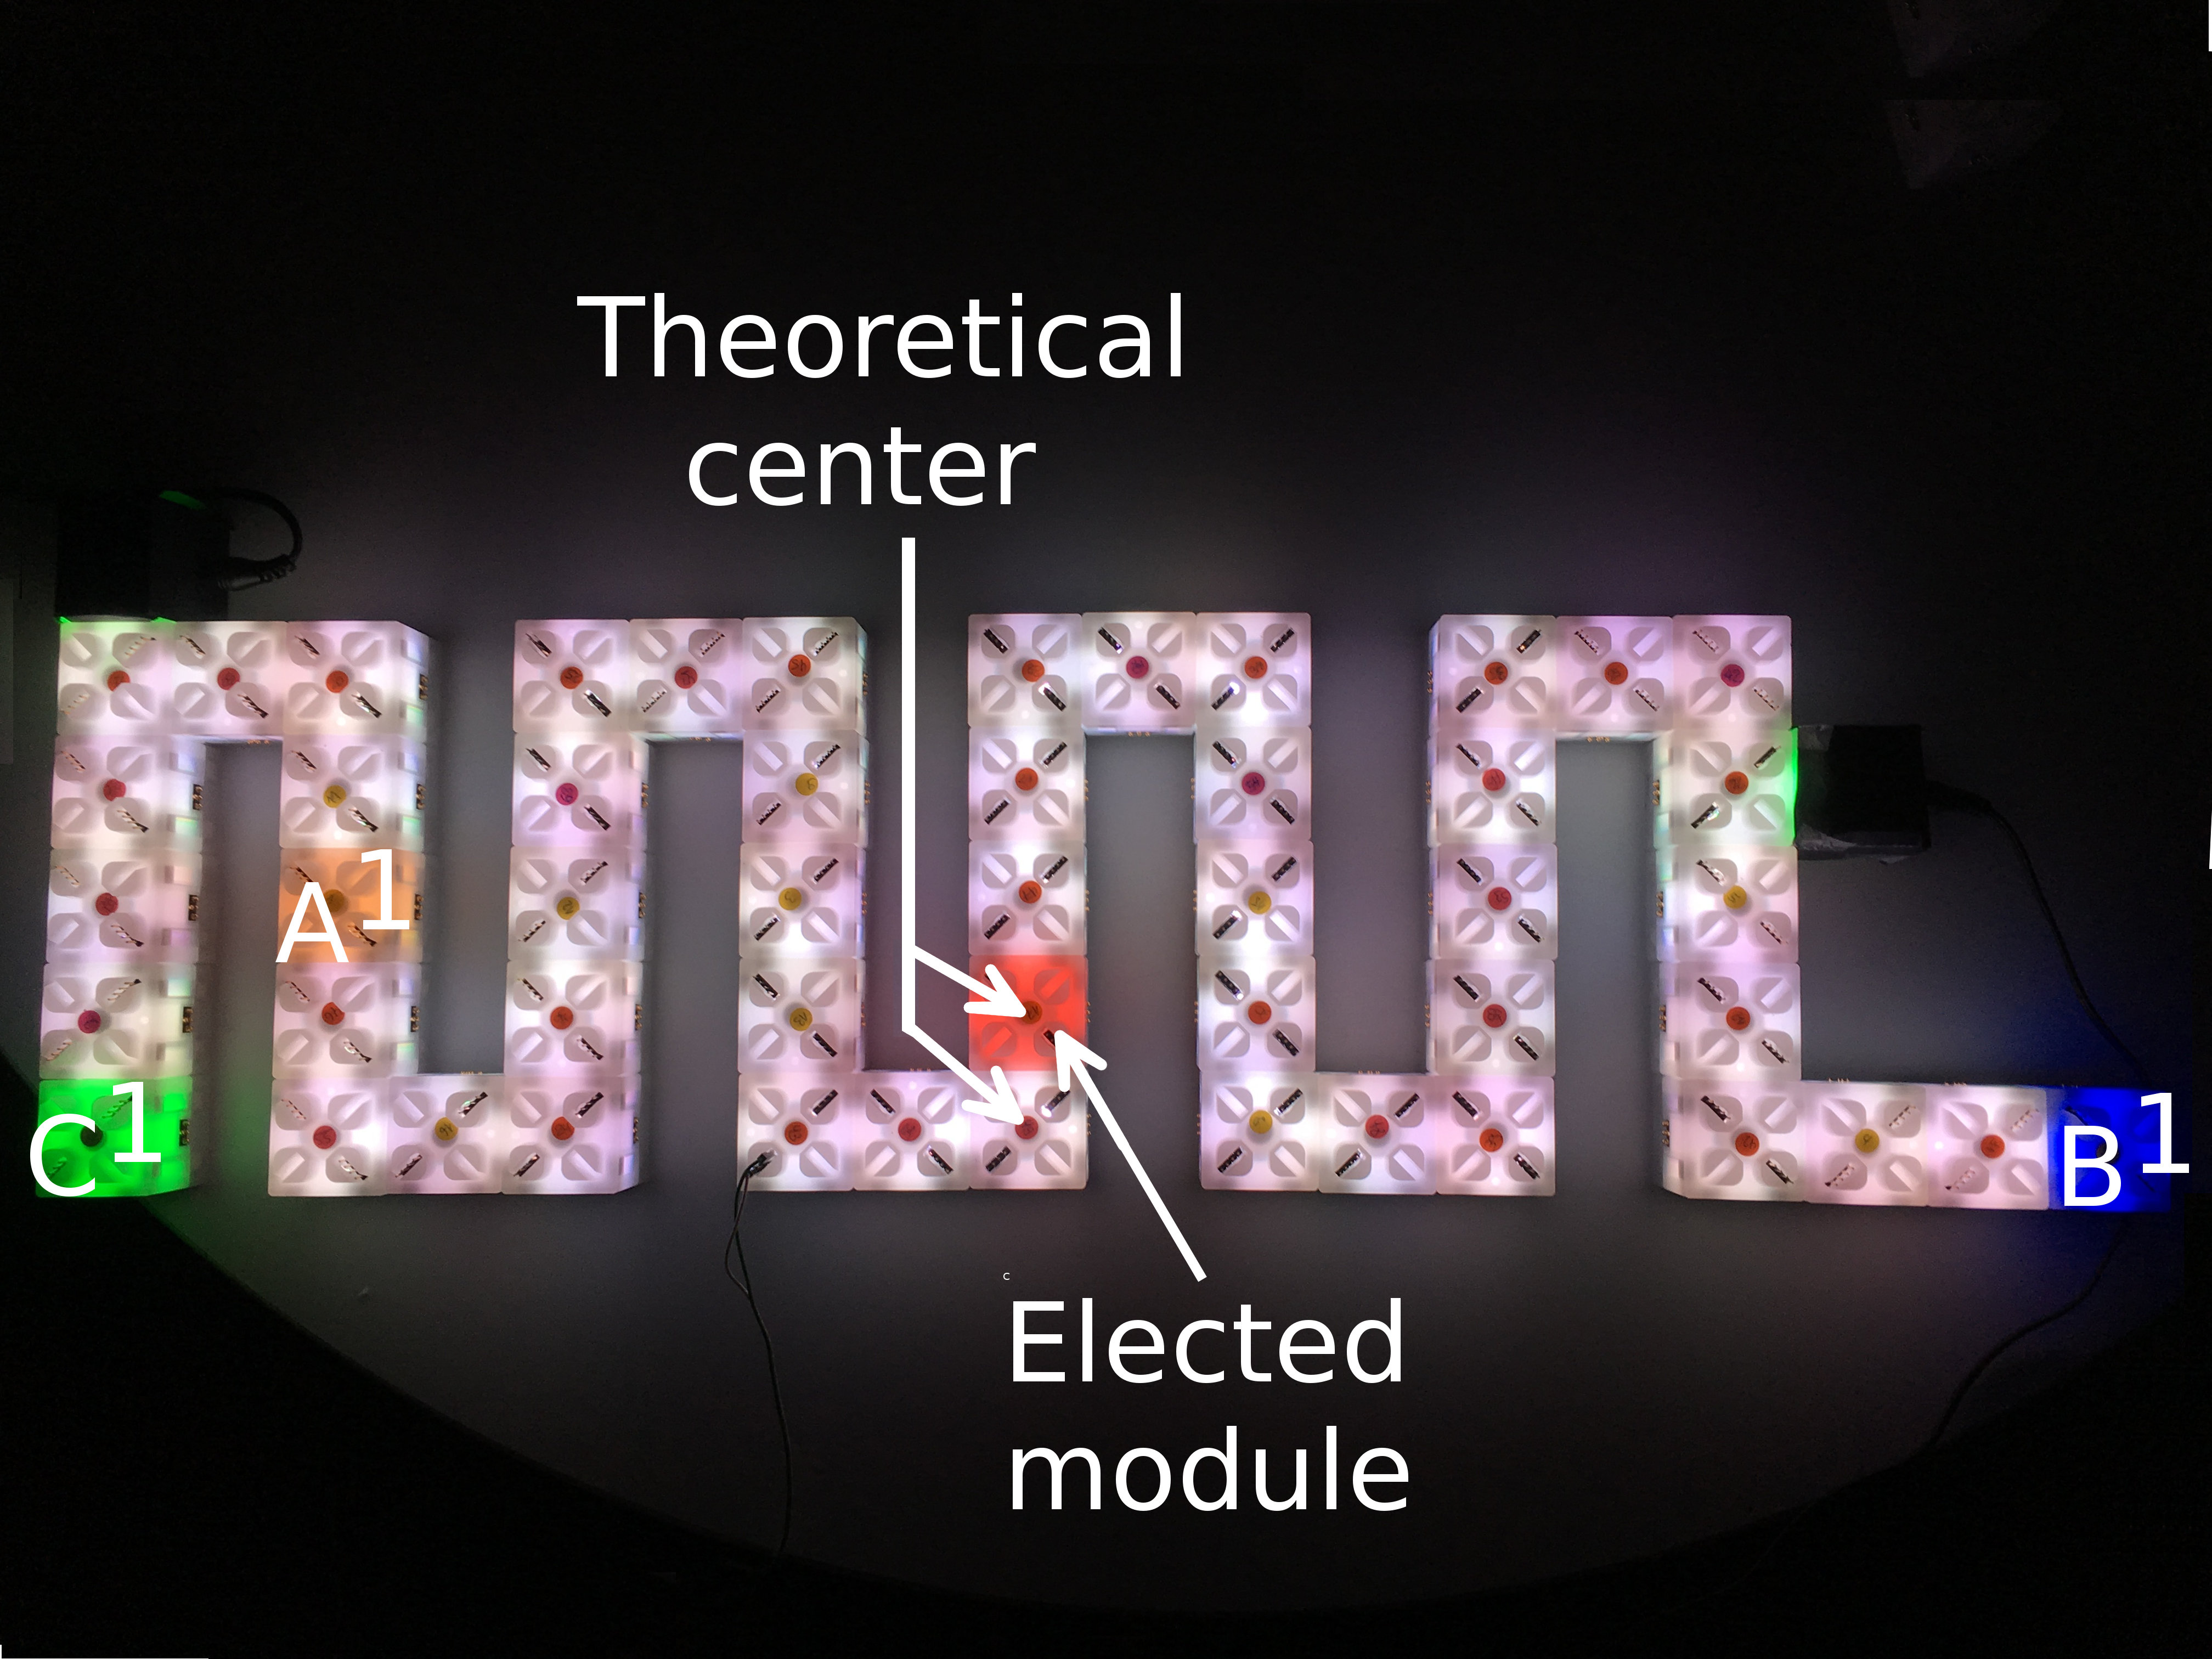
\includegraphics[width=\mySubfigureWidth,height=\mySubfigureHeight]{images/centrality/abc-centerv1-hardware/line-50-label.png} & 	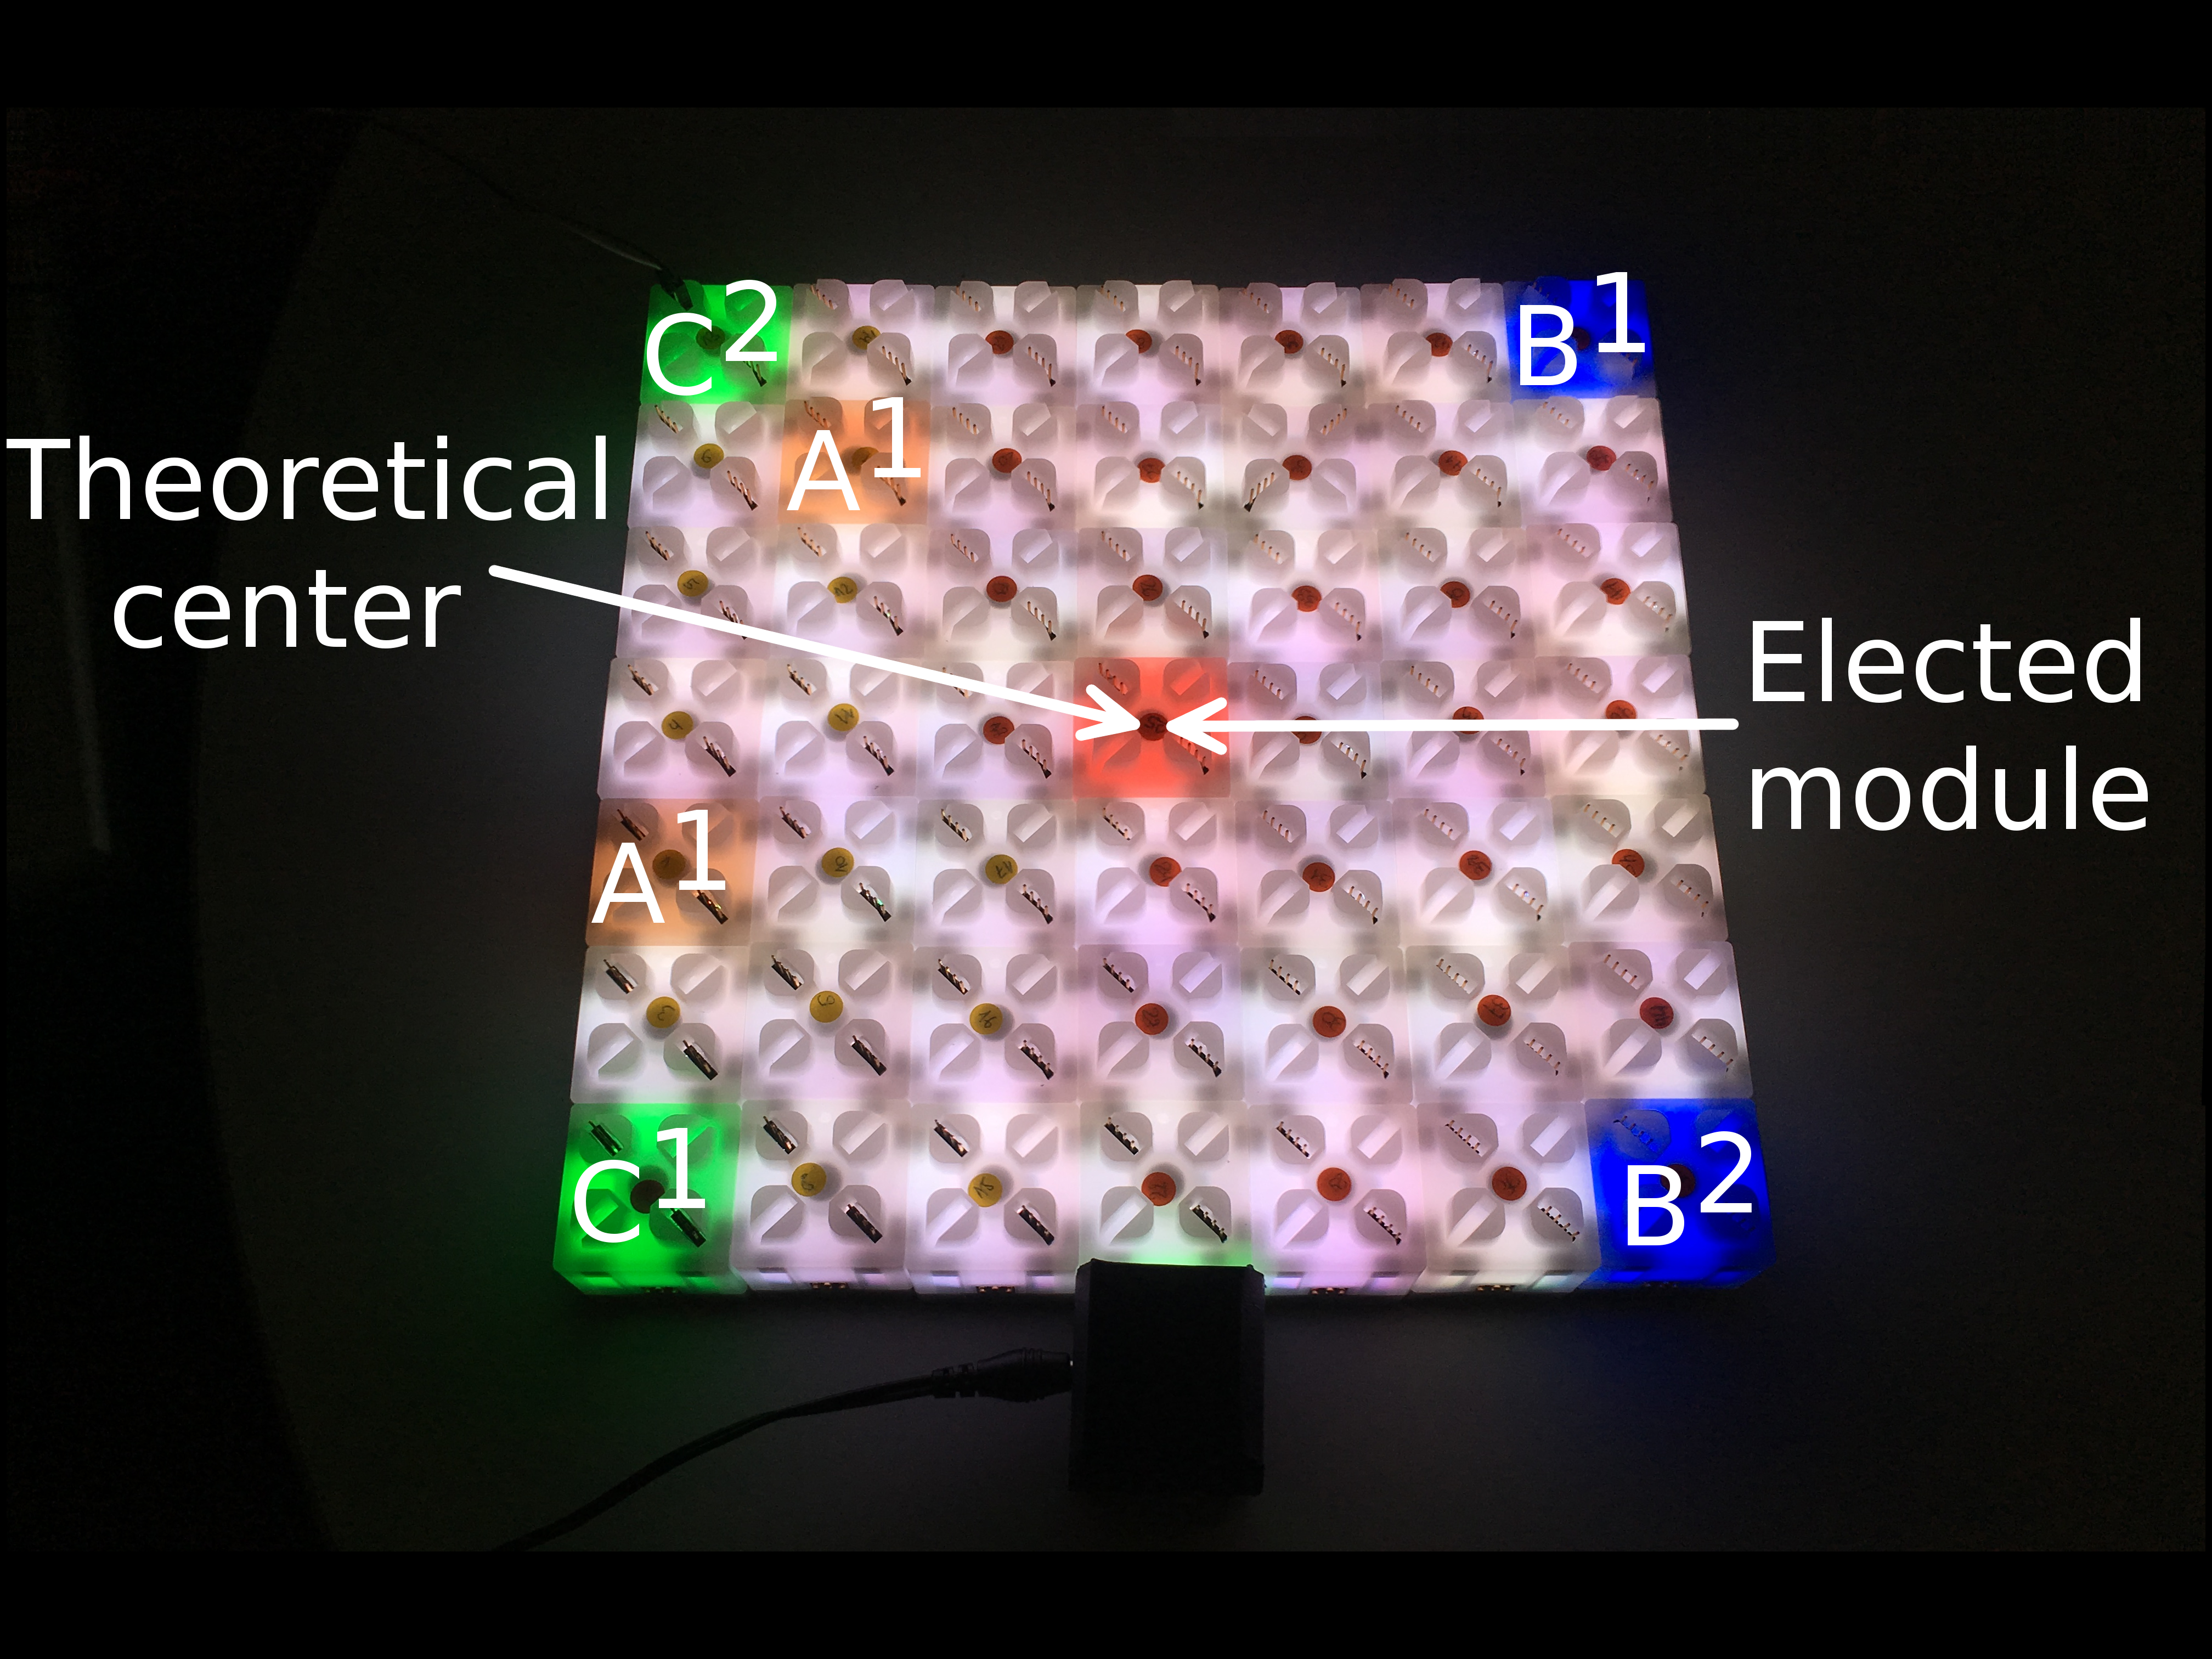
\includegraphics[width=\mySubfigureWidth,height=\mySubfigureHeight]{images/centrality/abc-centerv1-hardware/square-label-cropped-scalled.png}\\
			a) Line (50 modules). & b) Square (49 modules).\\
			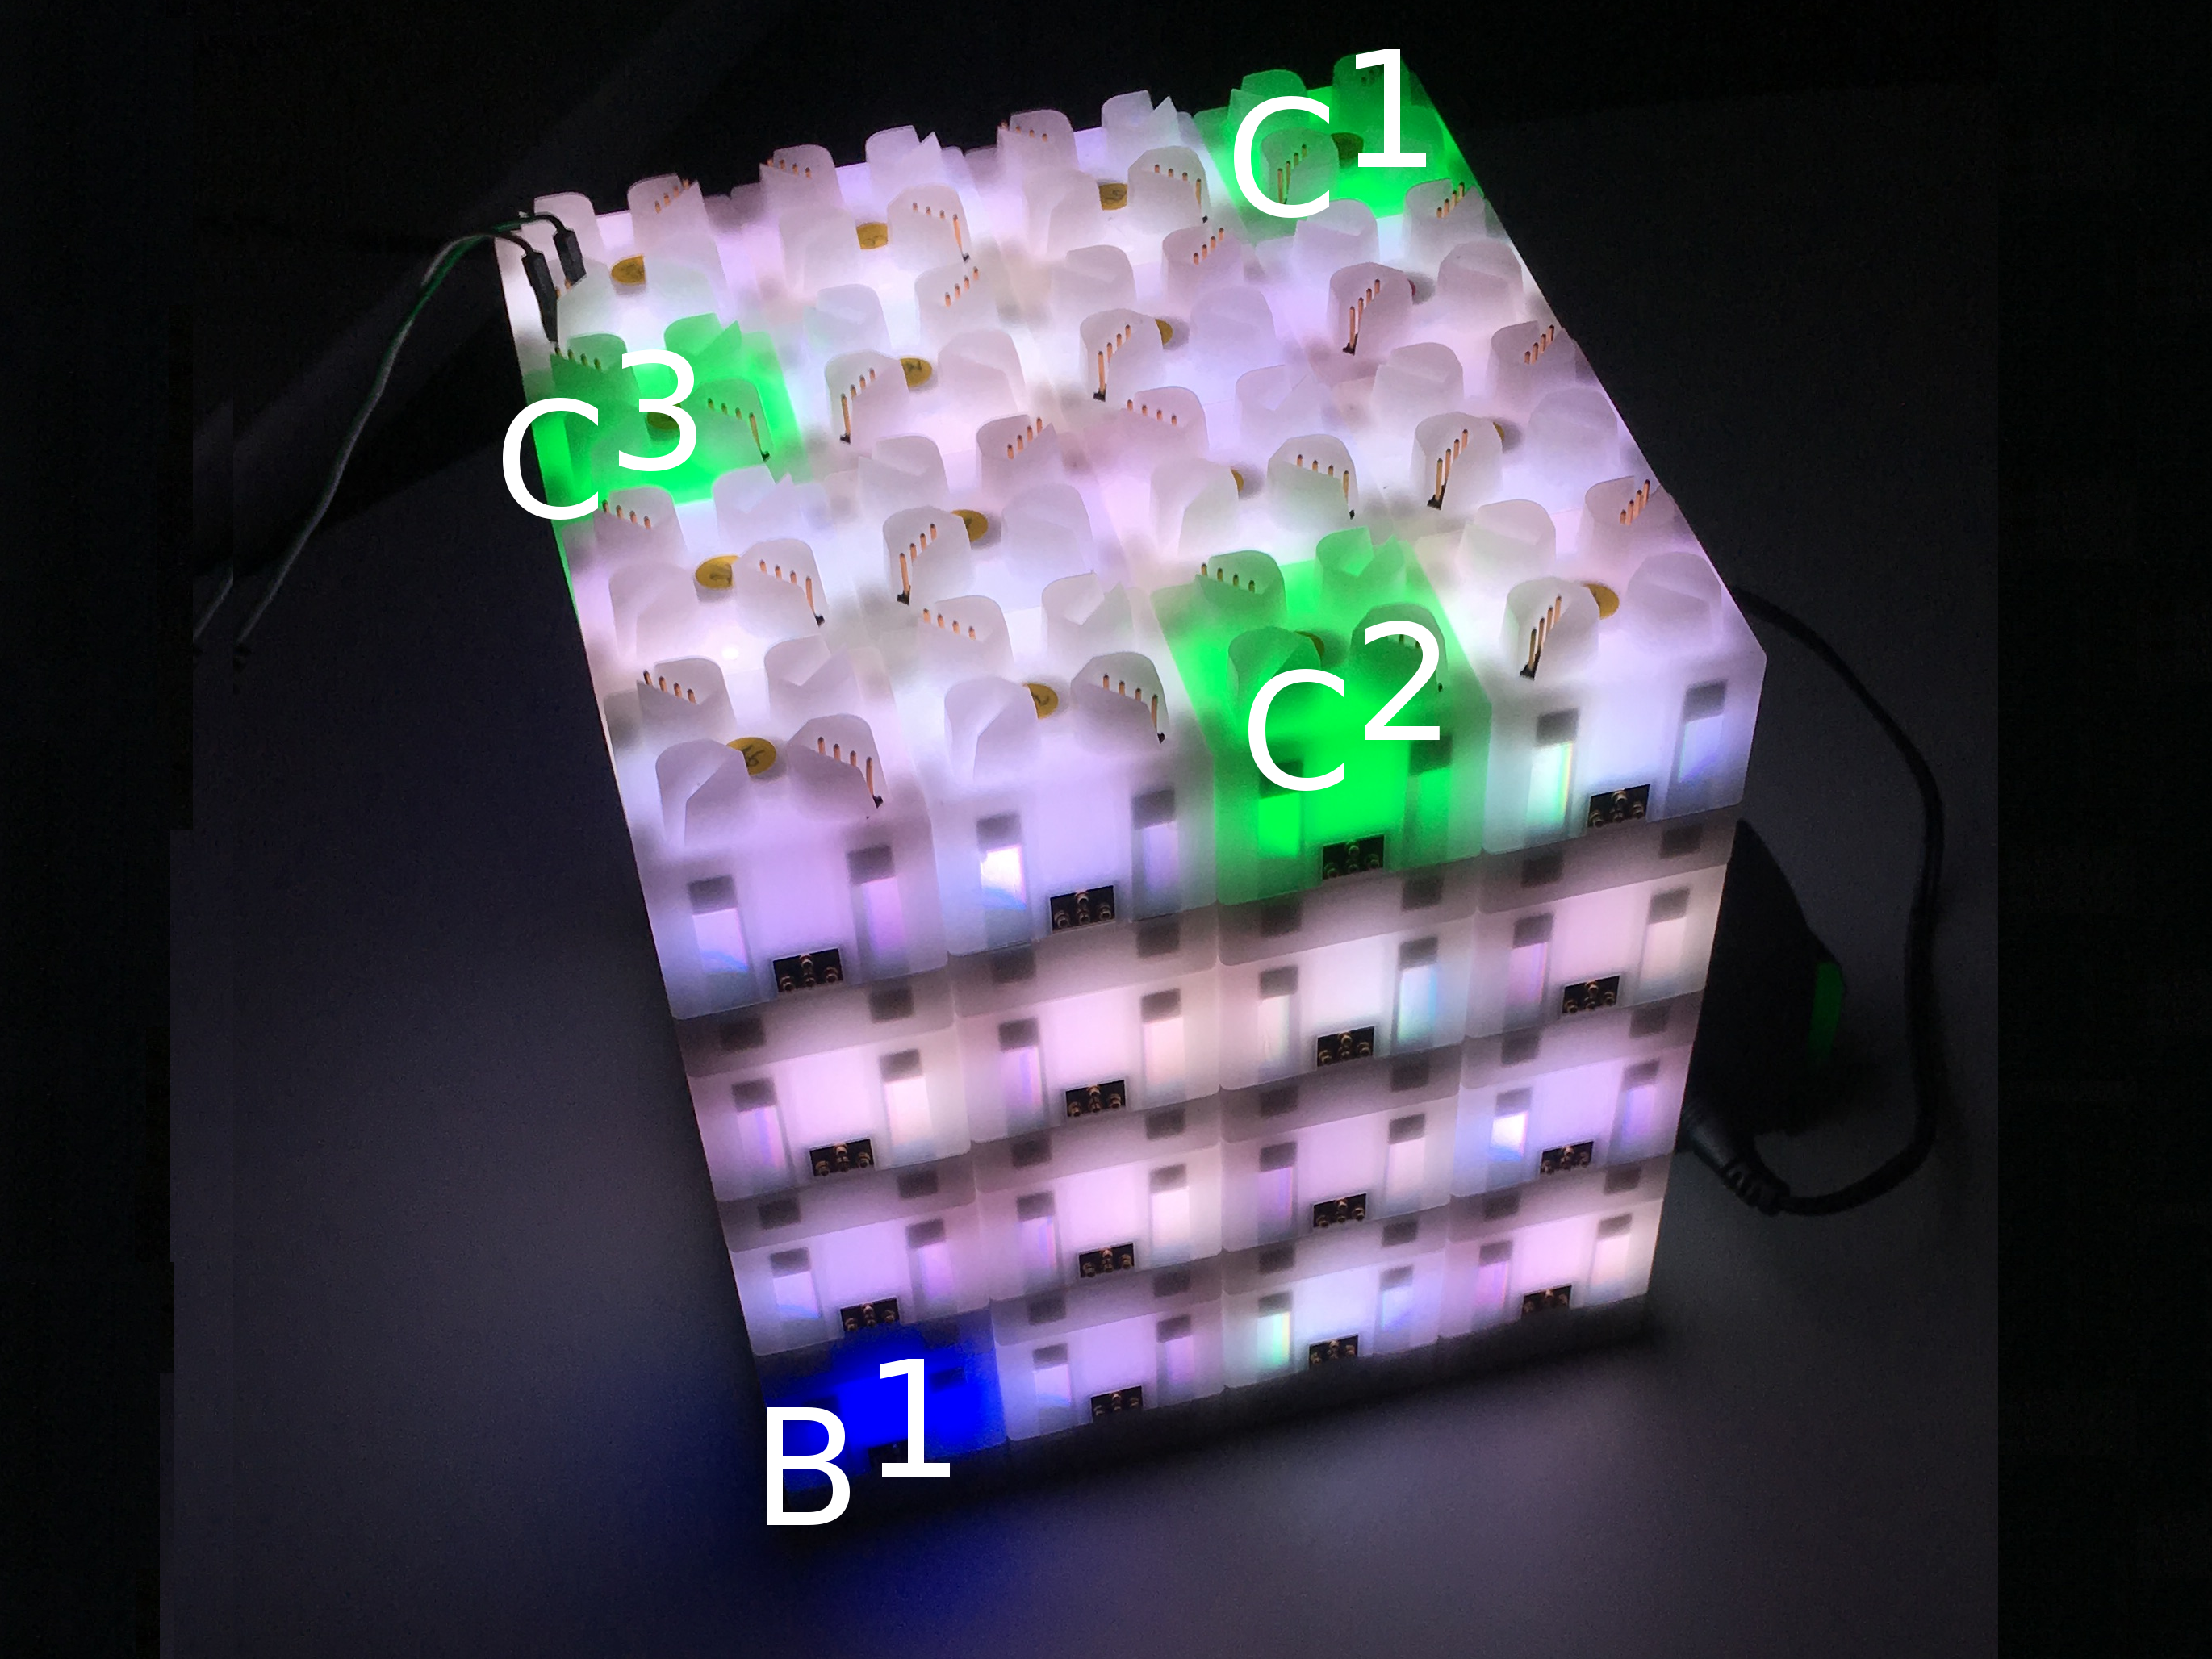
\includegraphics[width=\mySubfigureWidth,height=\mySubfigureHeight]{images/centrality/abc-centerv1-hardware/cube-label-rectangle-2.png} &
			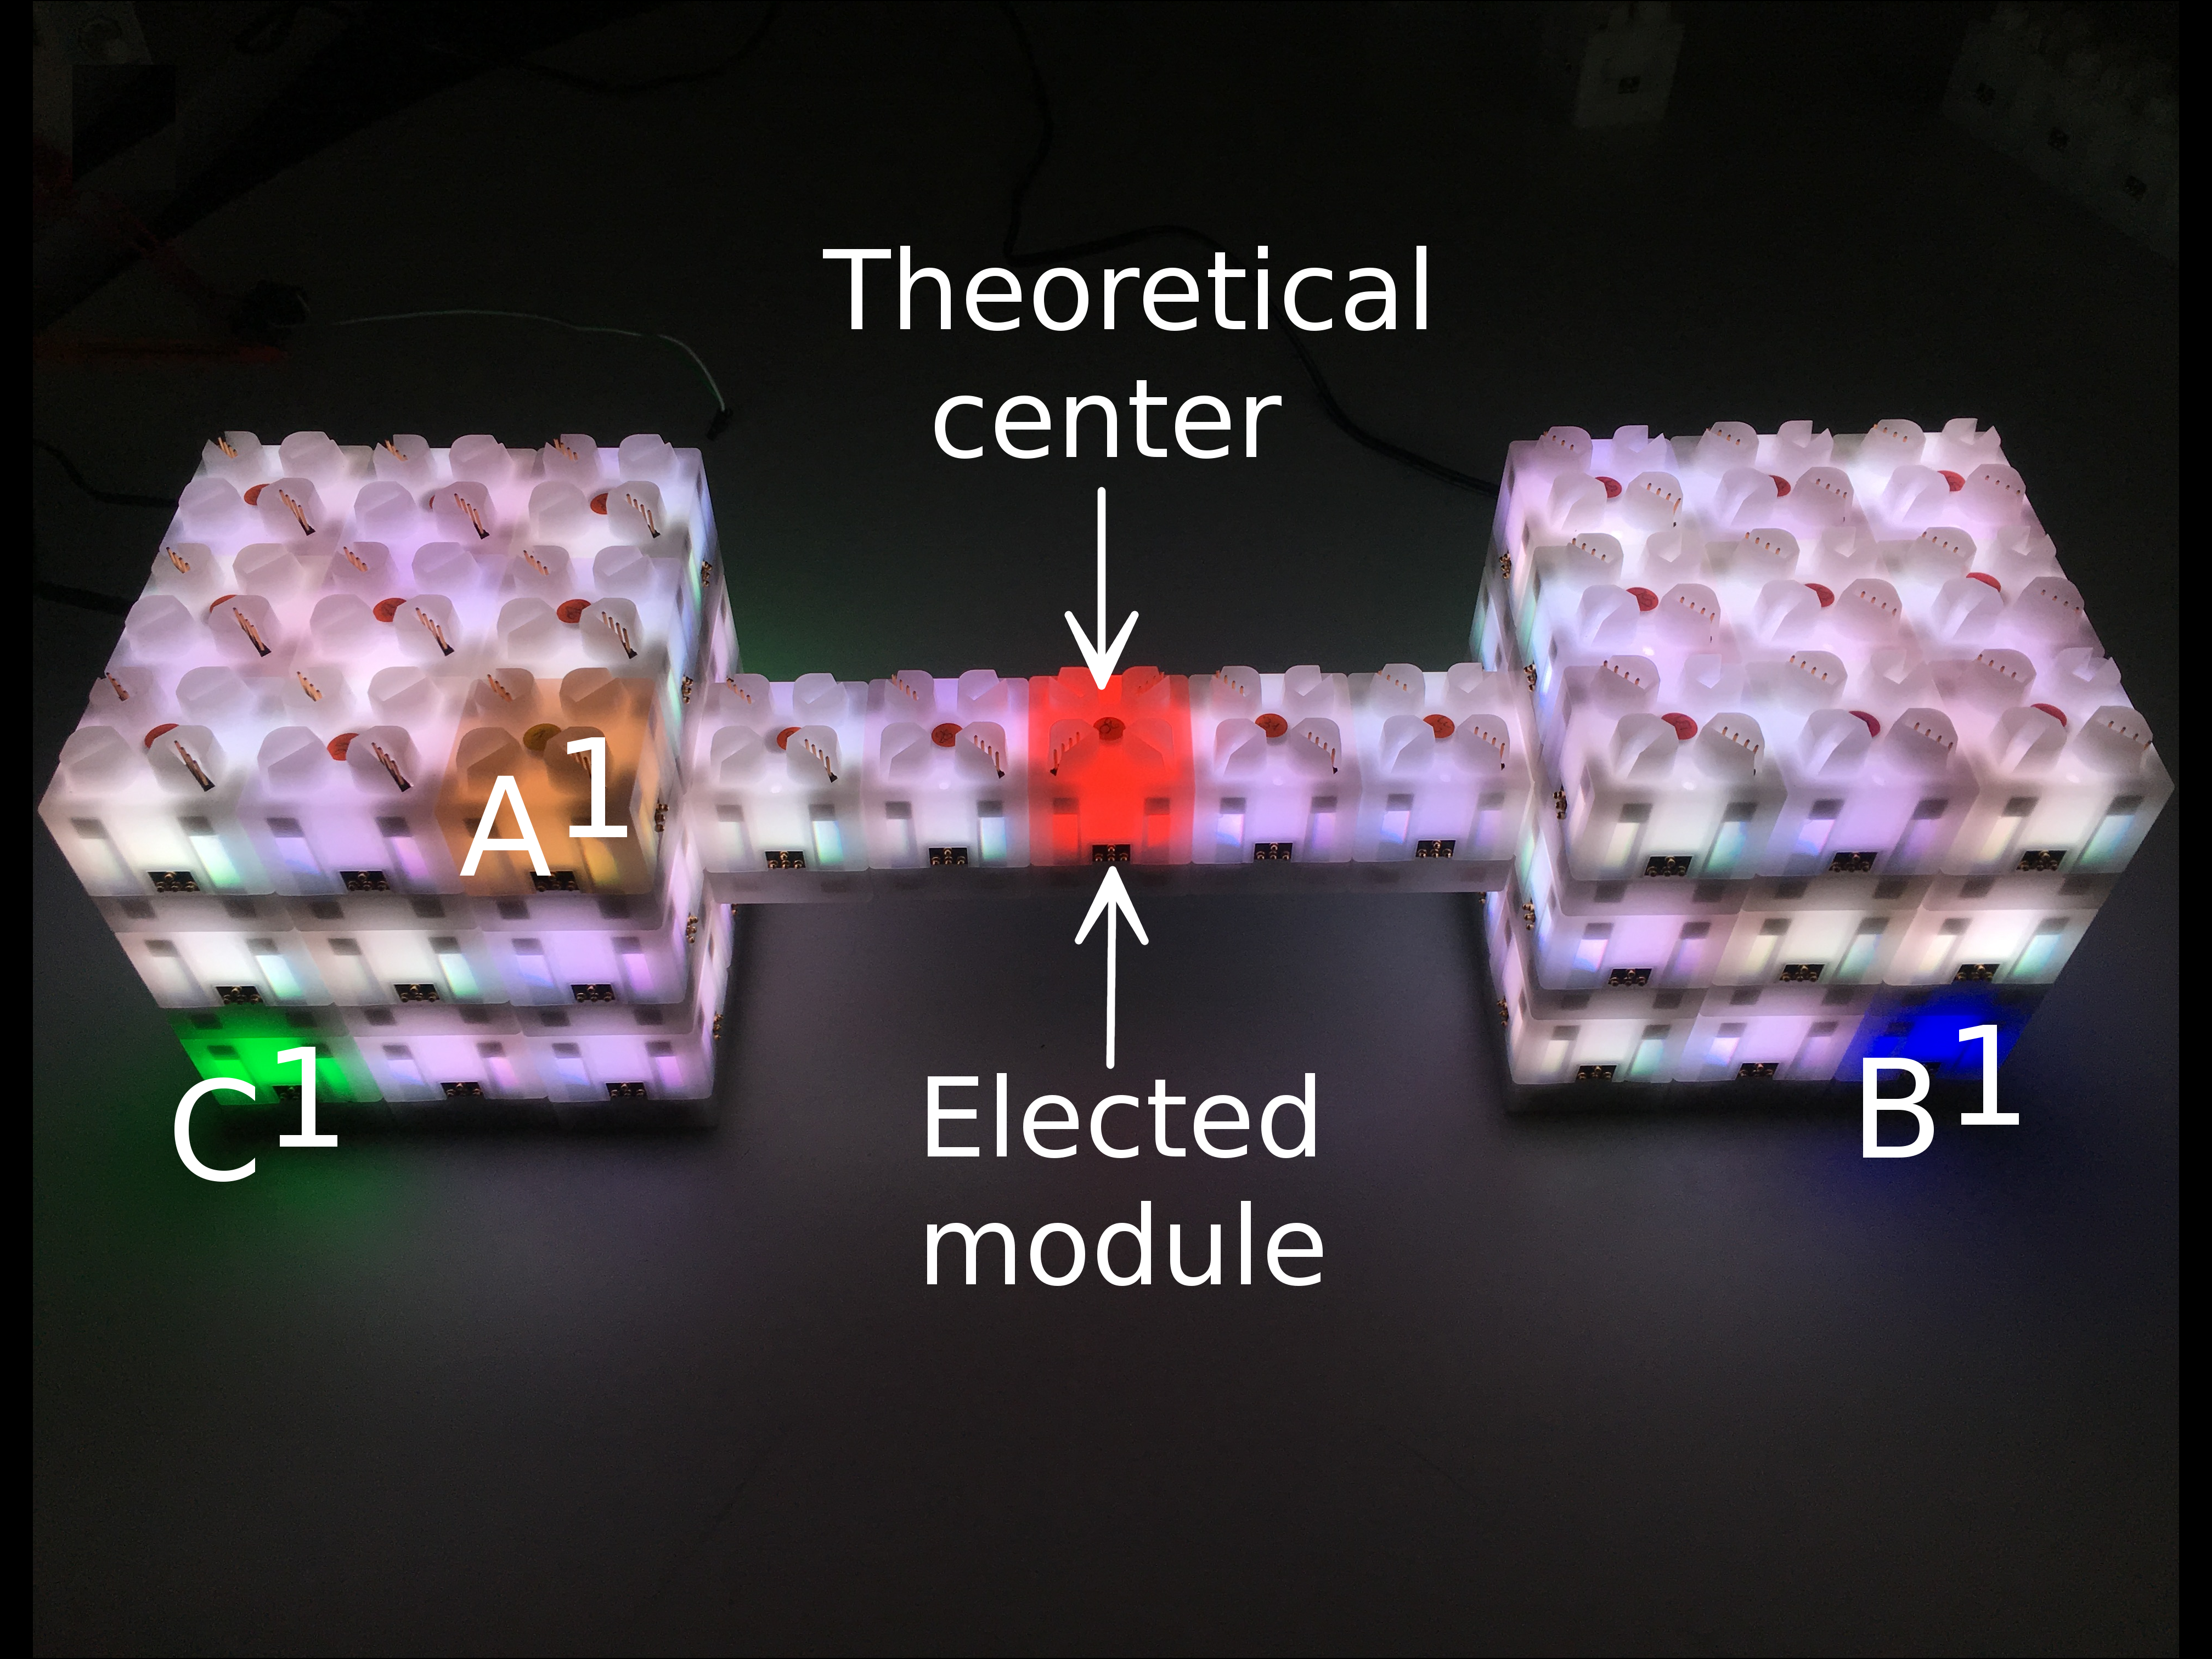
\includegraphics[width=\mySubfigureWidth,height=\mySubfigureHeight]{images/centrality/abc-centerv1-hardware/dumbbell-label-scalled.png} \\
			c) Cube (64 modules). & d) Dumbbell (59 modules).\\
		\end{tabular}
		\caption{ABC-CenterV1 executions on different hardware Blinky Blocks configurations.\label{fig:centrality:abc-center-hardware}}
	\end{figure}
}

Table~\ref{table:centrality:results-abc-center-hardware} gives the execution times of ABC-CenterV1 in these configurations on different scales formed from 5 to 64 modules. The execution time depends on the diameter of the system and on the number of steps of our algorithm. We observe that the number of steps does not only depend on the geometrical dimension of the system shape (e.g., a 3D cube needs 3 steps, while a 3D dumbbell requires only 1 step like the line).

{
	\newcommand{\lenOneOne}{0.07\linewidth}
	\newcommand{\lenTwoTwo}{0.12\linewidth}
	\newcommand{\lenThreeThree}{0.15\linewidth}
	\begin{table}[!h]
		\centering			
		\small
		\begin{tabular}{|C{\lenThreeThree}|C{\lenThreeThree}|C{\lenThreeThree}|C{\lenOneOne}|C{\lenTwoTwo}|C{\lenTwoTwo}|}
			\hline
			& & & \multicolumn{3}{c|}{ABC-CenterV1} \\
			\cline{4-6}
			& & & & \multicolumn{2}{c|}{Average execution}\\
			Shape & Size (module) & Diameter (hop) & \# steps & \multicolumn{2}{c|}{time $\pm$ standard}\\
			& & & & \multicolumn{2}{c|}{deviation (ms)}\\
			\cline{5-6}
			&  & &  & Hardware & Simulator \\
			\hline
			\multirow{3}{*}{Line}  & 5 & 4 & \multirow{3}{*}{1} & $234 \pm 1$ & $244 \pm 3$ \\
			\cline{2-3}
			\cline{5-6}
			& 10 & 9 & & $545 \pm 5$ & $544 \pm 5$ \\
			\cline{2-3}
			\cline{5-6}
			& 50 &49 & & $2873 \pm 23$ & $2885 \pm 17$  \\
			\hline
			\multirow{3}{*}{Square} & 9 & 4 & \multirow{3}{*}{2} & $598 \pm 45$ & $588 \pm 14$\\
			\cline{2-3}
			\cline{5-6}
			& 25 & 8 & & $1117 \pm 30$ & $1119 \pm 27$ \\
			\cline{2-3}
			\cline{5-6}
			& 49 & 12 & & $1684 \pm 48$ & $1686 \pm 44$ \\
			\hline
			\multirow{2}{*}{Cube} & 27 & 6 &\multirow{2}{*}{3}  &$ 1229 \pm 56$ & $ 1214 \pm 31$\\
			\cline{2-3}
			\cline{5-6}
			& 64 & 9 & & $1927 \pm 51$ & $1941 \pm 33$\\
			\hline
			Dumbbell & 59 & 15 & 1 & $1262 \pm 56$ & $1252 \pm 57$\\
			\hline
		\end{tabular}
		\caption{Average execution time of ABC-CenterV1 on hardware Blinky Blocks and in simulations. Statistics on the execution time were computed over 25 runs for every configuration. Simulation timing results were computed several times, each time on 25 independent runs, and we kept the values that matched best the hardware execution time.\label{table:centrality:results-abc-center-hardware}}
	\end{table}
}



% initialization: 24.97 - 2.51 = 2.46s
% re-election: 11.675 - 9.67 = 2.05
% Detecting new neighbors / departure takes up to 500 milliseconds.

Figure~\ref{fig:centrality:abc-center-network-dyanmics} illustrates ABC-CenterV1 tolerance to network dynamics. The system initially forms a 7x7 square. Modules take about 2.5 seconds to boot up, initialize themselves, discover their neighborhood and elect their center. An extra arm of 11 Blinky Blocks is then connected to the square-shaped ensemble which detects the network change and elects its new center in approximately 2 seconds. Note that ABC-CenterV1 is locally launched on a module at the earliest: 1 second after the module complete initialization using a software timeout, 1 second after a neighbor change detection or upon reception of an ABC-CenterV1 message. New neighbors are detected in a few hundred milliseconds.

{
	\newcommand{\subFigureWidth}{0.425\linewidth}
	\begin{figure}[h!]
		\centering			
		\small
		\begin{tabular}{c c}
			\includegraphics[width=\subFigureWidth]{images/centrality/abc-centerv1-dynamics/0}  &
			\includegraphics[width=\subFigureWidth]{images/centrality/abc-centerv1-dynamics/1}\\
			a) System of 49 nodes starts up. & b) ABC-Center terminates.\\
			\includegraphics[width=\subFigureWidth]{images/centrality/abc-centerv1-dynamics/2} &
			\includegraphics[width=\subFigureWidth]{images/centrality/abc-centerv1-dynamics/3}\\
			c) Adding 11 nodes. & d) ABC-Center terminates.\\
		\end{tabular}	
		\caption{ABC-CenterV1 execution in a dynamic network.\label{fig:centrality:abc-center-network-dyanmics}}
	\end{figure}
}

\subsection{Simulation Model and Fidelity}

This section shows the simulation model we have implemented in VisibleSim to simulate the behavior of the Blinky Blocks. Our model takes into account the processing time, the queuing time and the communication time (see Table~\ref{table:centrality:centrality-simulation-model}).

{
	\newcommand{\lenOneTwo}{0.12\linewidth}
	\newcommand{\lenTwoTwo}{0.14\linewidth}
	\newcommand{\lenThreeTwo}{0.21\linewidth}
	\newcommand{\lenFourTwo}{0.30\linewidth}
	\newcommand{\lenFourThree}{0.40\linewidth}
	\begin{center}		
		\small
		\begin{table}[h!]
			\centering
			\begin{tabular}{|C{\lenTwoTwo}|C{\lenFourTwo}|C{\lenFourThree}|}
				\hline
				\multicolumn{2}{|c|}{Parameters} & Value\\
				\hline				
				\multirow{3}{*}{\begin{minipage}{\linewidth}\centering Transfer rate $(kbit/s)$\end{minipage}} & $ |N_{v_i}^1| \leq 2 $ & $\mathcal{N}(28.331,1.112)$ \\
				\cline{2-3}
				& $ 2 < |N_{v_i}^1| \leq 4 $ & $\mathcal{N}(26.667,2.471)$ \\
				\cline{2-3}
				& $ 4 < |N_{v_i}^1| \leq 6 $ & $\mathcal{N}(25.846,2.471)$ \\
				\hline
				\multicolumn{2}{|c|}{Processing time $(s)$} & $\mathcal{U}(25\times10^{-6},125\times10^{-6})$ \\
				\hline
			\end{tabular}
			\caption{Communication model. $\mathcal{N}(\mu,\sigma)$ refers to the normal probabilistic law with $\mu$ being the mean and $\sigma$ the standard deviation. $\mathcal{U}(l,u)$ refers to the uniform probabilistic law with the minimum value $l$ and the maximum value $u$.}\label{table:centrality:centrality-simulation-model}
		\end{table}
	\end{center}
}

The processing time represents the time necessary to handle an incoming message. We used the micro-controller clock running at 32~MHz (nano-second scale resolution) to measure the processing time of different message handlers and arbitrarily chose to simulate the processing time using a uniform distribution with the range of the measured time.

In our work on time synchronization presented in Chapter~\ref{chapter:time-synchronization}, we estimate the transfer rate between neighboring modules using round-trip time measurements (see Section~\ref{section:time-sync:model}). The transfer rate corresponds to the communication rate from the data-link layer to the data-link layer of neighboring nodes. We observed that the transfer rate depends on the number of simultaneous communications. In this section model, the communication rate depends on the size of the neighborhood of a node.

The reader may have noted that the simulation model presented here differs from the model we use in Chapter~\ref{chapter:time-synchronization}. There are several reasons for that. Firstly, we use here some newly fabricated Blinky Blocks hardware with some different hardware components (e.g., the network connectors). Secondly, their firmware is slightly modified as well. In particular, we have reduced the time a module needs to find a free frame using dynamic frame allocation instead of a static array of frames with a free-frame search cost of $O(\text{\# static frames})$. This reduces the message processing time as modules require less time to send messages in response to incoming ones. Last but not least, we use here a less fine-grained simulation model for the sake of time efficiency. For instance, we do not check every single byte of a message for special bytes to escape; instead, we only increase the average and the standard deviation of the communication rate to mimic that phenomenon. We slightly adapt the transfer rate in order to obtain simulation times that match the ABC-CenterV1 execution time on new Blinky Blocks hardware prototypes.

Table~\ref{table:centrality:results-abc-center-hardware} shows that the simulated execution times on VisibleSim closely match the execution time obtained experimentally on hardware Blinky Blocks, for small and larger configurations, and for sparse (e.g., lines), less-sparse (e.g., squares), compact (e.g., cubes) and mixed-density configurations with compact components linked by a critical path (e.g., the dumbbell). Thus, VisibleSim can be used to accurately benchmark the performance of our algorithms on much bigger configurations.

\subsection{Large-scale Evaluation and Comparison to Existing Algorithms}

We use VisibleSim to evaluate the performance of our algorithms and to compare them with existing ones in terms accuracy, execution time, number of messages and memory usage on random large-scale Blinky Block systems. Random systems were generated by connecting the modules one by one to the system at random, starting from a single node. This guarantees the connectivity of the network and tends to generate compact systems with a reasonable diameter. Modules have a unique identifier in  $\{1..n\}$. Unless explicitly mentioned, every single point on the result plots represents 50 independent executions.

\subsubsection{Compared Algorithms and Parameters}
\label{section:centrality:compared-algorithms}

We compare our algorithms to several approaches that we potentially ported to fit our system models.

% Reference: https://gist.github.com/badboy/6267743
%hash function: 
% Knuth's multiplicative hash function \cite{knuth1998art}
% Fowler–Noll–Vo 1 (FNV-1) hash function~\cite{fowler1991fnv}
% FNV1: hashes are designed to be fast while maintaining a low collision rate. 
%Murmur3 32bit hash function~\cite{appleby2011Murmur3} which was designed to be fast while maintaining a low collision rate

% Affine function $h(x) = (a*x + b) mod (2^{32}-1)$ where $a$ and $b$ are large prime numbers / small odd numbers. Including the identitiy function h(x) = x.
% Murmur3 32-bit hash function~\cite{appleby2008Murmur3}
% random numbers

% probabilistic counter:
% see talk (slide 49/51): https://www.cs.princeton.edu/~rs/talks/AC11-Cardinality.pdf
% HyperLogLog size : //https://blog.demofox.org/2015/03/09/hyperloglog-estimate-unique-value-counts-like-the-pros/

\newcommand{\myParagraph}[1]{\textit{#1: }}

\myParagraph{Our work} We consider ABC-CenterV1, ABC-CenterV2, $k$-BFS SumSweep, PC2LE and the algorithm we proposed in~\cite{npgb16b:ip}. We use the following parameters:
	\begin{itemize}
		\item In the $k$-BFS SumSweep framework, we arbitrarily choose $k = 10$. 
		
		\item In our implementation of PC2LE, we use the HyperLogLog~\cite{flajolet2007hyperloglog} probabilistic counter using 16 registers of 5 bits each for a total of 80 bytes with the 32-bit Knuth multiplicative hash function~\cite{knuth1998art}. Actually, we experimentally compared several combinations of counters (the Flajolet-Martin~\cite{flajolet1985probabilistic} and HyperLogLog~\cite{flajolet2007hyperloglog} counters) and hash functions (affine functions, Knuth's multiplicative hash functions~\cite{knuth1998art}, the MurMur3~\cite{appleby2011Murmur3} hash function and the FNV hash function~\cite{fowler1991fnv}). Probabilistic counting involves a trade-off between the memory space used by the counter and its accuracy. In our tests, we limit the size of the different counters so that any PC2LE message fits into a single Blinky Blocks frame, i.e., a counter can occupy 10 bytes at most. We choose the HyperLogLog along with the Knuth multiplicative hash function as it leads to more accurate results. For the reader's information, the Flajolet-Martin counter based on five 16-bit affine functions $h(x) = ax+b$, where $a$ and $b$ are small odd numbers, also performs very well.
		
		\item In~\cite{npgb16b:ip}, we proposed the E2ACE (Efficient and Effective Approximate-Centroid Election) algorithm which approximately corresponds to the centroid version of PC2LE based on the Flajolet-Martin probabilistic counter combined with the identity hash function. To compare the accuracy of the current version of PC2LE with our early work, we also consider the PC2LE-FM-1 (Flajolet-Martin with the identity hash function) approach.
	\end{itemize}

\myParagraph{MIN-ID} we consider the minimum-id leader election algorithm in Section 4.5 of~\cite{raynal2013distributed}, extended with our controlled-broadcast optimization (see Section~\ref{section:centrality-controlled-broadcast}). As module identifiers are randomly attributed in the network, this corresponds to the election of a random node.

\myParagraph{BARYCENTER} We consider the exhaustive BARYCENTER algorithm presented in~\cite{mamei2005self}. It computes all-pair shortest paths using $n$ simultaneous asynchronous \gls{bfses} without acknowledgment. BARYCENTER was proposed as an application of the TOTA tuple-space-based middleware. We use our own implementation of this approach. In our implementation, modules wait for 500 milliseconds after the reception of the last distance update triggered by a \gls{bfs} message to check for convergence. Note that BARYCENTER does not have a global termination criterion and some nodes can temporarily recognize themselves as centroid. 

%%dissler2016distributed
\myParagraph{$k$-BFS-RAND} We consider our own distributed implementation of the sequential approach~\cite{eppstein2001fast} to approximate the node centrality using $k$ \gls{bfses} from random nodes. We refer to it as the $k$-BFS-RAND approach. To be fair in comparison with the $k$-BFS SumSweep framework, we also fix $k = 10$. In our implementation, every node generates a random number and the $k$ nodes of minimum generated number perform a \gls{bfs} (ties are broken arbitrarily). Every node estimates its partial farness/eccentricity values using the distance to the $k$ random nodes. In the $k$-BFS-RAND-SEQ, the \gls{bfses} are performed sequentially. The node of minimum generated number is elected as initiator using a variant of the \cheungIeCb{} algorithm. In $k$-BFS-RAND-PAR, the $k$ \gls{bfses} are performed in parallel. All nodes initiate a \gls{bfs}  using a variant of the \cheungCb{} algorithm modified with a mechanism to ensure that only the \gls{bfses} initiated by the $k$ nodes of minimum generated number terminate (i.e., 10 simultaneous elections). Node identifiers are used to break the ties. Note that $k$-BFS-RAND-PAR is prone to network congestion because our current version of the controlled-broadcast optimization does not enable to run multiple parallel elections. Once the $k$ \gls{bfses} have terminated, the node of minimum centrality value is elected using an STC followed by an STB on the tree rooted at the $k^{th}$ node.

\myParagraph{TBCE} We also consider the Tree-Based Center Election (TBCE) algorithm, our own implementation of the election of the node of maximum tree-based centrality~\cite{kim2013leader}. We choose this algorithm as it is both time- and memory-efficient.

\myParagraph{PC2LE-MC2} The algorithm proposed in~\cite{garin2012distributed} to estimate node eccentricity is not directly applicable because it targets synchronous distributed systems, because it requires providing an upper bound of the graph diameter and because it does not elect a node but only estimates every node eccentricity value. Thus, to evaluate the performance of the approach proposed in~\cite{garin2012distributed} in our target system, we use the PC2LE along with the probabilistic counter~\cite{varagnolo2010distributed} applied in~\cite{garin2012distributed}. We call this approach PC2LE-MC2 (Maximum-Consensus Counter).

\subsubsection{Effectiveness Evaluation}

In order to exhibit the accuracy of an algorithm, we use the relative center accuracy and the relative centroid accuracy (see Equations~\eqref{eq:relative-error-far} and~\eqref{eq:relative-error-ecc}). We have computed the exact center/centroid and node eccentricity/farness using our tool\footnote{GraphAnalyzer. Tool available online at: \GAURL{}} for external graph analysis.
\vspace{-1em}
\begin{align}
\equationTextSize
\label{eq:relative-error-far}
\parbox{15em}{\centering relative\ \ centroid accuracy}
= 1 - \left|\frac{far(centroid)- far(elected\ node)}{far(centroid)}\right|
\end{align}
\vspace{-1em}
\begin{align}
\equationTextSize
\label{eq:relative-error-ecc}
\parbox{15em}{\centering relative\ \ center accuracy} 
= 1 - \left|\frac{ecc(center)- ecc(elected\ node)}{ecc(center)}\right|
\end{align}

Figure~\ref{fig:centrality:accuracy} shows the relative center and centroid accuracy of the different algorithms considered. 

\begin{figure}[!h]
	\centering
	\includegraphics[width=0.85\linewidth]{images/centrality/accuracy}
	\caption{Effectiveness of centrality-based leader election algorithms: relative eccentricity and centroid accuracy versus the number of modules in the system. For frameworks, the centroid (resp. center) version is considered for the centroid (resp. center) accuracy.}
	\label{fig:centrality:accuracy}
\end{figure}

We observe that ABC-Center, PC2LE and $k$-BFS SumSweep are more accurate than the other algorithms. In systems with 25,000 modules, our algorithms provide a relative centroid accuracy between 96\%-99\% and a relative center accuracy between 88\%-94\%.  Note that ABC-CenterV2 seems slightly more precise at large scale than the other two.

Furthermore, we observe that performing BFSes from external nodes using the SumSweep heuristic (10-BFS-SUMSWEEP) leads to more accurate results than performing the BFSes from a random sample of nodes (10-BFS-RAND).

Moreover, using the HyperLogLog counter (PC2LE) with the PC2LE framework leads to more accurate results than using the maximum consensus-based probabilistic counter~\cite{varagnolo2010distributed} used in~\cite{garin2012distributed} (PC2LE-MC2) and than using the Flajolet-Martin algorithm with a single bitstring, as done in our early work~\cite{npgb16b:ip} (PC2LE-FM-1).


\subsubsection{Efficiency Evaluation}

In this section, we study the time efficiency, the communication efficiency and the memory usage of the different algorithms.

\paragraph{Simulated Execution Time}

To measure the execution time, we consider that an algorithm terminates when the node to be elected considers itself elected.

Figure~\ref{fig:centrality:time} shows that the simulated average execution time of all the considered algorithms except BARYCENTER seems to increase linearly with the diameter of the system. The average execution time of BARYCENTER explodes in systems with more than 1,000 modules. We believe that this is due to network congestion.

\begin{figure}[!h]
	\centering
	\includegraphics[width=\gnuplotGraphWidth]{images/centrality/time}
	\caption{Simulated average execution duration ($\pm$ standard deviation) of centrality-based leader election algorithms versus the system diameter. For each point, at least 5 executions were performed.\label{fig:centrality:time}}
\end{figure}

ABC-CenterV1, ABC-CenterV2 and $k$-BFS SumSweep are longer to converge than the other algorithms considered, except for BARYCENTER. Nevertheless, as previously shown, these algorithms tend to have better center accuracy results than all the others. To give an idea of the convergence time, ABC-Center requires on average 3-4 steps to converge in our systems. Also note that ABC-CenterV2 is slightly faster than ABC-CenterV1.

MIN-ID, TBCE, PC2LE and $k$-BFS-RAND-PAR scale well in terms of execution time. For Blinky Blocks systems with a diameter of more than 65 hops and a size of approximately 25,000 modules, MIN-ID, TBCE and PC2LE  respectively elect a central module in less than 1, 2 and 4 seconds. PC2LE is slightly slower than TBCE and MIN-ID, but is definitely more precise, as shown in the previous section.

\paragraph{Number of Messages}

Figure~\ref{fig:centrality:messages} shows the total number of messages exchanged during the execution of the centrality algorithms considered according to the size of the system. Figure~\ref{fig:centrality:avg-messages} shows the average number of messages sent per module.
The number of messages used by an algorithm includes all the messages that it generates, even those sent after the final node has been elected. The number of messages sent also reflects the energy consumption of the modules.

\begin{figure}[!h]
	\centering
	\includegraphics[width=\gnuplotGraphWidth]{images/centrality/messages}
	\caption{Average total number of messages ($\pm$ standard deviation) of centrality-based leader election algorithms according to the size of the system.\label{fig:centrality:messages}}
\end{figure}

\begin{figure}[!h]
	\centering
	\includegraphics[width=\gnuplotGraphWidth]{images/centrality/avgMessages}
	\caption{Average number of messages sent per node ($\pm$ standard deviation) of centrality-based leader election algorithms according to the size of the system.\label{fig:centrality:avg-messages}}
\end{figure}

We observe that BARYCENTER uses a lot more messages than the other algorithms. PC2LE tends to use more messages at large scale than ABC-CenterV2 and the sequential $k$-BFS approaches. Moreover, the latter approaches use more messages than TBCE and MIN-ID. For large-scale systems with 25,000 Blinky Blocks, PC2LE uses about $20\times10^6$ messages while ABC-CenterV2, $10$-BFS-SumSweep, $10$-BFS-RAND-SEQ use $6\times10^6$ messages and TBCE uses only about $3\times10^6$ messages.

ABC-CenterV1 uses fewer messages than ABC-CenterV2. $10$-BFS-SumSweep and $10$-BFS-RAND-SEQ approximately use the same number of messages. Notice that 10-BFS-RAND-PAR generates more messages than $10$-BFS-RAND-SEQ.
 
\begin{figure}[!h]
	\centering
	\includegraphics[width=0.9\linewidth]{images/centrality/memory-queue}
	\caption{Above, the maximum memory usage (considering both the local algorithm variables and the message queue usage) according to the size of the system. Below, the maximum message queue per module (considering both the incoming and outgoing queues).\label{fig:centrality:memory-queue}}
\end{figure}

\paragraph{Memory Usage}

Figure~\ref{fig:centrality:memory-queue} shows the maximum memory usage of the different algorithms. The memory usage of an algorithm is composed of its memory footprint, both at the application level and in the different message queues. Note that in the Blinky Blocks firmware, whenever a module broadcasts a message to all its neighbors, a copy of the message is inserted in all its outgoing-message queues. Moreover, the Blinky Blocks store a message using 19 bytes of memory (17 bytes of data and 2 bytes for data related to message handling).

We recall that, in BARYCENTER, every node locally stores $O(n)$ information at the application level and PC2LE stores $O(c + \Delta)$, where $c$ is the cost of the probabilistic counter used. The other algorithms store $O(\Delta)$ information.

ABC-CenterV2, MIN-ID, PC2LE, $k$-BFS-SumSweep, $k$-BFS-RAND-SEQ and TBCE scale well in terms of memory usage. In systems with 25,000 nodes, they use less than 500 bytes of memory, among which 380 bytes\footnote{$20\times19 = 380$ bytes} are due to message queue occupancy. ABC-CenterV1 and $10$-BFS-RAND-PAR use up to 10 kbytes in systems with 25,000 modules because of the memory overhead due to message pileups. $10$-BFS-RAND-PAR perform \gls{bfses} in parallel, thus being faster but requiring much more memory. BARYCENTER uses 600 kbytes in systems with 5,000 modules.

\section{Discussion}
Electing a central node involves a trade-off between the cost that can be afforded in terms of resources (time, memory, computation, energy) and the desired level of accuracy. Thus the algorithm to be used in order to elect a central node depends on the application, i.e., the role that this central node will play, the stability of the network, the scarcest resource, etc. 

Exact approaches (e.g., BARYCENTER) are exhaustive and tend to overwhelm the network. They are definitely not suitable for large-scale systems since they are slow to converge, they generate a significant number of messages and may have a large memory footprint. It is paradoxical, since the importance of central nodes increases with the system size. In 5,000 node systems, BARYCENTER requires nearly 45 seconds to converge and uses more than 500 kbytes per node.

Electing a random node using MIN-ID leads to poor accuracy but scales well in terms of efficiency. TBCE provides a better accuracy while being only slightly slower and using a similar number of messages. In systems of 25,000 modules, TBCE runs on average in 2.3 seconds and has a relative centroid (resp. center) accuracy of 81\% (resp. 64\%).

We proposed PC2LE which is slightly slower than TBCE but is definitely more accurate. In systems of 25,000 modules, PC2LE runs in 3.3 seconds and provides a relative centroid accuracy of 96\% and a relative center accuracy of 88\%. However, this better accuracy comes at the price of a higher message cost.

We proposed ABC-CenterV2 and $k$-BFS-SumSweep which are the most accurate center approximation algorithms. They perform \gls{bfses} from specific nodes, which leads to more accurate results than computing \gls{bfses} from random nodes as in $k$-BFS-RAND. In 25,000 Blinky Blocks systems, ABC-CenterV2 elects, on average, a 99\% accurate centroid and a 94\% accurate center. ABC-CenterV2 and the $k$-BFS-SumSweep are, however, slow to converge as the \gls{bfses} are performed consecutively. In 25,000 module systems, they run in almost 13 seconds. These two algorithms use more messages than PC2LE and MIN-ID but less messages than PC2LE.

\gls{bfses} cannot be parallelized in ABC-CenterV2 and $k$-BFS-SumSweep, but if it was possible, naively performing \gls{bfses} in parallel would overwhelm the network and incur a large memory overhead. Indeed, $k$-BFS-RAND-PAR, which performs $k$ \gls{bfses} in parallel, uses at most 10 kbytes per node, while $k$-BFS-RAND-SEQ, in which the $k$ \gls{bfses} are computed consecutively, only uses 423 bytes.

ABC-CenterV2, $k$-BFS SumSweep, MIN-ID, TBCE and PC2LE all have a limited memory cost. They use between 400 and 480 bytes per node max.

\section{Conclusion}
\label{section:centrality:conclusion}

In this chapter, we proposed a collection of efficient and effective distributed algorithms to elect approximate-centroid and approximate-center nodes in asynchronous distributed systems. We evaluated our algorithm on the Blinky Blocks modular robotic system, using both hardware experiments and simulations. Results show that our algorithm scales well in terms of accuracy, execution time, number of messages and memory usage. To the best of our knowledge, our algorithms are the most precise existing distributed algorithms dedicated to the election of an approximate centroid or an approximate center in our target systems, with both a reasonable convergence time and a limited storage cost.

In the next chapter, we study time synchronization in \gls{lmrs}. We use the algorithms proposed in this chapter to elect a central node that synchronizes all the others. As shown in the Introduction section of this chapter, using a central module rather than a random one leads to more precision.